\documentclass[twoside]{book}

% Packages required by doxygen
\usepackage{fixltx2e}
\usepackage{calc}
\usepackage{doxygen}
\usepackage[export]{adjustbox} % also loads graphicx
\usepackage{graphicx}
\usepackage[utf8]{inputenc}
\usepackage{makeidx}
\usepackage{multicol}
\usepackage{multirow}
\PassOptionsToPackage{warn}{textcomp}
\usepackage{textcomp}
\usepackage[nointegrals]{wasysym}
\usepackage[table]{xcolor}

% Font selection
\usepackage[T1]{fontenc}
\usepackage[scaled=.90]{helvet}
\usepackage{courier}
\usepackage{amssymb}
\usepackage{sectsty}
\renewcommand{\familydefault}{\sfdefault}
\allsectionsfont{%
  \fontseries{bc}\selectfont%
  \color{darkgray}%
}
\renewcommand{\DoxyLabelFont}{%
  \fontseries{bc}\selectfont%
  \color{darkgray}%
}
\newcommand{\+}{\discretionary{\mbox{\scriptsize$\hookleftarrow$}}{}{}}

% Page & text layout
\usepackage{geometry}
\geometry{%
  a4paper,%
  top=2.5cm,%
  bottom=2.5cm,%
  left=2.5cm,%
  right=2.5cm%
}
\tolerance=750
\hfuzz=15pt
\hbadness=750
\setlength{\emergencystretch}{15pt}
\setlength{\parindent}{0cm}
\setlength{\parskip}{3ex plus 2ex minus 2ex}
\makeatletter
\renewcommand{\paragraph}{%
  \@startsection{paragraph}{4}{0ex}{-1.0ex}{1.0ex}{%
    \normalfont\normalsize\bfseries\SS@parafont%
  }%
}
\renewcommand{\subparagraph}{%
  \@startsection{subparagraph}{5}{0ex}{-1.0ex}{1.0ex}{%
    \normalfont\normalsize\bfseries\SS@subparafont%
  }%
}
\makeatother

% Headers & footers
\usepackage{fancyhdr}
\pagestyle{fancyplain}
\fancyhead[LE]{\fancyplain{}{\bfseries\thepage}}
\fancyhead[CE]{\fancyplain{}{}}
\fancyhead[RE]{\fancyplain{}{\bfseries\leftmark}}
\fancyhead[LO]{\fancyplain{}{\bfseries\rightmark}}
\fancyhead[CO]{\fancyplain{}{}}
\fancyhead[RO]{\fancyplain{}{\bfseries\thepage}}
\fancyfoot[LE]{\fancyplain{}{}}
\fancyfoot[CE]{\fancyplain{}{}}
\fancyfoot[RE]{\fancyplain{}{\bfseries\scriptsize Generated by Doxygen }}
\fancyfoot[LO]{\fancyplain{}{\bfseries\scriptsize Generated by Doxygen }}
\fancyfoot[CO]{\fancyplain{}{}}
\fancyfoot[RO]{\fancyplain{}{}}
\renewcommand{\footrulewidth}{0.4pt}
\renewcommand{\chaptermark}[1]{%
  \markboth{#1}{}%
}
\renewcommand{\sectionmark}[1]{%
  \markright{\thesection\ #1}%
}

% Indices & bibliography
\usepackage{natbib}
\usepackage[titles]{tocloft}
\setcounter{tocdepth}{3}
\setcounter{secnumdepth}{5}
\makeindex

% Hyperlinks (required, but should be loaded last)
\usepackage{ifpdf}
\ifpdf
  \usepackage[pdftex,pagebackref=true]{hyperref}
\else
  \usepackage[ps2pdf,pagebackref=true]{hyperref}
\fi
\hypersetup{%
  colorlinks=true,%
  linkcolor=blue,%
  citecolor=blue,%
  unicode%
}

% Custom commands
\newcommand{\clearemptydoublepage}{%
  \newpage{\pagestyle{empty}\cleardoublepage}%
}

\usepackage{caption}
\captionsetup{labelsep=space,justification=centering,font={bf},singlelinecheck=off,skip=4pt,position=top}

%===== C O N T E N T S =====

\begin{document}

% Titlepage & ToC
\hypersetup{pageanchor=false,
             bookmarksnumbered=true,
             pdfencoding=unicode
            }
\pagenumbering{roman}
\begin{titlepage}
\vspace*{7cm}
\begin{center}%
{\Large Allegro Lighting V4 }\\
\vspace*{1cm}
{\large Generated by Doxygen 1.8.11}\\
\end{center}
\end{titlepage}
\clearemptydoublepage
\tableofcontents
\clearemptydoublepage
\pagenumbering{arabic}
\hypersetup{pageanchor=true}

%--- Begin generated contents ---
\chapter{Allegro Multithreaded Lighting Library}
\label{index}\hypertarget{index}{}\hypertarget{index_intro_sec}{}\section{Introduction}\label{index_intro_sec}
This is a library intended to make advanced lighting extremely easy for the Allegro C++ library. Please contribute to the Git\+Hub! \hypertarget{index_install_sec}{}\section{Installation}\label{index_install_sec}
No installation. Ayy lmao! 
\chapter{Hierarchical Index}
\section{Class Hierarchy}
This inheritance list is sorted roughly, but not completely, alphabetically\+:\begin{DoxyCompactList}
\item \contentsline{section}{lighting\+:\+:Above\+Light\+Blocker}{\pageref{classlighting_1_1AboveLightBlocker}}{}
\item \contentsline{section}{lighting\+:\+:Gaussian\+Blurrer}{\pageref{classlighting_1_1GaussianBlurrer}}{}
\item \contentsline{section}{lighting\+:\+:Gaussian\+Kernel\+Data}{\pageref{classlighting_1_1GaussianKernelData}}{}
\item \contentsline{section}{lighting\+:\+:Light\+Blocker}{\pageref{classlighting_1_1LightBlocker}}{}
\item \contentsline{section}{lighting\+:\+:Light\+Blocker\+Container}{\pageref{classlighting_1_1LightBlockerContainer}}{}
\item \contentsline{section}{lighting\+:\+:Light\+Layer}{\pageref{classlighting_1_1LightLayer}}{}
\item \contentsline{section}{lighting\+:\+:Light\+Runnable}{\pageref{classlighting_1_1LightRunnable}}{}
\item \contentsline{section}{lighting\+:\+:Light\+Source}{\pageref{classlighting_1_1LightSource}}{}
\begin{DoxyCompactList}
\item \contentsline{section}{lighting\+:\+:Above\+Light\+Source}{\pageref{classlighting_1_1AboveLightSource}}{}
\item \contentsline{section}{lighting\+:\+:Circle\+Light\+Source}{\pageref{classlighting_1_1CircleLightSource}}{}
\begin{DoxyCompactList}
\item \contentsline{section}{lighting\+:\+:Directional\+Light\+Source}{\pageref{classlighting_1_1DirectionalLightSource}}{}
\end{DoxyCompactList}
\end{DoxyCompactList}
\item \contentsline{section}{lighting\+:\+:Shade\+Point}{\pageref{classlighting_1_1ShadePoint}}{}
\begin{DoxyCompactList}
\item \contentsline{section}{lighting\+:\+:Above\+Shade\+Point}{\pageref{classlighting_1_1AboveShadePoint}}{}
\item \contentsline{section}{lighting\+:\+:Circle\+Shade\+Point}{\pageref{classlighting_1_1CircleShadePoint}}{}
\end{DoxyCompactList}
\end{DoxyCompactList}

\chapter{Class Index}
\section{Class List}
Here are the classes, structs, unions and interfaces with brief descriptions\+:\begin{DoxyCompactList}
\item\contentsline{section}{\hyperlink{classlighting_1_1AboveLightBlocker}{lighting\+::\+Above\+Light\+Blocker} }{\pageref{classlighting_1_1AboveLightBlocker}}{}
\item\contentsline{section}{\hyperlink{classlighting_1_1AboveLightSource}{lighting\+::\+Above\+Light\+Source} \\*Represents the sun or any planetary source of light. Can be blocked by \hyperlink{classlighting_1_1AboveLightBlocker}{s or }s. }{\pageref{classlighting_1_1AboveLightSource}}{}
\item\contentsline{section}{\hyperlink{classlighting_1_1AboveShadePoint}{lighting\+::\+Above\+Shade\+Point} \\*Variant of \hyperlink{classlighting_1_1ShadePoint}{Shade\+Point} made for \hyperlink{classlighting_1_1AboveLightSource}{Above\+Light\+Source}s. }{\pageref{classlighting_1_1AboveShadePoint}}{}
\item\contentsline{section}{\hyperlink{classlighting_1_1CircleLightSource}{lighting\+::\+Circle\+Light\+Source} \\*A child of \hyperlink{classlighting_1_1LightSource}{Light\+Source} represents a full circle of light that would be produced by an oil lamp or a light bulb. }{\pageref{classlighting_1_1CircleLightSource}}{}
\item\contentsline{section}{\hyperlink{classlighting_1_1CircleShadePoint}{lighting\+::\+Circle\+Shade\+Point} }{\pageref{classlighting_1_1CircleShadePoint}}{}
\item\contentsline{section}{\hyperlink{classlighting_1_1DirectionalLightSource}{lighting\+::\+Directional\+Light\+Source} \\*Represents a light in the form of a flash light or any light beam limited to an angle }{\pageref{classlighting_1_1DirectionalLightSource}}{}
\item\contentsline{section}{\hyperlink{classlighting_1_1GaussianBlurrer}{lighting\+::\+Gaussian\+Blurrer} \\*Takes bitmaps and uses a two pass gaussian blur on it. Specify which shaders to use and the kernel\+Data. Adds itself to {\itshape owner} . }{\pageref{classlighting_1_1GaussianBlurrer}}{}
\item\contentsline{section}{\hyperlink{classlighting_1_1GaussianKernelData}{lighting\+::\+Gaussian\+Kernel\+Data} \\*Generates and stores data necessary to create a \hyperlink{classlighting_1_1GaussianBlurrer}{Gaussian\+Blurrer}. }{\pageref{classlighting_1_1GaussianKernelData}}{}
\item\contentsline{section}{\hyperlink{classlighting_1_1LightBlocker}{lighting\+::\+Light\+Blocker} \\*Represents a line that will be used by \hyperlink{classlighting_1_1LightSource}{s to determine if their rays are being blocked. } }{\pageref{classlighting_1_1LightBlocker}}{}
\item\contentsline{section}{\hyperlink{classlighting_1_1LightBlockerContainer}{lighting\+::\+Light\+Blocker\+Container} \\*Contains related \hyperlink{classlighting_1_1LightBlocker}{Light\+Blocker}s, such as the lines that make up a shape. Handles adding and removing from Light\+Map. }{\pageref{classlighting_1_1LightBlockerContainer}}{}
\item\contentsline{section}{\hyperlink{classlighting_1_1LightLayer}{lighting\+::\+Light\+Layer} \\*The core of the lighting system. Holds all \hyperlink{classlighting_1_1LightSource}{Light\+Source}s and Light\+Blockers, handles drawing operations, and manages threads. }{\pageref{classlighting_1_1LightLayer}}{}
\item\contentsline{section}{\hyperlink{classlighting_1_1LightRunnable}{lighting\+::\+Light\+Runnable} \\*Manages a seperate thread to process \hyperlink{classlighting_1_1LightSource}{Light\+Source}s. }{\pageref{classlighting_1_1LightRunnable}}{}
\item\contentsline{section}{\hyperlink{classlighting_1_1LightSource}{lighting\+::\+Light\+Source} \\*Abstract class represnting an light that can be blocked }{\pageref{classlighting_1_1LightSource}}{}
\item\contentsline{section}{\hyperlink{classlighting_1_1ShadePoint}{lighting\+::\+Shade\+Point} }{\pageref{classlighting_1_1ShadePoint}}{}
\end{DoxyCompactList}

\chapter{Class Documentation}
\hypertarget{classlighting_1_1AboveLightBlocker}{}\section{lighting\+:\+:Above\+Light\+Blocker Class Reference}
\label{classlighting_1_1AboveLightBlocker}\index{lighting\+::\+Above\+Light\+Blocker@{lighting\+::\+Above\+Light\+Blocker}}
\subsection*{Public Member Functions}
\begin{DoxyCompactItemize}
\item 
{\bfseries Above\+Light\+Blocker} (\hyperlink{classlighting_1_1LightLayer}{Light\+Layer} $\ast$owner, float x, float ep\+X1, float ep\+X2)\hypertarget{classlighting_1_1AboveLightBlocker_af0e842685677faee27b1559342f20bde}{}\label{classlighting_1_1AboveLightBlocker_af0e842685677faee27b1559342f20bde}

\item 
void {\bfseries setX} (float x)\hypertarget{classlighting_1_1AboveLightBlocker_a5a2e591513876a73af1c61948ae270d4}{}\label{classlighting_1_1AboveLightBlocker_a5a2e591513876a73af1c61948ae270d4}

\end{DoxyCompactItemize}
\subsection*{Public Attributes}
\begin{DoxyCompactItemize}
\item 
float {\bfseries x1}\hypertarget{classlighting_1_1AboveLightBlocker_ad985c168b6dee9bea7e4bb15216a44dd}{}\label{classlighting_1_1AboveLightBlocker_ad985c168b6dee9bea7e4bb15216a44dd}

\item 
float {\bfseries x2}\hypertarget{classlighting_1_1AboveLightBlocker_aea8fa8c213d2bda74ce418b4ffce4bc1}{}\label{classlighting_1_1AboveLightBlocker_aea8fa8c213d2bda74ce418b4ffce4bc1}

\item 
float {\bfseries ep\+X1}\hypertarget{classlighting_1_1AboveLightBlocker_a8617c39247272346d42b9b9ebd0fd164}{}\label{classlighting_1_1AboveLightBlocker_a8617c39247272346d42b9b9ebd0fd164}

\item 
float {\bfseries ep\+X2}\hypertarget{classlighting_1_1AboveLightBlocker_a85405da672bd9e71337deb6e8502f542}{}\label{classlighting_1_1AboveLightBlocker_a85405da672bd9e71337deb6e8502f542}

\end{DoxyCompactItemize}


The documentation for this class was generated from the following files\+:\begin{DoxyCompactItemize}
\item 
Above\+Light\+Blocker.\+h\item 
Above\+Light\+Blocker.\+cpp\end{DoxyCompactItemize}

\hypertarget{classlighting_1_1AboveLightSource}{}\section{lighting\+:\+:Above\+Light\+Source Class Reference}
\label{classlighting_1_1AboveLightSource}\index{lighting\+::\+Above\+Light\+Source@{lighting\+::\+Above\+Light\+Source}}


Represents the sun or any planetary source of light. Can be blocked by \hyperlink{classlighting_1_1AboveLightBlocker}{s or }s.  




{\ttfamily \#include $<$Above\+Light\+Source.\+h$>$}



Inheritance diagram for lighting\+:\+:Above\+Light\+Source\+:\nopagebreak
\begin{figure}[H]
\begin{center}
\leavevmode
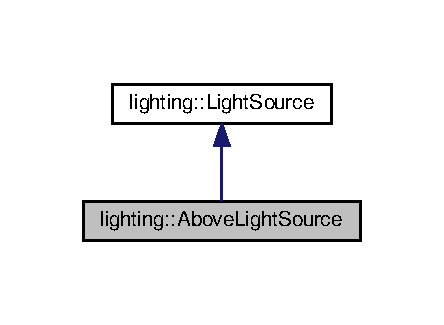
\includegraphics[width=213pt]{classlighting_1_1AboveLightSource__inherit__graph}
\end{center}
\end{figure}


Collaboration diagram for lighting\+:\+:Above\+Light\+Source\+:\nopagebreak
\begin{figure}[H]
\begin{center}
\leavevmode
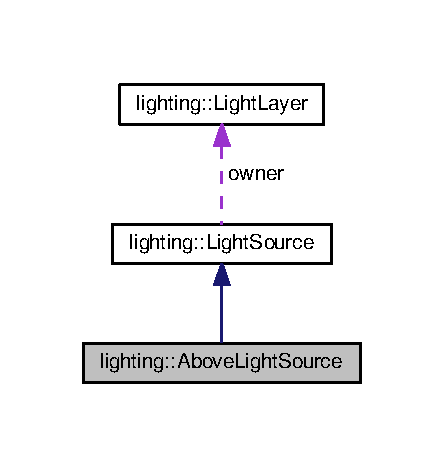
\includegraphics[width=213pt]{classlighting_1_1AboveLightSource__coll__graph}
\end{center}
\end{figure}
\subsection*{Public Member Functions}
\begin{DoxyCompactItemize}
\item 
\hyperlink{classlighting_1_1AboveLightSource_a0d155c74d7ce68008a17bff184d72db5}{Above\+Light\+Source} (\hyperlink{classlighting_1_1LightLayer}{Light\+Layer} $\ast$owner\+Light\+Layer, int \hyperlink{classlighting_1_1AboveLightSource_a558b3b3a03cdabc36a6ae73cbd41083d}{y\+Off}=0, uint8\+\_\+t r=\hyperlink{classlighting_1_1AboveLightSource_aa3134b6aa1f08719f50290094f014eb2}{D\+E\+F\+A\+U\+L\+T\+\_\+\+C\+O\+L\+O\+R\+\_\+\+V\+AL}, uint8\+\_\+t g=\hyperlink{classlighting_1_1AboveLightSource_aa3134b6aa1f08719f50290094f014eb2}{D\+E\+F\+A\+U\+L\+T\+\_\+\+C\+O\+L\+O\+R\+\_\+\+V\+AL}, uint8\+\_\+t b=\hyperlink{classlighting_1_1AboveLightSource_aa3134b6aa1f08719f50290094f014eb2}{D\+E\+F\+A\+U\+L\+T\+\_\+\+C\+O\+L\+O\+R\+\_\+\+V\+AL}, uint8\+\_\+t a=\hyperlink{classlighting_1_1AboveLightSource_aa3134b6aa1f08719f50290094f014eb2}{D\+E\+F\+A\+U\+L\+T\+\_\+\+C\+O\+L\+O\+R\+\_\+\+V\+AL})
\begin{DoxyCompactList}\small\item\em Initializes a new instance of the \hyperlink{classlighting_1_1AboveLightSource}{Above\+Light\+Source} class. Automatically adds itelf to {\itshape owner\+Light\+Layer} . \end{DoxyCompactList}\item 
void \hyperlink{classlighting_1_1AboveLightSource_a5a1e95ad0bc1ae4c4538f2899f46b37d}{set\+Light\+Color} (uint8\+\_\+t r, uint8\+\_\+t g, uint8\+\_\+t b, uint8\+\_\+t a)
\begin{DoxyCompactList}\small\item\em Sets \hyperlink{classlighting_1_1AboveLightSource_a67835e37619d5d86023ef1fbc315546b}{light\+Color}. \end{DoxyCompactList}\item 
virtual \hyperlink{classlighting_1_1AboveLightSource_a5f7e204332d81a44fbb2a89df03acfbd}{$\sim$\+Above\+Light\+Source} ()
\begin{DoxyCompactList}\small\item\em Finalizes an instance of the \hyperlink{classlighting_1_1AboveLightSource}{Above\+Light\+Source} class. Automatically removes itself from the \hyperlink{classlighting_1_1LightSource_ab991aac9d9ab3a1583f4acdc209055d5}{owner}. \end{DoxyCompactList}\end{DoxyCompactItemize}
\subsection*{Static Public Attributes}
\begin{DoxyCompactItemize}
\item 
static const uint8\+\_\+t \hyperlink{classlighting_1_1AboveLightSource_aa3134b6aa1f08719f50290094f014eb2}{D\+E\+F\+A\+U\+L\+T\+\_\+\+C\+O\+L\+O\+R\+\_\+\+V\+AL} = 180
\begin{DoxyCompactList}\small\item\em The default color code value for r, g, b, a \end{DoxyCompactList}\item 
static const int \hyperlink{classlighting_1_1AboveLightSource_aefd3bdb1bb3d0a20657812f75b23f8b2}{A\+B\+O\+V\+E\+\_\+\+L\+I\+G\+H\+T\+\_\+\+B\+L\+O\+C\+K\+E\+R\+\_\+Y} = -\/30
\begin{DoxyCompactList}\small\item\em The y value \hyperlink{classlighting_1_1AboveLightBlocker}{Above\+Light\+Blocker} will be added at. \end{DoxyCompactList}\item 
static const int \hyperlink{classlighting_1_1AboveLightSource_aa87131309853cc76a946de6e004aa778}{B\+O\+U\+N\+D\+\_\+\+O\+FF} = 400
\begin{DoxyCompactList}\small\item\em How far the bound points are from the screen. \end{DoxyCompactList}\item 
static const uint8\+\_\+t \hyperlink{classlighting_1_1AboveLightSource_a698c4d291629788288537b8d9c166132}{R\+A\+D\+I\+X\+\_\+\+B\+A\+S\+E\+\_\+\+B\+I\+TS} = 4
\begin{DoxyCompactList}\small\item\em The amount of bits in the radix base \end{DoxyCompactList}\item 
static const unsigned int \hyperlink{classlighting_1_1AboveLightSource_aa27d69b85b99509a937f3b6cf34e6f5b}{R\+A\+D\+I\+X\+\_\+\+B\+A\+S\+E\+\_\+\+N\+UM} = 16
\begin{DoxyCompactList}\small\item\em The max value of the radix base \end{DoxyCompactList}\item 
static const uint8\+\_\+t \hyperlink{classlighting_1_1AboveLightSource_a4154fa07c5a68055db8c6a710cf0dbec}{R\+A\+D\+I\+X\+\_\+\+M\+A\+X\+\_\+\+B\+I\+TS} = 16
\begin{DoxyCompactList}\small\item\em The maximum radix value in bits. \end{DoxyCompactList}\item 
static const unsigned int \hyperlink{classlighting_1_1AboveLightSource_afb7f4c5e212f5fcc97bcf06a16b21ac3}{R\+A\+D\+I\+X\+\_\+\+M\+A\+X\+\_\+\+N\+UM} = 65535
\begin{DoxyCompactList}\small\item\em The maximum value of the radix. \end{DoxyCompactList}\end{DoxyCompactItemize}
\subsection*{Protected Member Functions}
\begin{DoxyCompactItemize}
\item 
void \hyperlink{classlighting_1_1AboveLightSource_a40e7b34c807c7c91ff6889551a89ec88}{counting\+Sort\+Shade\+Points} (int bI)
\begin{DoxyCompactList}\small\item\em Countings the sort shade points. \end{DoxyCompactList}\item 
void \hyperlink{classlighting_1_1AboveLightSource_af874db3015b41b546bcc178d0904572a}{radix\+Sort\+Shade\+Points} ()
\begin{DoxyCompactList}\small\item\em Radixes the sort shade points based on their x-\/values. \end{DoxyCompactList}\item 
virtual void \hyperlink{classlighting_1_1AboveLightSource_a4b18ea492b7f63bc34f7bd269317c20e}{transfer\+Held\+Vars} () override
\begin{DoxyCompactList}\small\item\em Transfers the held vars. No implementation. \end{DoxyCompactList}\item 
virtual void \hyperlink{classlighting_1_1AboveLightSource_a13665ac64b61239624b430a49ab609ab}{create\+Shade\+Points} () override
\begin{DoxyCompactList}\small\item\em Populates \hyperlink{classlighting_1_1AboveLightSource_a255e98bb6aae0099178cb7aa2d9671a5}{shade\+Points} by using \hyperlink{classlighting_1_1LightSource_ab991aac9d9ab3a1583f4acdc209055d5}{owner}\textquotesingle{}s above\+Light\+Blockers and light\+Blockers. \end{DoxyCompactList}\item 
virtual void \hyperlink{classlighting_1_1AboveLightSource_a9331dd2674565685388ef044b71a4881}{map\+Shade\+Points} () override
\begin{DoxyCompactList}\small\item\em Processes the \hyperlink{classlighting_1_1AboveLightSource_a255e98bb6aae0099178cb7aa2d9671a5}{shade\+Points} and converts them to \hyperlink{classlighting_1_1AboveLightSource_a225b94f0f210561668b94e412c66443b}{draw\+Points}. \end{DoxyCompactList}\item 
virtual void \hyperlink{classlighting_1_1AboveLightSource_af858515032138900888d8db1a5f6812d}{draw\+Local} () override
\begin{DoxyCompactList}\small\item\em No body, there is no local drawing needed. \end{DoxyCompactList}\item 
virtual void \hyperlink{classlighting_1_1AboveLightSource_ae941abaa5da73f24c11d1e2c120af9ae}{draw\+To\+Light\+Map} () override
\begin{DoxyCompactList}\small\item\em Iterates through \hyperlink{classlighting_1_1AboveLightSource_a225b94f0f210561668b94e412c66443b}{draw\+Points} to draw to light\+Map. \end{DoxyCompactList}\item 
virtual void \hyperlink{classlighting_1_1AboveLightSource_a3625f4a181c5a2e78bc8549491e4e683}{create\+Bound\+Shade\+Points} ()
\begin{DoxyCompactList}\small\item\em Populates \hyperlink{classlighting_1_1AboveLightSource_a255e98bb6aae0099178cb7aa2d9671a5}{shade\+Points} with the boundary \hyperlink{classlighting_1_1AboveShadePoint}{Above\+Shade\+Point}s. \end{DoxyCompactList}\item 
virtual void \hyperlink{classlighting_1_1AboveLightSource_acc4e52dba4a3c64994b238f03b57df08}{reset\+Points} ()
\begin{DoxyCompactList}\small\item\em Clears and deletes elements in all point containers. \end{DoxyCompactList}\item 
virtual void \hyperlink{classlighting_1_1AboveLightSource_a86df533c28394981eb877e78fea594fb}{update\+Cast\+Points} (\hyperlink{classlighting_1_1AboveShadePoint}{Above\+Shade\+Point} $\ast$update\+Point)
\begin{DoxyCompactList}\small\item\em Updates the cast points. \end{DoxyCompactList}\item 
virtual bool \hyperlink{classlighting_1_1AboveLightSource_aa4fe1a6e9a19287417d66c911b98d0d0}{get\+Alpha\+Line\+AtX} (\hyperlink{classlighting_1_1AboveShadePoint}{Above\+Shade\+Point} $\ast$\&alpha\+Point, int \&i, float \&alpha\+ContactX, float \&alpha\+ContactY)
\begin{DoxyCompactList}\small\item\em Will iterate through all of the \hyperlink{classlighting_1_1ShadePoint}{Shade\+Point}s with the same x as the element in \hyperlink{classlighting_1_1AboveLightSource_a255e98bb6aae0099178cb7aa2d9671a5}{shade\+Points} at index {\itshape i}  and set the {\itshape alpha\+Point} , {\itshape alpha\+ContactX} , and {\itshape alpha\+ContactY}  to the point that has the minimum distance from the origin, and the highest angle between it and its connecting point. If a valid point is not found, return false and leave alpha\+Point, prevX, prevY as they were. \end{DoxyCompactList}\item 
virtual void \hyperlink{classlighting_1_1AboveLightSource_a43c39f611519c6f94a8a8a8165ed8a64}{handle\+First\+Shade\+Points} (\hyperlink{classlighting_1_1AboveShadePoint}{Above\+Shade\+Point} $\ast$\&alpha\+Point, float \&firstX, float \&firstY, int \&i)
\begin{DoxyCompactList}\small\item\em Handles the first shade points. \end{DoxyCompactList}\item 
virtual void \hyperlink{classlighting_1_1AboveLightSource_a4752f8d26b2d2584e79f5dbbe93f043d}{handle\+Last\+Shade\+Points} (\hyperlink{classlighting_1_1AboveShadePoint}{Above\+Shade\+Point} $\ast$alpha\+Point, float alpha\+ContactX, float alpha\+ContactY)
\begin{DoxyCompactList}\small\item\em Handles the last shade points. Currently no body. \end{DoxyCompactList}\item 
int \hyperlink{classlighting_1_1AboveLightSource_a113938f6773c454f6c36e553df6f1886}{get\+MinX} ()
\begin{DoxyCompactList}\small\item\em The minimum value of x for elements of \hyperlink{classlighting_1_1AboveLightSource_a255e98bb6aae0099178cb7aa2d9671a5}{shade\+Points}. \end{DoxyCompactList}\item 
int \hyperlink{classlighting_1_1AboveLightSource_a5818e15ade8eaaeb20ecb02c198e57bf}{get\+MaxX} ()
\begin{DoxyCompactList}\small\item\em The maximum value of x for elements of \hyperlink{classlighting_1_1AboveLightSource_a255e98bb6aae0099178cb7aa2d9671a5}{shade\+Points}. \end{DoxyCompactList}\item 
void {\bfseries add\+Draw\+Points} (float x1, float y1, float x2, float y2)\hypertarget{classlighting_1_1AboveLightSource_a926900f786af28265cac95751c3ce2ac}{}\label{classlighting_1_1AboveLightSource_a926900f786af28265cac95751c3ce2ac}

\item 
\hyperlink{classlighting_1_1AboveShadePoint}{Above\+Shade\+Point} $\ast$ \hyperlink{classlighting_1_1AboveLightSource_ac65260afb16ddd15ff49628168268cdb}{shadow\+Cast} (float x, float \&cY, \hyperlink{classlighting_1_1AboveShadePoint}{Above\+Shade\+Point} $\ast$exception\+Point=nullptr)
\begin{DoxyCompactList}\small\item\em Returns the line closest to the top of the screen at the given {\itshape x}  \end{DoxyCompactList}\end{DoxyCompactItemize}
\subsection*{Static Protected Member Functions}
\begin{DoxyCompactItemize}
\item 
static bool \hyperlink{classlighting_1_1AboveLightSource_a31861d0bb4bfa3a25e2f88b1662e0744}{Check\+Point\+Front} (\hyperlink{classlighting_1_1AboveShadePoint}{Above\+Shade\+Point} $\ast$alpha\+Point, \hyperlink{classlighting_1_1AboveShadePoint}{Above\+Shade\+Point} $\ast$check\+Point)
\begin{DoxyCompactList}\small\item\em Checks if {\itshape check\+Point}  is in front of the line created by alpha\+Point. \end{DoxyCompactList}\end{DoxyCompactItemize}
\subsection*{Protected Attributes}
\begin{DoxyCompactItemize}
\item 
int \hyperlink{classlighting_1_1AboveLightSource_a558b3b3a03cdabc36a6ae73cbd41083d}{y\+Off}
\begin{DoxyCompactList}\small\item\em Value added to the y-\/component of \hyperlink{classlighting_1_1AboveLightSource_a225b94f0f210561668b94e412c66443b}{draw\+Points}. \end{DoxyCompactList}\item 
std\+::vector$<$ float $>$ \hyperlink{classlighting_1_1AboveLightSource_a225b94f0f210561668b94e412c66443b}{draw\+Points}
\begin{DoxyCompactList}\small\item\em The coordinates of the points to draw. Even is x, odd is y. \end{DoxyCompactList}\item 
std\+::unordered\+\_\+set$<$ \hyperlink{classlighting_1_1AboveShadePoint}{Above\+Shade\+Point} $\ast$ $>$ \hyperlink{classlighting_1_1AboveLightSource_a59d73c54616c32422d4cbea6b981022e}{cast\+Points}
\begin{DoxyCompactList}\small\item\em Keeps track of the \hyperlink{classlighting_1_1AboveShadePoint}{Above\+Shade\+Point}s that can be shadow casted to. \end{DoxyCompactList}\item 
std\+::vector$<$ \hyperlink{classlighting_1_1AboveShadePoint}{Above\+Shade\+Point} $\ast$ $>$ \hyperlink{classlighting_1_1AboveLightSource_a255e98bb6aae0099178cb7aa2d9671a5}{shade\+Points}
\begin{DoxyCompactList}\small\item\em The \hyperlink{classlighting_1_1ShadePoint}{Shade\+Point}s created by \+::create\+Shade\+Points. \end{DoxyCompactList}\item 
A\+L\+L\+E\+G\+R\+O\+\_\+\+C\+O\+L\+OR \hyperlink{classlighting_1_1AboveLightSource_a67835e37619d5d86023ef1fbc315546b}{light\+Color}
\begin{DoxyCompactList}\small\item\em The color of the light. \end{DoxyCompactList}\end{DoxyCompactItemize}
\subsection*{Static Protected Attributes}
\begin{DoxyCompactItemize}
\item 
static const int \hyperlink{classlighting_1_1AboveLightSource_ac0d8f43e71b18876416b4091fb44bba6}{B\+O\+U\+N\+D\+\_\+\+P\+O\+I\+N\+T\+S\+\_\+\+S\+I\+ZE} = 2
\begin{DoxyCompactList}\small\item\em Amount of bound \hyperlink{classlighting_1_1AboveShadePoint}{Above\+Shade\+Point}s. \end{DoxyCompactList}\item 
static const int \hyperlink{classlighting_1_1AboveLightSource_a7f58e4685c32acd0c33f644b3578bcf4}{L\+I\+N\+E\+\_\+\+C\+H\+E\+C\+K\+\_\+\+O\+FF} = 2000
\begin{DoxyCompactList}\small\item\em When shadow\+Casting or checking points, this is how far off the y value is from the sceen to check for collisoins. \end{DoxyCompactList}\end{DoxyCompactItemize}
\subsection*{Friends}
\begin{DoxyCompactItemize}
\item 
class {\bfseries Light\+Layer}\hypertarget{classlighting_1_1AboveLightSource_aa4da5897890a726ecc5247c37419663b}{}\label{classlighting_1_1AboveLightSource_aa4da5897890a726ecc5247c37419663b}

\end{DoxyCompactItemize}
\subsection*{Additional Inherited Members}


\subsection{Detailed Description}
Represents the sun or any planetary source of light. Can be blocked by \hyperlink{classlighting_1_1AboveLightBlocker}{s or }s. 

\begin{DoxySeeAlso}{See also}
\hyperlink{classlighting_1_1LightSource}{Light\+Source}


\end{DoxySeeAlso}


\subsection{Constructor \& Destructor Documentation}
\index{lighting\+::\+Above\+Light\+Source@{lighting\+::\+Above\+Light\+Source}!Above\+Light\+Source@{Above\+Light\+Source}}
\index{Above\+Light\+Source@{Above\+Light\+Source}!lighting\+::\+Above\+Light\+Source@{lighting\+::\+Above\+Light\+Source}}
\subsubsection[{\texorpdfstring{Above\+Light\+Source(\+Light\+Layer $\ast$owner\+Light\+Layer, int y\+Off=0, uint8\+\_\+t r=\+D\+E\+F\+A\+U\+L\+T\+\_\+\+C\+O\+L\+O\+R\+\_\+\+V\+A\+L, uint8\+\_\+t g=\+D\+E\+F\+A\+U\+L\+T\+\_\+\+C\+O\+L\+O\+R\+\_\+\+V\+A\+L, uint8\+\_\+t b=\+D\+E\+F\+A\+U\+L\+T\+\_\+\+C\+O\+L\+O\+R\+\_\+\+V\+A\+L, uint8\+\_\+t a=\+D\+E\+F\+A\+U\+L\+T\+\_\+\+C\+O\+L\+O\+R\+\_\+\+V\+A\+L)}{AboveLightSource(LightLayer *ownerLightLayer, int yOff=0, uint8_t r=DEFAULT_COLOR_VAL, uint8_t g=DEFAULT_COLOR_VAL, uint8_t b=DEFAULT_COLOR_VAL, uint8_t a=DEFAULT_COLOR_VAL)}}]{\setlength{\rightskip}{0pt plus 5cm}lighting\+::\+Above\+Light\+Source\+::\+Above\+Light\+Source (
\begin{DoxyParamCaption}
\item[{{\bf Light\+Layer} $\ast$}]{owner\+Light\+Layer, }
\item[{int}]{y\+Off = {\ttfamily 0}, }
\item[{uint8\+\_\+t}]{r = {\ttfamily {\bf D\+E\+F\+A\+U\+L\+T\+\_\+\+C\+O\+L\+O\+R\+\_\+\+V\+AL}}, }
\item[{uint8\+\_\+t}]{g = {\ttfamily {\bf D\+E\+F\+A\+U\+L\+T\+\_\+\+C\+O\+L\+O\+R\+\_\+\+V\+AL}}, }
\item[{uint8\+\_\+t}]{b = {\ttfamily {\bf D\+E\+F\+A\+U\+L\+T\+\_\+\+C\+O\+L\+O\+R\+\_\+\+V\+AL}}, }
\item[{uint8\+\_\+t}]{a = {\ttfamily {\bf D\+E\+F\+A\+U\+L\+T\+\_\+\+C\+O\+L\+O\+R\+\_\+\+V\+AL}}}
\end{DoxyParamCaption}
)}\hypertarget{classlighting_1_1AboveLightSource_a0d155c74d7ce68008a17bff184d72db5}{}\label{classlighting_1_1AboveLightSource_a0d155c74d7ce68008a17bff184d72db5}


Initializes a new instance of the \hyperlink{classlighting_1_1AboveLightSource}{Above\+Light\+Source} class. Automatically adds itelf to {\itshape owner\+Light\+Layer} . 


\begin{DoxyParams}{Parameters}
{\em owner\+Light\+Layer} & The \hyperlink{classlighting_1_1LightLayer}{Light\+Layer} 
\begin{DoxyCode}
\textcolor{keyword}{this}
\end{DoxyCode}
 will be added to.\\
\hline
{\em y\+Off} & This value is added to the light y so the light can go further than the object it hit.\\
\hline
{\em r} & The red color value.\\
\hline
{\em g} & The green color value.\\
\hline
{\em b} & The blue color value.\\
\hline
{\em a} & a.\\
\hline
\end{DoxyParams}
\index{lighting\+::\+Above\+Light\+Source@{lighting\+::\+Above\+Light\+Source}!````~Above\+Light\+Source@{$\sim$\+Above\+Light\+Source}}
\index{````~Above\+Light\+Source@{$\sim$\+Above\+Light\+Source}!lighting\+::\+Above\+Light\+Source@{lighting\+::\+Above\+Light\+Source}}
\subsubsection[{\texorpdfstring{$\sim$\+Above\+Light\+Source()}{~AboveLightSource()}}]{\setlength{\rightskip}{0pt plus 5cm}lighting\+::\+Above\+Light\+Source\+::$\sim$\+Above\+Light\+Source (
\begin{DoxyParamCaption}
{}
\end{DoxyParamCaption}
)\hspace{0.3cm}{\ttfamily [virtual]}}\hypertarget{classlighting_1_1AboveLightSource_a5f7e204332d81a44fbb2a89df03acfbd}{}\label{classlighting_1_1AboveLightSource_a5f7e204332d81a44fbb2a89df03acfbd}


Finalizes an instance of the \hyperlink{classlighting_1_1AboveLightSource}{Above\+Light\+Source} class. Automatically removes itself from the \hyperlink{classlighting_1_1LightSource_ab991aac9d9ab3a1583f4acdc209055d5}{owner}. 



\subsection{Member Function Documentation}
\index{lighting\+::\+Above\+Light\+Source@{lighting\+::\+Above\+Light\+Source}!Check\+Point\+Front@{Check\+Point\+Front}}
\index{Check\+Point\+Front@{Check\+Point\+Front}!lighting\+::\+Above\+Light\+Source@{lighting\+::\+Above\+Light\+Source}}
\subsubsection[{\texorpdfstring{Check\+Point\+Front(\+Above\+Shade\+Point $\ast$alpha\+Point, Above\+Shade\+Point $\ast$check\+Point)}{CheckPointFront(AboveShadePoint *alphaPoint, AboveShadePoint *checkPoint)}}]{\setlength{\rightskip}{0pt plus 5cm}bool lighting\+::\+Above\+Light\+Source\+::\+Check\+Point\+Front (
\begin{DoxyParamCaption}
\item[{{\bf Above\+Shade\+Point} $\ast$}]{alpha\+Point, }
\item[{{\bf Above\+Shade\+Point} $\ast$}]{check\+Point}
\end{DoxyParamCaption}
)\hspace{0.3cm}{\ttfamily [static]}, {\ttfamily [protected]}}\hypertarget{classlighting_1_1AboveLightSource_a31861d0bb4bfa3a25e2f88b1662e0744}{}\label{classlighting_1_1AboveLightSource_a31861d0bb4bfa3a25e2f88b1662e0744}


Checks if {\itshape check\+Point}  is in front of the line created by alpha\+Point. 


\begin{DoxyParams}{Parameters}
{\em alpha\+Point} & One of the endpoints of the alpha line.\\
\hline
{\em check\+Point} & The point to check if in front of alpha line.\\
\hline
\end{DoxyParams}
\begin{DoxyReturn}{Returns}
If {\itshape check\+Point}  is in front of the line made by alpha\+Point.
\end{DoxyReturn}
\index{lighting\+::\+Above\+Light\+Source@{lighting\+::\+Above\+Light\+Source}!counting\+Sort\+Shade\+Points@{counting\+Sort\+Shade\+Points}}
\index{counting\+Sort\+Shade\+Points@{counting\+Sort\+Shade\+Points}!lighting\+::\+Above\+Light\+Source@{lighting\+::\+Above\+Light\+Source}}
\subsubsection[{\texorpdfstring{counting\+Sort\+Shade\+Points(int b\+I)}{countingSortShadePoints(int bI)}}]{\setlength{\rightskip}{0pt plus 5cm}void lighting\+::\+Above\+Light\+Source\+::counting\+Sort\+Shade\+Points (
\begin{DoxyParamCaption}
\item[{int}]{bI}
\end{DoxyParamCaption}
)\hspace{0.3cm}{\ttfamily [protected]}}\hypertarget{classlighting_1_1AboveLightSource_a40e7b34c807c7c91ff6889551a89ec88}{}\label{classlighting_1_1AboveLightSource_a40e7b34c807c7c91ff6889551a89ec88}


Countings the sort shade points. 


\begin{DoxyParams}{Parameters}
{\em bI} & The bits to shift by.\\
\hline
\end{DoxyParams}
\index{lighting\+::\+Above\+Light\+Source@{lighting\+::\+Above\+Light\+Source}!create\+Bound\+Shade\+Points@{create\+Bound\+Shade\+Points}}
\index{create\+Bound\+Shade\+Points@{create\+Bound\+Shade\+Points}!lighting\+::\+Above\+Light\+Source@{lighting\+::\+Above\+Light\+Source}}
\subsubsection[{\texorpdfstring{create\+Bound\+Shade\+Points()}{createBoundShadePoints()}}]{\setlength{\rightskip}{0pt plus 5cm}void lighting\+::\+Above\+Light\+Source\+::create\+Bound\+Shade\+Points (
\begin{DoxyParamCaption}
{}
\end{DoxyParamCaption}
)\hspace{0.3cm}{\ttfamily [protected]}, {\ttfamily [virtual]}}\hypertarget{classlighting_1_1AboveLightSource_a3625f4a181c5a2e78bc8549491e4e683}{}\label{classlighting_1_1AboveLightSource_a3625f4a181c5a2e78bc8549491e4e683}


Populates \hyperlink{classlighting_1_1AboveLightSource_a255e98bb6aae0099178cb7aa2d9671a5}{shade\+Points} with the boundary \hyperlink{classlighting_1_1AboveShadePoint}{Above\+Shade\+Point}s. 

\index{lighting\+::\+Above\+Light\+Source@{lighting\+::\+Above\+Light\+Source}!create\+Shade\+Points@{create\+Shade\+Points}}
\index{create\+Shade\+Points@{create\+Shade\+Points}!lighting\+::\+Above\+Light\+Source@{lighting\+::\+Above\+Light\+Source}}
\subsubsection[{\texorpdfstring{create\+Shade\+Points() override}{createShadePoints() override}}]{\setlength{\rightskip}{0pt plus 5cm}void lighting\+::\+Above\+Light\+Source\+::create\+Shade\+Points (
\begin{DoxyParamCaption}
{}
\end{DoxyParamCaption}
)\hspace{0.3cm}{\ttfamily [override]}, {\ttfamily [protected]}, {\ttfamily [virtual]}}\hypertarget{classlighting_1_1AboveLightSource_a13665ac64b61239624b430a49ab609ab}{}\label{classlighting_1_1AboveLightSource_a13665ac64b61239624b430a49ab609ab}


Populates \hyperlink{classlighting_1_1AboveLightSource_a255e98bb6aae0099178cb7aa2d9671a5}{shade\+Points} by using \hyperlink{classlighting_1_1LightSource_ab991aac9d9ab3a1583f4acdc209055d5}{owner}\textquotesingle{}s above\+Light\+Blockers and light\+Blockers. 



Implements \hyperlink{classlighting_1_1LightSource_a5bf73ee0586ba7620b917e57148d67be}{lighting\+::\+Light\+Source}.

\index{lighting\+::\+Above\+Light\+Source@{lighting\+::\+Above\+Light\+Source}!draw\+Local@{draw\+Local}}
\index{draw\+Local@{draw\+Local}!lighting\+::\+Above\+Light\+Source@{lighting\+::\+Above\+Light\+Source}}
\subsubsection[{\texorpdfstring{draw\+Local() override}{drawLocal() override}}]{\setlength{\rightskip}{0pt plus 5cm}virtual void lighting\+::\+Above\+Light\+Source\+::draw\+Local (
\begin{DoxyParamCaption}
{}
\end{DoxyParamCaption}
)\hspace{0.3cm}{\ttfamily [inline]}, {\ttfamily [override]}, {\ttfamily [protected]}, {\ttfamily [virtual]}}\hypertarget{classlighting_1_1AboveLightSource_af858515032138900888d8db1a5f6812d}{}\label{classlighting_1_1AboveLightSource_af858515032138900888d8db1a5f6812d}


No body, there is no local drawing needed. 



Implements \hyperlink{classlighting_1_1LightSource_ab15af06660d5cd4658d61ac2075aedea}{lighting\+::\+Light\+Source}.

\index{lighting\+::\+Above\+Light\+Source@{lighting\+::\+Above\+Light\+Source}!draw\+To\+Light\+Map@{draw\+To\+Light\+Map}}
\index{draw\+To\+Light\+Map@{draw\+To\+Light\+Map}!lighting\+::\+Above\+Light\+Source@{lighting\+::\+Above\+Light\+Source}}
\subsubsection[{\texorpdfstring{draw\+To\+Light\+Map() override}{drawToLightMap() override}}]{\setlength{\rightskip}{0pt plus 5cm}void lighting\+::\+Above\+Light\+Source\+::draw\+To\+Light\+Map (
\begin{DoxyParamCaption}
{}
\end{DoxyParamCaption}
)\hspace{0.3cm}{\ttfamily [override]}, {\ttfamily [protected]}, {\ttfamily [virtual]}}\hypertarget{classlighting_1_1AboveLightSource_ae941abaa5da73f24c11d1e2c120af9ae}{}\label{classlighting_1_1AboveLightSource_ae941abaa5da73f24c11d1e2c120af9ae}


Iterates through \hyperlink{classlighting_1_1AboveLightSource_a225b94f0f210561668b94e412c66443b}{draw\+Points} to draw to light\+Map. 



Implements \hyperlink{classlighting_1_1LightSource_a4e292cccdfb5784e97a1924ca00533b9}{lighting\+::\+Light\+Source}.

\index{lighting\+::\+Above\+Light\+Source@{lighting\+::\+Above\+Light\+Source}!get\+Alpha\+Line\+AtX@{get\+Alpha\+Line\+AtX}}
\index{get\+Alpha\+Line\+AtX@{get\+Alpha\+Line\+AtX}!lighting\+::\+Above\+Light\+Source@{lighting\+::\+Above\+Light\+Source}}
\subsubsection[{\texorpdfstring{get\+Alpha\+Line\+At\+X(\+Above\+Shade\+Point $\ast$\&alpha\+Point, int \&i, float \&alpha\+Contact\+X, float \&alpha\+Contact\+Y)}{getAlphaLineAtX(AboveShadePoint *&alphaPoint, int &i, float &alphaContactX, float &alphaContactY)}}]{\setlength{\rightskip}{0pt plus 5cm}bool lighting\+::\+Above\+Light\+Source\+::get\+Alpha\+Line\+AtX (
\begin{DoxyParamCaption}
\item[{{\bf Above\+Shade\+Point} $\ast$\&}]{alpha\+Point, }
\item[{int \&}]{i, }
\item[{float \&}]{alpha\+ContactX, }
\item[{float \&}]{alpha\+ContactY}
\end{DoxyParamCaption}
)\hspace{0.3cm}{\ttfamily [protected]}, {\ttfamily [virtual]}}\hypertarget{classlighting_1_1AboveLightSource_aa4fe1a6e9a19287417d66c911b98d0d0}{}\label{classlighting_1_1AboveLightSource_aa4fe1a6e9a19287417d66c911b98d0d0}


Will iterate through all of the \hyperlink{classlighting_1_1ShadePoint}{Shade\+Point}s with the same x as the element in \hyperlink{classlighting_1_1AboveLightSource_a255e98bb6aae0099178cb7aa2d9671a5}{shade\+Points} at index {\itshape i}  and set the {\itshape alpha\+Point} , {\itshape alpha\+ContactX} , and {\itshape alpha\+ContactY}  to the point that has the minimum distance from the origin, and the highest angle between it and its connecting point. If a valid point is not found, return false and leave alpha\+Point, prevX, prevY as they were. 


\begin{DoxyParams}{Parameters}
{\em alpha\+Point} & \hyperlink{classlighting_1_1ShadePoint}{Shade\+Point} represneting of the end points of the alpha\+Line.\\
\hline
{\em i} & The index of \hyperlink{classlighting_1_1AboveLightSource_a255e98bb6aae0099178cb7aa2d9671a5}{shade\+Points} with the x-\/value to check.\\
\hline
{\em alpha\+ContactX} & The last place an alpha\+Contact occured.\\
\hline
{\em alpha\+ContactY} & The last place an alpha\+Contact occureed.\\
\hline
\end{DoxyParams}
\begin{DoxyReturn}{Returns}

\end{DoxyReturn}
\index{lighting\+::\+Above\+Light\+Source@{lighting\+::\+Above\+Light\+Source}!get\+MaxX@{get\+MaxX}}
\index{get\+MaxX@{get\+MaxX}!lighting\+::\+Above\+Light\+Source@{lighting\+::\+Above\+Light\+Source}}
\subsubsection[{\texorpdfstring{get\+Max\+X()}{getMaxX()}}]{\setlength{\rightskip}{0pt plus 5cm}int lighting\+::\+Above\+Light\+Source\+::get\+MaxX (
\begin{DoxyParamCaption}
{}
\end{DoxyParamCaption}
)\hspace{0.3cm}{\ttfamily [protected]}}\hypertarget{classlighting_1_1AboveLightSource_a5818e15ade8eaaeb20ecb02c198e57bf}{}\label{classlighting_1_1AboveLightSource_a5818e15ade8eaaeb20ecb02c198e57bf}


The maximum value of x for elements of \hyperlink{classlighting_1_1AboveLightSource_a255e98bb6aae0099178cb7aa2d9671a5}{shade\+Points}. 

\begin{DoxyReturn}{Returns}

\end{DoxyReturn}
\index{lighting\+::\+Above\+Light\+Source@{lighting\+::\+Above\+Light\+Source}!get\+MinX@{get\+MinX}}
\index{get\+MinX@{get\+MinX}!lighting\+::\+Above\+Light\+Source@{lighting\+::\+Above\+Light\+Source}}
\subsubsection[{\texorpdfstring{get\+Min\+X()}{getMinX()}}]{\setlength{\rightskip}{0pt plus 5cm}int lighting\+::\+Above\+Light\+Source\+::get\+MinX (
\begin{DoxyParamCaption}
{}
\end{DoxyParamCaption}
)\hspace{0.3cm}{\ttfamily [inline]}, {\ttfamily [protected]}}\hypertarget{classlighting_1_1AboveLightSource_a113938f6773c454f6c36e553df6f1886}{}\label{classlighting_1_1AboveLightSource_a113938f6773c454f6c36e553df6f1886}


The minimum value of x for elements of \hyperlink{classlighting_1_1AboveLightSource_a255e98bb6aae0099178cb7aa2d9671a5}{shade\+Points}. 

\begin{DoxyReturn}{Returns}

\end{DoxyReturn}
\index{lighting\+::\+Above\+Light\+Source@{lighting\+::\+Above\+Light\+Source}!handle\+First\+Shade\+Points@{handle\+First\+Shade\+Points}}
\index{handle\+First\+Shade\+Points@{handle\+First\+Shade\+Points}!lighting\+::\+Above\+Light\+Source@{lighting\+::\+Above\+Light\+Source}}
\subsubsection[{\texorpdfstring{handle\+First\+Shade\+Points(\+Above\+Shade\+Point $\ast$\&alpha\+Point, float \&first\+X, float \&first\+Y, int \&i)}{handleFirstShadePoints(AboveShadePoint *&alphaPoint, float &firstX, float &firstY, int &i)}}]{\setlength{\rightskip}{0pt plus 5cm}void lighting\+::\+Above\+Light\+Source\+::handle\+First\+Shade\+Points (
\begin{DoxyParamCaption}
\item[{{\bf Above\+Shade\+Point} $\ast$\&}]{alpha\+Point, }
\item[{float \&}]{firstX, }
\item[{float \&}]{firstY, }
\item[{int \&}]{i}
\end{DoxyParamCaption}
)\hspace{0.3cm}{\ttfamily [protected]}, {\ttfamily [virtual]}}\hypertarget{classlighting_1_1AboveLightSource_a43c39f611519c6f94a8a8a8165ed8a64}{}\label{classlighting_1_1AboveLightSource_a43c39f611519c6f94a8a8a8165ed8a64}


Handles the first shade points. 


\begin{DoxyParams}{Parameters}
{\em alpha\+Point} & The alpha point.\\
\hline
{\em firstX} & The first x.\\
\hline
{\em firstY} & The first y.\\
\hline
{\em i} & The i.\\
\hline
\end{DoxyParams}
\index{lighting\+::\+Above\+Light\+Source@{lighting\+::\+Above\+Light\+Source}!handle\+Last\+Shade\+Points@{handle\+Last\+Shade\+Points}}
\index{handle\+Last\+Shade\+Points@{handle\+Last\+Shade\+Points}!lighting\+::\+Above\+Light\+Source@{lighting\+::\+Above\+Light\+Source}}
\subsubsection[{\texorpdfstring{handle\+Last\+Shade\+Points(\+Above\+Shade\+Point $\ast$alpha\+Point, float alpha\+Contact\+X, float alpha\+Contact\+Y)}{handleLastShadePoints(AboveShadePoint *alphaPoint, float alphaContactX, float alphaContactY)}}]{\setlength{\rightskip}{0pt plus 5cm}void lighting\+::\+Above\+Light\+Source\+::handle\+Last\+Shade\+Points (
\begin{DoxyParamCaption}
\item[{{\bf Above\+Shade\+Point} $\ast$}]{alpha\+Point, }
\item[{float}]{alpha\+ContactX, }
\item[{float}]{alpha\+ContactY}
\end{DoxyParamCaption}
)\hspace{0.3cm}{\ttfamily [protected]}, {\ttfamily [virtual]}}\hypertarget{classlighting_1_1AboveLightSource_a4752f8d26b2d2584e79f5dbbe93f043d}{}\label{classlighting_1_1AboveLightSource_a4752f8d26b2d2584e79f5dbbe93f043d}


Handles the last shade points. Currently no body. 


\begin{DoxyParams}{Parameters}
{\em alpha\+Point} & The alpha point.\\
\hline
{\em alpha\+ContactX} & The alpha contact x.\\
\hline
{\em alpha\+ContactY} & The alpha contact y.\\
\hline
\end{DoxyParams}
\index{lighting\+::\+Above\+Light\+Source@{lighting\+::\+Above\+Light\+Source}!map\+Shade\+Points@{map\+Shade\+Points}}
\index{map\+Shade\+Points@{map\+Shade\+Points}!lighting\+::\+Above\+Light\+Source@{lighting\+::\+Above\+Light\+Source}}
\subsubsection[{\texorpdfstring{map\+Shade\+Points() override}{mapShadePoints() override}}]{\setlength{\rightskip}{0pt plus 5cm}void lighting\+::\+Above\+Light\+Source\+::map\+Shade\+Points (
\begin{DoxyParamCaption}
{}
\end{DoxyParamCaption}
)\hspace{0.3cm}{\ttfamily [override]}, {\ttfamily [protected]}, {\ttfamily [virtual]}}\hypertarget{classlighting_1_1AboveLightSource_a9331dd2674565685388ef044b71a4881}{}\label{classlighting_1_1AboveLightSource_a9331dd2674565685388ef044b71a4881}


Processes the \hyperlink{classlighting_1_1AboveLightSource_a255e98bb6aae0099178cb7aa2d9671a5}{shade\+Points} and converts them to \hyperlink{classlighting_1_1AboveLightSource_a225b94f0f210561668b94e412c66443b}{draw\+Points}. 



Implements \hyperlink{classlighting_1_1LightSource_a5bbde61a54af327d43dc4afee751412c}{lighting\+::\+Light\+Source}.

\index{lighting\+::\+Above\+Light\+Source@{lighting\+::\+Above\+Light\+Source}!radix\+Sort\+Shade\+Points@{radix\+Sort\+Shade\+Points}}
\index{radix\+Sort\+Shade\+Points@{radix\+Sort\+Shade\+Points}!lighting\+::\+Above\+Light\+Source@{lighting\+::\+Above\+Light\+Source}}
\subsubsection[{\texorpdfstring{radix\+Sort\+Shade\+Points()}{radixSortShadePoints()}}]{\setlength{\rightskip}{0pt plus 5cm}void lighting\+::\+Above\+Light\+Source\+::radix\+Sort\+Shade\+Points (
\begin{DoxyParamCaption}
{}
\end{DoxyParamCaption}
)\hspace{0.3cm}{\ttfamily [protected]}}\hypertarget{classlighting_1_1AboveLightSource_af874db3015b41b546bcc178d0904572a}{}\label{classlighting_1_1AboveLightSource_af874db3015b41b546bcc178d0904572a}


Radixes the sort shade points based on their x-\/values. 

\index{lighting\+::\+Above\+Light\+Source@{lighting\+::\+Above\+Light\+Source}!reset\+Points@{reset\+Points}}
\index{reset\+Points@{reset\+Points}!lighting\+::\+Above\+Light\+Source@{lighting\+::\+Above\+Light\+Source}}
\subsubsection[{\texorpdfstring{reset\+Points()}{resetPoints()}}]{\setlength{\rightskip}{0pt plus 5cm}void lighting\+::\+Above\+Light\+Source\+::reset\+Points (
\begin{DoxyParamCaption}
{}
\end{DoxyParamCaption}
)\hspace{0.3cm}{\ttfamily [protected]}, {\ttfamily [virtual]}}\hypertarget{classlighting_1_1AboveLightSource_acc4e52dba4a3c64994b238f03b57df08}{}\label{classlighting_1_1AboveLightSource_acc4e52dba4a3c64994b238f03b57df08}


Clears and deletes elements in all point containers. 

\index{lighting\+::\+Above\+Light\+Source@{lighting\+::\+Above\+Light\+Source}!set\+Light\+Color@{set\+Light\+Color}}
\index{set\+Light\+Color@{set\+Light\+Color}!lighting\+::\+Above\+Light\+Source@{lighting\+::\+Above\+Light\+Source}}
\subsubsection[{\texorpdfstring{set\+Light\+Color(uint8\+\_\+t r, uint8\+\_\+t g, uint8\+\_\+t b, uint8\+\_\+t a)}{setLightColor(uint8_t r, uint8_t g, uint8_t b, uint8_t a)}}]{\setlength{\rightskip}{0pt plus 5cm}void lighting\+::\+Above\+Light\+Source\+::set\+Light\+Color (
\begin{DoxyParamCaption}
\item[{uint8\+\_\+t}]{r, }
\item[{uint8\+\_\+t}]{g, }
\item[{uint8\+\_\+t}]{b, }
\item[{uint8\+\_\+t}]{a}
\end{DoxyParamCaption}
)}\hypertarget{classlighting_1_1AboveLightSource_a5a1e95ad0bc1ae4c4538f2899f46b37d}{}\label{classlighting_1_1AboveLightSource_a5a1e95ad0bc1ae4c4538f2899f46b37d}


Sets \hyperlink{classlighting_1_1AboveLightSource_a67835e37619d5d86023ef1fbc315546b}{light\+Color}. 


\begin{DoxyParams}{Parameters}
{\em r} & The red color value.\\
\hline
{\em g} & The green color value.\\
\hline
{\em b} & The blue color value.\\
\hline
{\em a} & The alpha color value.\\
\hline
\end{DoxyParams}
\index{lighting\+::\+Above\+Light\+Source@{lighting\+::\+Above\+Light\+Source}!shadow\+Cast@{shadow\+Cast}}
\index{shadow\+Cast@{shadow\+Cast}!lighting\+::\+Above\+Light\+Source@{lighting\+::\+Above\+Light\+Source}}
\subsubsection[{\texorpdfstring{shadow\+Cast(float x, float \&c\+Y, Above\+Shade\+Point $\ast$exception\+Point=nullptr)}{shadowCast(float x, float &cY, AboveShadePoint *exceptionPoint=nullptr)}}]{\setlength{\rightskip}{0pt plus 5cm}{\bf Above\+Shade\+Point} $\ast$ lighting\+::\+Above\+Light\+Source\+::shadow\+Cast (
\begin{DoxyParamCaption}
\item[{float}]{x, }
\item[{float \&}]{cY, }
\item[{{\bf Above\+Shade\+Point} $\ast$}]{exception\+Point = {\ttfamily nullptr}}
\end{DoxyParamCaption}
)\hspace{0.3cm}{\ttfamily [protected]}}\hypertarget{classlighting_1_1AboveLightSource_ac65260afb16ddd15ff49628168268cdb}{}\label{classlighting_1_1AboveLightSource_ac65260afb16ddd15ff49628168268cdb}


Returns the line closest to the top of the screen at the given {\itshape x}  


\begin{DoxyParams}{Parameters}
{\em x} & The x.\\
\hline
{\em cY} & The contactY, output parameter.\\
\hline
{\em exception\+Point} & The exception point, will not be returned.\\
\hline
\end{DoxyParams}
\begin{DoxyReturn}{Returns}

\end{DoxyReturn}
\index{lighting\+::\+Above\+Light\+Source@{lighting\+::\+Above\+Light\+Source}!transfer\+Held\+Vars@{transfer\+Held\+Vars}}
\index{transfer\+Held\+Vars@{transfer\+Held\+Vars}!lighting\+::\+Above\+Light\+Source@{lighting\+::\+Above\+Light\+Source}}
\subsubsection[{\texorpdfstring{transfer\+Held\+Vars() override}{transferHeldVars() override}}]{\setlength{\rightskip}{0pt plus 5cm}virtual void lighting\+::\+Above\+Light\+Source\+::transfer\+Held\+Vars (
\begin{DoxyParamCaption}
{}
\end{DoxyParamCaption}
)\hspace{0.3cm}{\ttfamily [inline]}, {\ttfamily [override]}, {\ttfamily [protected]}, {\ttfamily [virtual]}}\hypertarget{classlighting_1_1AboveLightSource_a4b18ea492b7f63bc34f7bd269317c20e}{}\label{classlighting_1_1AboveLightSource_a4b18ea492b7f63bc34f7bd269317c20e}


Transfers the held vars. No implementation. 



Implements \hyperlink{classlighting_1_1LightSource_ae4be8445f78d1314e112aed9c25933fc}{lighting\+::\+Light\+Source}.

\index{lighting\+::\+Above\+Light\+Source@{lighting\+::\+Above\+Light\+Source}!update\+Cast\+Points@{update\+Cast\+Points}}
\index{update\+Cast\+Points@{update\+Cast\+Points}!lighting\+::\+Above\+Light\+Source@{lighting\+::\+Above\+Light\+Source}}
\subsubsection[{\texorpdfstring{update\+Cast\+Points(\+Above\+Shade\+Point $\ast$update\+Point)}{updateCastPoints(AboveShadePoint *updatePoint)}}]{\setlength{\rightskip}{0pt plus 5cm}void lighting\+::\+Above\+Light\+Source\+::update\+Cast\+Points (
\begin{DoxyParamCaption}
\item[{{\bf Above\+Shade\+Point} $\ast$}]{update\+Point}
\end{DoxyParamCaption}
)\hspace{0.3cm}{\ttfamily [protected]}, {\ttfamily [virtual]}}\hypertarget{classlighting_1_1AboveLightSource_a86df533c28394981eb877e78fea594fb}{}\label{classlighting_1_1AboveLightSource_a86df533c28394981eb877e78fea594fb}


Updates the cast points. 


\begin{DoxyParams}{Parameters}
{\em update\+Point} & The \hyperlink{classlighting_1_1AboveShadePoint}{Above\+Shade\+Point} to check if needing adding or removing from \hyperlink{classlighting_1_1AboveLightSource_a59d73c54616c32422d4cbea6b981022e}{cast\+Points}.\\
\hline
\end{DoxyParams}


\subsection{Member Data Documentation}
\index{lighting\+::\+Above\+Light\+Source@{lighting\+::\+Above\+Light\+Source}!A\+B\+O\+V\+E\+\_\+\+L\+I\+G\+H\+T\+\_\+\+B\+L\+O\+C\+K\+E\+R\+\_\+Y@{A\+B\+O\+V\+E\+\_\+\+L\+I\+G\+H\+T\+\_\+\+B\+L\+O\+C\+K\+E\+R\+\_\+Y}}
\index{A\+B\+O\+V\+E\+\_\+\+L\+I\+G\+H\+T\+\_\+\+B\+L\+O\+C\+K\+E\+R\+\_\+Y@{A\+B\+O\+V\+E\+\_\+\+L\+I\+G\+H\+T\+\_\+\+B\+L\+O\+C\+K\+E\+R\+\_\+Y}!lighting\+::\+Above\+Light\+Source@{lighting\+::\+Above\+Light\+Source}}
\subsubsection[{\texorpdfstring{A\+B\+O\+V\+E\+\_\+\+L\+I\+G\+H\+T\+\_\+\+B\+L\+O\+C\+K\+E\+R\+\_\+Y}{ABOVE_LIGHT_BLOCKER_Y}}]{\setlength{\rightskip}{0pt plus 5cm}const int lighting\+::\+Above\+Light\+Source\+::\+A\+B\+O\+V\+E\+\_\+\+L\+I\+G\+H\+T\+\_\+\+B\+L\+O\+C\+K\+E\+R\+\_\+Y = -\/30\hspace{0.3cm}{\ttfamily [static]}}\hypertarget{classlighting_1_1AboveLightSource_aefd3bdb1bb3d0a20657812f75b23f8b2}{}\label{classlighting_1_1AboveLightSource_aefd3bdb1bb3d0a20657812f75b23f8b2}


The y value \hyperlink{classlighting_1_1AboveLightBlocker}{Above\+Light\+Blocker} will be added at. 

\index{lighting\+::\+Above\+Light\+Source@{lighting\+::\+Above\+Light\+Source}!B\+O\+U\+N\+D\+\_\+\+O\+FF@{B\+O\+U\+N\+D\+\_\+\+O\+FF}}
\index{B\+O\+U\+N\+D\+\_\+\+O\+FF@{B\+O\+U\+N\+D\+\_\+\+O\+FF}!lighting\+::\+Above\+Light\+Source@{lighting\+::\+Above\+Light\+Source}}
\subsubsection[{\texorpdfstring{B\+O\+U\+N\+D\+\_\+\+O\+FF}{BOUND_OFF}}]{\setlength{\rightskip}{0pt plus 5cm}const int lighting\+::\+Above\+Light\+Source\+::\+B\+O\+U\+N\+D\+\_\+\+O\+FF = 400\hspace{0.3cm}{\ttfamily [static]}}\hypertarget{classlighting_1_1AboveLightSource_aa87131309853cc76a946de6e004aa778}{}\label{classlighting_1_1AboveLightSource_aa87131309853cc76a946de6e004aa778}


How far the bound points are from the screen. 

\index{lighting\+::\+Above\+Light\+Source@{lighting\+::\+Above\+Light\+Source}!B\+O\+U\+N\+D\+\_\+\+P\+O\+I\+N\+T\+S\+\_\+\+S\+I\+ZE@{B\+O\+U\+N\+D\+\_\+\+P\+O\+I\+N\+T\+S\+\_\+\+S\+I\+ZE}}
\index{B\+O\+U\+N\+D\+\_\+\+P\+O\+I\+N\+T\+S\+\_\+\+S\+I\+ZE@{B\+O\+U\+N\+D\+\_\+\+P\+O\+I\+N\+T\+S\+\_\+\+S\+I\+ZE}!lighting\+::\+Above\+Light\+Source@{lighting\+::\+Above\+Light\+Source}}
\subsubsection[{\texorpdfstring{B\+O\+U\+N\+D\+\_\+\+P\+O\+I\+N\+T\+S\+\_\+\+S\+I\+ZE}{BOUND_POINTS_SIZE}}]{\setlength{\rightskip}{0pt plus 5cm}const int lighting\+::\+Above\+Light\+Source\+::\+B\+O\+U\+N\+D\+\_\+\+P\+O\+I\+N\+T\+S\+\_\+\+S\+I\+ZE = 2\hspace{0.3cm}{\ttfamily [static]}, {\ttfamily [protected]}}\hypertarget{classlighting_1_1AboveLightSource_ac0d8f43e71b18876416b4091fb44bba6}{}\label{classlighting_1_1AboveLightSource_ac0d8f43e71b18876416b4091fb44bba6}


Amount of bound \hyperlink{classlighting_1_1AboveShadePoint}{Above\+Shade\+Point}s. 

\index{lighting\+::\+Above\+Light\+Source@{lighting\+::\+Above\+Light\+Source}!cast\+Points@{cast\+Points}}
\index{cast\+Points@{cast\+Points}!lighting\+::\+Above\+Light\+Source@{lighting\+::\+Above\+Light\+Source}}
\subsubsection[{\texorpdfstring{cast\+Points}{castPoints}}]{\setlength{\rightskip}{0pt plus 5cm}std\+::unordered\+\_\+set$<${\bf Above\+Shade\+Point}$\ast$$>$ lighting\+::\+Above\+Light\+Source\+::cast\+Points\hspace{0.3cm}{\ttfamily [protected]}}\hypertarget{classlighting_1_1AboveLightSource_a59d73c54616c32422d4cbea6b981022e}{}\label{classlighting_1_1AboveLightSource_a59d73c54616c32422d4cbea6b981022e}


Keeps track of the \hyperlink{classlighting_1_1AboveShadePoint}{Above\+Shade\+Point}s that can be shadow casted to. 

\index{lighting\+::\+Above\+Light\+Source@{lighting\+::\+Above\+Light\+Source}!D\+E\+F\+A\+U\+L\+T\+\_\+\+C\+O\+L\+O\+R\+\_\+\+V\+AL@{D\+E\+F\+A\+U\+L\+T\+\_\+\+C\+O\+L\+O\+R\+\_\+\+V\+AL}}
\index{D\+E\+F\+A\+U\+L\+T\+\_\+\+C\+O\+L\+O\+R\+\_\+\+V\+AL@{D\+E\+F\+A\+U\+L\+T\+\_\+\+C\+O\+L\+O\+R\+\_\+\+V\+AL}!lighting\+::\+Above\+Light\+Source@{lighting\+::\+Above\+Light\+Source}}
\subsubsection[{\texorpdfstring{D\+E\+F\+A\+U\+L\+T\+\_\+\+C\+O\+L\+O\+R\+\_\+\+V\+AL}{DEFAULT_COLOR_VAL}}]{\setlength{\rightskip}{0pt plus 5cm}const uint8\+\_\+t lighting\+::\+Above\+Light\+Source\+::\+D\+E\+F\+A\+U\+L\+T\+\_\+\+C\+O\+L\+O\+R\+\_\+\+V\+AL = 180\hspace{0.3cm}{\ttfamily [static]}}\hypertarget{classlighting_1_1AboveLightSource_aa3134b6aa1f08719f50290094f014eb2}{}\label{classlighting_1_1AboveLightSource_aa3134b6aa1f08719f50290094f014eb2}


The default color code value for r, g, b, a 

\index{lighting\+::\+Above\+Light\+Source@{lighting\+::\+Above\+Light\+Source}!draw\+Points@{draw\+Points}}
\index{draw\+Points@{draw\+Points}!lighting\+::\+Above\+Light\+Source@{lighting\+::\+Above\+Light\+Source}}
\subsubsection[{\texorpdfstring{draw\+Points}{drawPoints}}]{\setlength{\rightskip}{0pt plus 5cm}std\+::vector$<$float$>$ lighting\+::\+Above\+Light\+Source\+::draw\+Points\hspace{0.3cm}{\ttfamily [protected]}}\hypertarget{classlighting_1_1AboveLightSource_a225b94f0f210561668b94e412c66443b}{}\label{classlighting_1_1AboveLightSource_a225b94f0f210561668b94e412c66443b}


The coordinates of the points to draw. Even is x, odd is y. 

\index{lighting\+::\+Above\+Light\+Source@{lighting\+::\+Above\+Light\+Source}!light\+Color@{light\+Color}}
\index{light\+Color@{light\+Color}!lighting\+::\+Above\+Light\+Source@{lighting\+::\+Above\+Light\+Source}}
\subsubsection[{\texorpdfstring{light\+Color}{lightColor}}]{\setlength{\rightskip}{0pt plus 5cm}A\+L\+L\+E\+G\+R\+O\+\_\+\+C\+O\+L\+OR lighting\+::\+Above\+Light\+Source\+::light\+Color\hspace{0.3cm}{\ttfamily [protected]}}\hypertarget{classlighting_1_1AboveLightSource_a67835e37619d5d86023ef1fbc315546b}{}\label{classlighting_1_1AboveLightSource_a67835e37619d5d86023ef1fbc315546b}


The color of the light. 

\index{lighting\+::\+Above\+Light\+Source@{lighting\+::\+Above\+Light\+Source}!L\+I\+N\+E\+\_\+\+C\+H\+E\+C\+K\+\_\+\+O\+FF@{L\+I\+N\+E\+\_\+\+C\+H\+E\+C\+K\+\_\+\+O\+FF}}
\index{L\+I\+N\+E\+\_\+\+C\+H\+E\+C\+K\+\_\+\+O\+FF@{L\+I\+N\+E\+\_\+\+C\+H\+E\+C\+K\+\_\+\+O\+FF}!lighting\+::\+Above\+Light\+Source@{lighting\+::\+Above\+Light\+Source}}
\subsubsection[{\texorpdfstring{L\+I\+N\+E\+\_\+\+C\+H\+E\+C\+K\+\_\+\+O\+FF}{LINE_CHECK_OFF}}]{\setlength{\rightskip}{0pt plus 5cm}const int lighting\+::\+Above\+Light\+Source\+::\+L\+I\+N\+E\+\_\+\+C\+H\+E\+C\+K\+\_\+\+O\+FF = 2000\hspace{0.3cm}{\ttfamily [static]}, {\ttfamily [protected]}}\hypertarget{classlighting_1_1AboveLightSource_a7f58e4685c32acd0c33f644b3578bcf4}{}\label{classlighting_1_1AboveLightSource_a7f58e4685c32acd0c33f644b3578bcf4}


When shadow\+Casting or checking points, this is how far off the y value is from the sceen to check for collisoins. 

\index{lighting\+::\+Above\+Light\+Source@{lighting\+::\+Above\+Light\+Source}!R\+A\+D\+I\+X\+\_\+\+B\+A\+S\+E\+\_\+\+B\+I\+TS@{R\+A\+D\+I\+X\+\_\+\+B\+A\+S\+E\+\_\+\+B\+I\+TS}}
\index{R\+A\+D\+I\+X\+\_\+\+B\+A\+S\+E\+\_\+\+B\+I\+TS@{R\+A\+D\+I\+X\+\_\+\+B\+A\+S\+E\+\_\+\+B\+I\+TS}!lighting\+::\+Above\+Light\+Source@{lighting\+::\+Above\+Light\+Source}}
\subsubsection[{\texorpdfstring{R\+A\+D\+I\+X\+\_\+\+B\+A\+S\+E\+\_\+\+B\+I\+TS}{RADIX_BASE_BITS}}]{\setlength{\rightskip}{0pt plus 5cm}const uint8\+\_\+t lighting\+::\+Above\+Light\+Source\+::\+R\+A\+D\+I\+X\+\_\+\+B\+A\+S\+E\+\_\+\+B\+I\+TS = 4\hspace{0.3cm}{\ttfamily [static]}}\hypertarget{classlighting_1_1AboveLightSource_a698c4d291629788288537b8d9c166132}{}\label{classlighting_1_1AboveLightSource_a698c4d291629788288537b8d9c166132}


The amount of bits in the radix base 

\index{lighting\+::\+Above\+Light\+Source@{lighting\+::\+Above\+Light\+Source}!R\+A\+D\+I\+X\+\_\+\+B\+A\+S\+E\+\_\+\+N\+UM@{R\+A\+D\+I\+X\+\_\+\+B\+A\+S\+E\+\_\+\+N\+UM}}
\index{R\+A\+D\+I\+X\+\_\+\+B\+A\+S\+E\+\_\+\+N\+UM@{R\+A\+D\+I\+X\+\_\+\+B\+A\+S\+E\+\_\+\+N\+UM}!lighting\+::\+Above\+Light\+Source@{lighting\+::\+Above\+Light\+Source}}
\subsubsection[{\texorpdfstring{R\+A\+D\+I\+X\+\_\+\+B\+A\+S\+E\+\_\+\+N\+UM}{RADIX_BASE_NUM}}]{\setlength{\rightskip}{0pt plus 5cm}const unsigned int lighting\+::\+Above\+Light\+Source\+::\+R\+A\+D\+I\+X\+\_\+\+B\+A\+S\+E\+\_\+\+N\+UM = 16\hspace{0.3cm}{\ttfamily [static]}}\hypertarget{classlighting_1_1AboveLightSource_aa27d69b85b99509a937f3b6cf34e6f5b}{}\label{classlighting_1_1AboveLightSource_aa27d69b85b99509a937f3b6cf34e6f5b}


The max value of the radix base 

\index{lighting\+::\+Above\+Light\+Source@{lighting\+::\+Above\+Light\+Source}!R\+A\+D\+I\+X\+\_\+\+M\+A\+X\+\_\+\+B\+I\+TS@{R\+A\+D\+I\+X\+\_\+\+M\+A\+X\+\_\+\+B\+I\+TS}}
\index{R\+A\+D\+I\+X\+\_\+\+M\+A\+X\+\_\+\+B\+I\+TS@{R\+A\+D\+I\+X\+\_\+\+M\+A\+X\+\_\+\+B\+I\+TS}!lighting\+::\+Above\+Light\+Source@{lighting\+::\+Above\+Light\+Source}}
\subsubsection[{\texorpdfstring{R\+A\+D\+I\+X\+\_\+\+M\+A\+X\+\_\+\+B\+I\+TS}{RADIX_MAX_BITS}}]{\setlength{\rightskip}{0pt plus 5cm}const uint8\+\_\+t lighting\+::\+Above\+Light\+Source\+::\+R\+A\+D\+I\+X\+\_\+\+M\+A\+X\+\_\+\+B\+I\+TS = 16\hspace{0.3cm}{\ttfamily [static]}}\hypertarget{classlighting_1_1AboveLightSource_a4154fa07c5a68055db8c6a710cf0dbec}{}\label{classlighting_1_1AboveLightSource_a4154fa07c5a68055db8c6a710cf0dbec}


The maximum radix value in bits. 

\index{lighting\+::\+Above\+Light\+Source@{lighting\+::\+Above\+Light\+Source}!R\+A\+D\+I\+X\+\_\+\+M\+A\+X\+\_\+\+N\+UM@{R\+A\+D\+I\+X\+\_\+\+M\+A\+X\+\_\+\+N\+UM}}
\index{R\+A\+D\+I\+X\+\_\+\+M\+A\+X\+\_\+\+N\+UM@{R\+A\+D\+I\+X\+\_\+\+M\+A\+X\+\_\+\+N\+UM}!lighting\+::\+Above\+Light\+Source@{lighting\+::\+Above\+Light\+Source}}
\subsubsection[{\texorpdfstring{R\+A\+D\+I\+X\+\_\+\+M\+A\+X\+\_\+\+N\+UM}{RADIX_MAX_NUM}}]{\setlength{\rightskip}{0pt plus 5cm}const unsigned int lighting\+::\+Above\+Light\+Source\+::\+R\+A\+D\+I\+X\+\_\+\+M\+A\+X\+\_\+\+N\+UM = 65535\hspace{0.3cm}{\ttfamily [static]}}\hypertarget{classlighting_1_1AboveLightSource_afb7f4c5e212f5fcc97bcf06a16b21ac3}{}\label{classlighting_1_1AboveLightSource_afb7f4c5e212f5fcc97bcf06a16b21ac3}


The maximum value of the radix. 

\index{lighting\+::\+Above\+Light\+Source@{lighting\+::\+Above\+Light\+Source}!shade\+Points@{shade\+Points}}
\index{shade\+Points@{shade\+Points}!lighting\+::\+Above\+Light\+Source@{lighting\+::\+Above\+Light\+Source}}
\subsubsection[{\texorpdfstring{shade\+Points}{shadePoints}}]{\setlength{\rightskip}{0pt plus 5cm}std\+::vector$<${\bf Above\+Shade\+Point}$\ast$$>$ lighting\+::\+Above\+Light\+Source\+::shade\+Points\hspace{0.3cm}{\ttfamily [protected]}}\hypertarget{classlighting_1_1AboveLightSource_a255e98bb6aae0099178cb7aa2d9671a5}{}\label{classlighting_1_1AboveLightSource_a255e98bb6aae0099178cb7aa2d9671a5}


The \hyperlink{classlighting_1_1ShadePoint}{Shade\+Point}s created by \+::create\+Shade\+Points. 

\index{lighting\+::\+Above\+Light\+Source@{lighting\+::\+Above\+Light\+Source}!y\+Off@{y\+Off}}
\index{y\+Off@{y\+Off}!lighting\+::\+Above\+Light\+Source@{lighting\+::\+Above\+Light\+Source}}
\subsubsection[{\texorpdfstring{y\+Off}{yOff}}]{\setlength{\rightskip}{0pt plus 5cm}int lighting\+::\+Above\+Light\+Source\+::y\+Off\hspace{0.3cm}{\ttfamily [protected]}}\hypertarget{classlighting_1_1AboveLightSource_a558b3b3a03cdabc36a6ae73cbd41083d}{}\label{classlighting_1_1AboveLightSource_a558b3b3a03cdabc36a6ae73cbd41083d}


Value added to the y-\/component of \hyperlink{classlighting_1_1AboveLightSource_a225b94f0f210561668b94e412c66443b}{draw\+Points}. 



The documentation for this class was generated from the following files\+:\begin{DoxyCompactItemize}
\item 
Above\+Light\+Source.\+h\item 
Above\+Light\+Source.\+cpp\end{DoxyCompactItemize}

\hypertarget{classlighting_1_1AboveShadePoint}{}\section{lighting\+:\+:Above\+Shade\+Point Class Reference}
\label{classlighting_1_1AboveShadePoint}\index{lighting\+::\+Above\+Shade\+Point@{lighting\+::\+Above\+Shade\+Point}}


Variant of \hyperlink{classlighting_1_1ShadePoint}{Shade\+Point} made for \hyperlink{classlighting_1_1AboveLightSource}{Above\+Light\+Source}s.  




{\ttfamily \#include $<$Above\+Shade\+Point.\+h$>$}



Inheritance diagram for lighting\+:\+:Above\+Shade\+Point\+:\nopagebreak
\begin{figure}[H]
\begin{center}
\leavevmode
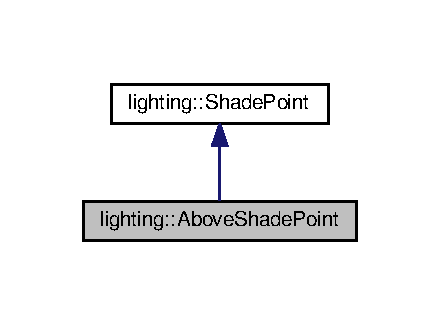
\includegraphics[width=211pt]{classlighting_1_1AboveShadePoint__inherit__graph}
\end{center}
\end{figure}


Collaboration diagram for lighting\+:\+:Above\+Shade\+Point\+:\nopagebreak
\begin{figure}[H]
\begin{center}
\leavevmode
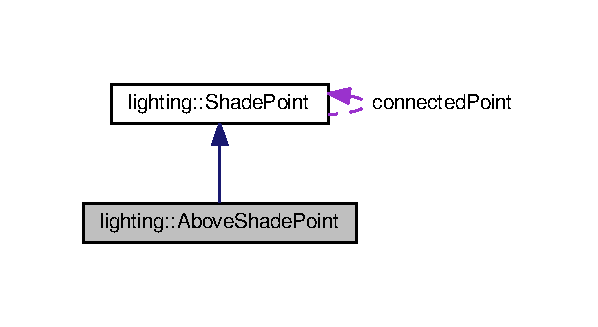
\includegraphics[width=287pt]{classlighting_1_1AboveShadePoint__coll__graph}
\end{center}
\end{figure}
\subsection*{Public Member Functions}
\begin{DoxyCompactItemize}
\item 
\hyperlink{classlighting_1_1AboveShadePoint_a13dcc1328ba52890bb23ecdb96b41de2}{Above\+Shade\+Point} (float \hyperlink{classlighting_1_1ShadePoint_a087db3eacccf6731f674f123c22400ec}{x}, float \hyperlink{classlighting_1_1ShadePoint_a427350496a448f0dd7424955a6c21ea2}{y}, int minX, int maxX)
\begin{DoxyCompactList}\small\item\em Initializes a new instance of the \hyperlink{classlighting_1_1AboveShadePoint}{Above\+Shade\+Point} class. Sets the position and the radix\+Val. \end{DoxyCompactList}\item 
\hyperlink{classlighting_1_1AboveShadePoint}{Above\+Shade\+Point} $\ast$ \hyperlink{classlighting_1_1AboveShadePoint_a68d9e7274fcc10333d16f259ae87a360}{get\+Connect\+Point} ()
\begin{DoxyCompactList}\small\item\em Gets the \hyperlink{classlighting_1_1ShadePoint_a0840495febcd385a90e89e003aa15972}{connected\+Point} which represents the other endpoint of the line. \end{DoxyCompactList}\item 
\hyperlink{classlighting_1_1AboveShadePoint_ad699ddbcdfea524594160f19021e7c2d}{$\sim$\+Above\+Shade\+Point} ()
\begin{DoxyCompactList}\small\item\em Finalizes an instance of the \hyperlink{classlighting_1_1AboveShadePoint}{Above\+Shade\+Point} class. \end{DoxyCompactList}\end{DoxyCompactItemize}
\subsection*{Public Attributes}
\begin{DoxyCompactItemize}
\item 
unsigned int {\bfseries radix\+Val}\hypertarget{classlighting_1_1AboveShadePoint_afeebe59ac2c4bce6a105e71a390c11a9}{}\label{classlighting_1_1AboveShadePoint_afeebe59ac2c4bce6a105e71a390c11a9}

\end{DoxyCompactItemize}
\subsection*{Additional Inherited Members}


\subsection{Detailed Description}
Variant of \hyperlink{classlighting_1_1ShadePoint}{Shade\+Point} made for \hyperlink{classlighting_1_1AboveLightSource}{Above\+Light\+Source}s. 

\begin{DoxySeeAlso}{See also}
\hyperlink{classlighting_1_1ShadePoint}{Shade\+Point}


\end{DoxySeeAlso}


\subsection{Constructor \& Destructor Documentation}
\index{lighting\+::\+Above\+Shade\+Point@{lighting\+::\+Above\+Shade\+Point}!Above\+Shade\+Point@{Above\+Shade\+Point}}
\index{Above\+Shade\+Point@{Above\+Shade\+Point}!lighting\+::\+Above\+Shade\+Point@{lighting\+::\+Above\+Shade\+Point}}
\subsubsection[{\texorpdfstring{Above\+Shade\+Point(float x, float y, int min\+X, int max\+X)}{AboveShadePoint(float x, float y, int minX, int maxX)}}]{\setlength{\rightskip}{0pt plus 5cm}lighting\+::\+Above\+Shade\+Point\+::\+Above\+Shade\+Point (
\begin{DoxyParamCaption}
\item[{float}]{x, }
\item[{float}]{y, }
\item[{int}]{minX, }
\item[{int}]{maxX}
\end{DoxyParamCaption}
)}\hypertarget{classlighting_1_1AboveShadePoint_a13dcc1328ba52890bb23ecdb96b41de2}{}\label{classlighting_1_1AboveShadePoint_a13dcc1328ba52890bb23ecdb96b41de2}


Initializes a new instance of the \hyperlink{classlighting_1_1AboveShadePoint}{Above\+Shade\+Point} class. Sets the position and the radix\+Val. 


\begin{DoxyParams}{Parameters}
{\em x} & The horizontal position.\\
\hline
{\em y} & The vertical position.\\
\hline
{\em maxX} & The maximum value for {\itshape x} , used to set radix\+Val.\\
\hline
\end{DoxyParams}
\index{lighting\+::\+Above\+Shade\+Point@{lighting\+::\+Above\+Shade\+Point}!````~Above\+Shade\+Point@{$\sim$\+Above\+Shade\+Point}}
\index{````~Above\+Shade\+Point@{$\sim$\+Above\+Shade\+Point}!lighting\+::\+Above\+Shade\+Point@{lighting\+::\+Above\+Shade\+Point}}
\subsubsection[{\texorpdfstring{$\sim$\+Above\+Shade\+Point()}{~AboveShadePoint()}}]{\setlength{\rightskip}{0pt plus 5cm}lighting\+::\+Above\+Shade\+Point\+::$\sim$\+Above\+Shade\+Point (
\begin{DoxyParamCaption}
{}
\end{DoxyParamCaption}
)}\hypertarget{classlighting_1_1AboveShadePoint_ad699ddbcdfea524594160f19021e7c2d}{}\label{classlighting_1_1AboveShadePoint_ad699ddbcdfea524594160f19021e7c2d}


Finalizes an instance of the \hyperlink{classlighting_1_1AboveShadePoint}{Above\+Shade\+Point} class. 



\subsection{Member Function Documentation}
\index{lighting\+::\+Above\+Shade\+Point@{lighting\+::\+Above\+Shade\+Point}!get\+Connect\+Point@{get\+Connect\+Point}}
\index{get\+Connect\+Point@{get\+Connect\+Point}!lighting\+::\+Above\+Shade\+Point@{lighting\+::\+Above\+Shade\+Point}}
\subsubsection[{\texorpdfstring{get\+Connect\+Point()}{getConnectPoint()}}]{\setlength{\rightskip}{0pt plus 5cm}{\bf Above\+Shade\+Point}$\ast$ lighting\+::\+Above\+Shade\+Point\+::get\+Connect\+Point (
\begin{DoxyParamCaption}
{}
\end{DoxyParamCaption}
)\hspace{0.3cm}{\ttfamily [inline]}}\hypertarget{classlighting_1_1AboveShadePoint_a68d9e7274fcc10333d16f259ae87a360}{}\label{classlighting_1_1AboveShadePoint_a68d9e7274fcc10333d16f259ae87a360}


Gets the \hyperlink{classlighting_1_1ShadePoint_a0840495febcd385a90e89e003aa15972}{connected\+Point} which represents the other endpoint of the line. 

\begin{DoxyReturn}{Returns}

\end{DoxyReturn}


The documentation for this class was generated from the following files\+:\begin{DoxyCompactItemize}
\item 
Above\+Shade\+Point.\+h\item 
Above\+Shade\+Point.\+cpp\end{DoxyCompactItemize}

\hypertarget{classlighting_1_1CircleLightSource}{}\section{lighting\+:\+:Circle\+Light\+Source Class Reference}
\label{classlighting_1_1CircleLightSource}\index{lighting\+::\+Circle\+Light\+Source@{lighting\+::\+Circle\+Light\+Source}}


A child of \hyperlink{classlighting_1_1LightSource}{Light\+Source} represents a full circle of light that would be produced by an oil lamp or a light bulb.  




{\ttfamily \#include $<$Circle\+Light\+Source.\+h$>$}



Inheritance diagram for lighting\+:\+:Circle\+Light\+Source\+:\nopagebreak
\begin{figure}[H]
\begin{center}
\leavevmode
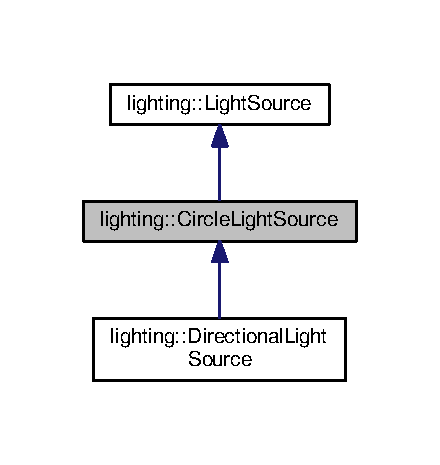
\includegraphics[width=211pt]{classlighting_1_1CircleLightSource__inherit__graph}
\end{center}
\end{figure}


Collaboration diagram for lighting\+:\+:Circle\+Light\+Source\+:\nopagebreak
\begin{figure}[H]
\begin{center}
\leavevmode
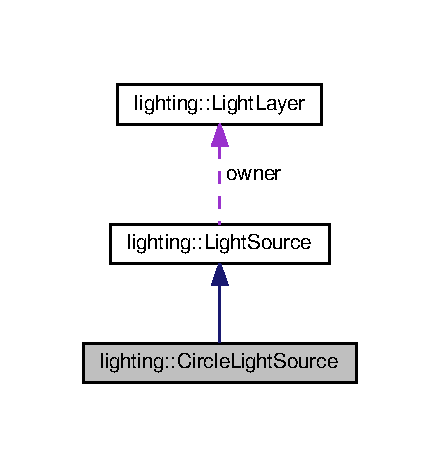
\includegraphics[width=211pt]{classlighting_1_1CircleLightSource__coll__graph}
\end{center}
\end{figure}
\subsection*{Public Member Functions}
\begin{DoxyCompactItemize}
\item 
\hyperlink{classlighting_1_1CircleLightSource_ade3ca945a040132851a26bef3c22fe6e}{Circle\+Light\+Source} (\hyperlink{classlighting_1_1LightLayer}{Light\+Layer} $\ast$owner\+Light\+Layer, float \hyperlink{classlighting_1_1CircleLightSource_a4da9b32f524563c2faeba5ea81dfe6fb}{radius}, uint8\+\_\+t r=U\+I\+N\+T8\+\_\+\+M\+AX, uint8\+\_\+t g=U\+I\+N\+T8\+\_\+\+M\+AX, uint8\+\_\+t b=U\+I\+N\+T8\+\_\+\+M\+AX)
\begin{DoxyCompactList}\small\item\em Initializes a new instance of the \hyperlink{classlighting_1_1CircleLightSource}{Circle\+Light\+Source} class. Automatically adds itself to the {\itshape owner\+Light\+Layer} . \end{DoxyCompactList}\item 
void \hyperlink{classlighting_1_1CircleLightSource_ae035f07aeb1e540c6066a4ff82bf4b54}{set\+XY} (float \hyperlink{classlighting_1_1CircleLightSource_afd27de5d967e2a308dadeff29d3c2883}{x}, float \hyperlink{classlighting_1_1CircleLightSource_ac05186b92c9bdfcef8a27cc89f8c9b52}{y})
\begin{DoxyCompactList}\small\item\em Sets the horizontal and vertical position of the center of the \hyperlink{classlighting_1_1CircleLightSource}{Circle\+Light\+Source} on the screen. Values are stored in \hyperlink{classlighting_1_1CircleLightSource_aa008d846fd893f0ff40e5994af4d487e}{heldX} and heldY until \hyperlink{classlighting_1_1CircleLightSource_afc39570a33c19b17fb8153be592b01e9}{transfer\+Held\+Vars()} is called. \end{DoxyCompactList}\item 
virtual void \hyperlink{classlighting_1_1CircleLightSource_a8ca70332ba3b1926e6c65a56cb30416c}{set\+Light\+Color} (uint8\+\_\+t r, uint8\+\_\+t g, uint8\+\_\+t b)
\begin{DoxyCompactList}\small\item\em Sets the color of the light. Modifier for \hyperlink{classlighting_1_1CircleLightSource_a39d1b9f5bfb54facf6a7e36ed0ffda82}{light\+Color}. \end{DoxyCompactList}\end{DoxyCompactItemize}
\subsection*{Static Public Attributes}
\begin{DoxyCompactItemize}
\item 
static uint64\+\_\+t {\bfseries Shade\+Points\+Processed} = 0\hypertarget{classlighting_1_1CircleLightSource_ac5ee6f2194afd0dfd04470ca554d7c3a}{}\label{classlighting_1_1CircleLightSource_ac5ee6f2194afd0dfd04470ca554d7c3a}

\item 
static uint64\+\_\+t {\bfseries Shadow\+Called} = 0\hypertarget{classlighting_1_1CircleLightSource_a9ad414cfb620c9253fbda3d6a9b89f50}{}\label{classlighting_1_1CircleLightSource_a9ad414cfb620c9253fbda3d6a9b89f50}

\item 
static uint64\+\_\+t {\bfseries Cast\+Points\+Processed} = 0\hypertarget{classlighting_1_1CircleLightSource_aee2dd14e70c371618e6d7161b2e8187e}{}\label{classlighting_1_1CircleLightSource_aee2dd14e70c371618e6d7161b2e8187e}

\item 
static uint64\+\_\+t {\bfseries Total\+Cycles} = 0\hypertarget{classlighting_1_1CircleLightSource_ada2d8673056053ec59ce2053eb691e0a}{}\label{classlighting_1_1CircleLightSource_ada2d8673056053ec59ce2053eb691e0a}

\item 
static const uint8\+\_\+t \hyperlink{classlighting_1_1CircleLightSource_a94be83c3a3e575b5670ec6c6abe8a6e7}{R\+A\+D\+I\+X\+\_\+\+B\+A\+S\+E\+\_\+\+B\+I\+TS} = 4
\begin{DoxyCompactList}\small\item\em Number of bits for the radix base \end{DoxyCompactList}\item 
static const unsigned int {\bfseries R\+A\+D\+I\+X\+\_\+\+B\+A\+S\+E\+\_\+\+N\+UM} = 16\hypertarget{classlighting_1_1CircleLightSource_afa4c65f061bb4201a36aa7feee13b4c0}{}\label{classlighting_1_1CircleLightSource_afa4c65f061bb4201a36aa7feee13b4c0}

\item 
static const uint8\+\_\+t \hyperlink{classlighting_1_1CircleLightSource_a9a4d058eac85eeb8c542abd69069e4b2}{R\+A\+D\+I\+X\+\_\+\+M\+A\+X\+\_\+\+B\+I\+TS} = 32
\begin{DoxyCompactList}\small\item\em Number of bits for the maximum value of elements sorted by radix sort \end{DoxyCompactList}\item 
static unsigned int {\bfseries R\+A\+D\+I\+X\+\_\+\+M\+A\+X\+\_\+\+N\+UM} = pow(2, 32) -\/ 1\hypertarget{classlighting_1_1CircleLightSource_adaa12ee54e0cecf9691061646b7e71f4}{}\label{classlighting_1_1CircleLightSource_adaa12ee54e0cecf9691061646b7e71f4}

\item 
static const float \hyperlink{classlighting_1_1CircleLightSource_a139a7246edba5531259b778ce0ca79b3}{M\+A\+X\+\_\+\+N\+E\+G\+\_\+\+F\+L\+O\+AT} = -\/std\+::numeric\+\_\+limits$<$float$>$\+::max()
\begin{DoxyCompactList}\small\item\em Set to the most negative possible value of float \end{DoxyCompactList}\end{DoxyCompactItemize}
\subsection*{Protected Member Functions}
\begin{DoxyCompactItemize}
\item 
void \hyperlink{classlighting_1_1CircleLightSource_a850ea8b5a1480473bd40a82a9687f229}{radix\+Sort\+Shade\+Points} ()
\begin{DoxyCompactList}\small\item\em Uses radix sort to sort the elements of \hyperlink{classlighting_1_1CircleLightSource_acdfea64be9d142f669338c5e206e753e}{shade\+Points}. \end{DoxyCompactList}\item 
void \hyperlink{classlighting_1_1CircleLightSource_ac7cbab4f6a38d8359a2637a875427e75}{counting\+Sort\+Shade\+Points} (int bI)
\begin{DoxyCompactList}\small\item\em Called by \hyperlink{classlighting_1_1CircleLightSource_a850ea8b5a1480473bd40a82a9687f229}{radix\+Sort\+Shade\+Points} as a helper method for the sorting process \end{DoxyCompactList}\item 
virtual void \hyperlink{classlighting_1_1CircleLightSource_afc39570a33c19b17fb8153be592b01e9}{transfer\+Held\+Vars} () override
\begin{DoxyCompactList}\small\item\em Sets the ,  attributes to the corresponding \char`\"{}held\char`\"{} attributes. Called from Light\+Layer\+::dispatch(). \end{DoxyCompactList}\item 
virtual void \hyperlink{classlighting_1_1CircleLightSource_aaa80bb9a9a27f3c74bf86cfd547d5f36}{create\+Shade\+Points} () override
\begin{DoxyCompactList}\small\item\em Converts all elements of {\itshape light\+Blockers}  into two \hyperlink{classlighting_1_1CircleShadePoint}{Circle\+Shade\+Point}s which are stored in the \hyperlink{classlighting_1_1CircleLightSource_acdfea64be9d142f669338c5e206e753e}{shade\+Points} vector and then sorted using \+::radix\+Sort\+Shade\+Points. Function also handles edge cases. \end{DoxyCompactList}\item 
virtual void \hyperlink{classlighting_1_1CircleLightSource_aea43f0005a2ffbc50e8898e2e967693b}{map\+Shade\+Points} ()
\begin{DoxyCompactList}\small\item\em Processes all of the elements in \hyperlink{classlighting_1_1CircleLightSource_acdfea64be9d142f669338c5e206e753e}{shade\+Points} and converts them to elements of Light\+Source\+::draw\+Points. The Light\+Source\+::draw\+Points are placed at the end of shadows. \end{DoxyCompactList}\item 
virtual void \hyperlink{classlighting_1_1CircleLightSource_a6ab6f8f8eaf003e52ac2c86d88496c77}{draw\+Local} () override
\begin{DoxyCompactList}\small\item\em Uses the Light\+Source\+::draw\+Point vector, which was set by \hyperlink{classlighting_1_1CircleLightSource_aea43f0005a2ffbc50e8898e2e967693b}{map\+Shade\+Points}, to draw onto the \hyperlink{classlighting_1_1CircleLightSource_a382414c9318853e93c85bc64bcd19f4e}{shade\+Map}. \end{DoxyCompactList}\item 
virtual void \hyperlink{classlighting_1_1CircleLightSource_ab0f9107c09ae9c6966bab14538505894}{draw\+To\+Light\+Map} () override
\begin{DoxyCompactList}\small\item\em Draws \hyperlink{classlighting_1_1CircleLightSource_a382414c9318853e93c85bc64bcd19f4e}{shade\+Map} to the \hyperlink{}{. Assumes light\+Map is already set as the target bitmap. } \end{DoxyCompactList}\item 
virtual void \hyperlink{classlighting_1_1CircleLightSource_a3bdcfaba7976f0cd3399f89ecd635524}{reset\+Points} (size\+\_\+t light\+Blockers\+Size)
\begin{DoxyCompactList}\small\item\em Restores \hyperlink{classlighting_1_1CircleLightSource_acdfea64be9d142f669338c5e206e753e}{shade\+Points} and \end{DoxyCompactList}\item 
virtual void \hyperlink{classlighting_1_1CircleLightSource_a357178ac79b3cadaead529e5e37e2cce}{create\+Bound\+Shade\+Points} ()
\begin{DoxyCompactList}\small\item\em Creates and pushes \hyperlink{classlighting_1_1CircleShadePoint}{Circle\+Shade\+Point}s representing the edges of the light to \hyperlink{classlighting_1_1CircleLightSource_acdfea64be9d142f669338c5e206e753e}{shade\+Points}. \end{DoxyCompactList}\item 
virtual bool \hyperlink{classlighting_1_1CircleLightSource_a7e0946ab60f06af4f77b9b65e73ab3f3}{handle\+Bound\+Collisions} (float \&x1, float \&y1, float \&x2, float \&y2)
\begin{DoxyCompactList}\small\item\em Checks if the lines created by these coordinates intersect with the boundaries. If they do, find the collision point and set the coordinates to that. Calls \+::move\+Into\+Radius on all coordinates. \end{DoxyCompactList}\item 
virtual void \hyperlink{classlighting_1_1CircleLightSource_af8866a49ad68c131c15c67ae622a1ecf}{bring\+Equal\+Bound\+To\+In\+Bound} (float \&num)
\begin{DoxyCompactList}\small\item\em If num is on the radius, it is brought into the radius to avoid collisions with \hyperlink{classlighting_1_1ShadePoint}{Shade\+Point}s. \end{DoxyCompactList}\item 
virtual void {\bfseries add\+Draw\+Points} (float x1, float y1, float x2, float y2)\hypertarget{classlighting_1_1CircleLightSource_a98ef03cb0c9cb276fa8cd66bbd3a8dc5}{}\label{classlighting_1_1CircleLightSource_a98ef03cb0c9cb276fa8cd66bbd3a8dc5}

\item 
virtual void \hyperlink{classlighting_1_1CircleLightSource_a228a02c6c4064d349d0471d86d4c177d}{handle\+First\+Shade\+Point} (\hyperlink{classlighting_1_1CircleShadePoint}{Circle\+Shade\+Point} $\ast$\&alpha\+Point, float \&firstX, float \&firstY, int \&i, bool \&rad\+At\+Zero)
\begin{DoxyCompactList}\small\item\em Handles the first \hyperlink{classlighting_1_1CircleShadePoint}{Circle\+Shade\+Point} from \hyperlink{classlighting_1_1CircleLightSource_acdfea64be9d142f669338c5e206e753e}{shade\+Points} appropiatly. Called at beginning of \+::map\+Shade\+Points function. \end{DoxyCompactList}\item 
virtual void \hyperlink{classlighting_1_1CircleLightSource_aa31a12e3693654b21ee7e19acd067cf1}{handle\+Last\+Shade\+Point} (\hyperlink{classlighting_1_1CircleShadePoint}{Circle\+Shade\+Point} $\ast$alpha\+Point, bool rad\+At\+Zero, float prevX, float prevY, float firstX, float firstY)
\begin{DoxyCompactList}\small\item\em Called after the \hyperlink{classlighting_1_1CircleLightSource_acdfea64be9d142f669338c5e206e753e}{shade\+Points} have been entirely iterated over by \+::map\+Shade\+Points. \end{DoxyCompactList}\item 
virtual void \hyperlink{classlighting_1_1CircleLightSource_a9a8312eb2e60e2a0c8b472d226b0600f}{update\+Cast\+Points} (\hyperlink{classlighting_1_1CircleShadePoint}{Circle\+Shade\+Point} $\ast$update\+Point)
\begin{DoxyCompactList}\small\item\em When the end of the line of an alpha\+Point is reached, this function will check if any \hyperlink{classlighting_1_1ShadePoint}{Shade\+Point}s at the same radian as the endpoint are valid. If any are valid, it will return the line that will be closest to the origin using the output parameters. \end{DoxyCompactList}\item 
virtual \hyperlink{classlighting_1_1CircleShadePoint}{Circle\+Shade\+Point} $\ast$ \hyperlink{classlighting_1_1CircleLightSource_a57f45ad27f3863aa6834a13ee71c88c5}{shadow\+Cast} (float rads, float \&cX, float \&cY, \hyperlink{classlighting_1_1CircleShadePoint}{Circle\+Shade\+Point} $\ast$exception\+Point=nullptr)
\begin{DoxyCompactList}\small\item\em When a line ends and there is no clear point to go to, this method is called to iterate through all of the lines below the radian and find which one is closest to the origin and return it. \end{DoxyCompactList}\item 
bool \hyperlink{classlighting_1_1CircleLightSource_a5ceaeef808c64338ffc91b725f53faf1}{get\+Alpha\+Line\+At\+Rad} (\hyperlink{classlighting_1_1CircleShadePoint}{Circle\+Shade\+Point} $\ast$\&alpha\+Point, int \&i, float \&prevX, float \&prevY)
\begin{DoxyCompactList}\small\item\em Will iterate through all of the \hyperlink{classlighting_1_1ShadePoint}{Shade\+Point}s with the same radian as the element in \hyperlink{classlighting_1_1CircleLightSource_acdfea64be9d142f669338c5e206e753e}{shade\+Points} at index {\itshape i}  and set the {\itshape alpha\+Point} , {\itshape prevX} , and lastY to the point that has the minimum distance from the origin, and the highest angle between it and its connecting point. If a valid point is not found, return false and leave alpha\+Point, prevX, prevY as they were. \end{DoxyCompactList}\end{DoxyCompactItemize}
\subsection*{Static Protected Member Functions}
\begin{DoxyCompactItemize}
\item 
static bool \hyperlink{classlighting_1_1CircleLightSource_a93208152ff678f3aa3b985db81a5d450}{Crosses\+Zero} (\hyperlink{classlighting_1_1CircleShadePoint}{Circle\+Shade\+Point} $\ast$test\+Point)
\begin{DoxyCompactList}\small\item\em If the line created by {\itshape test\+Point}  and its connected point cross angle = 0, return 
\begin{DoxyCode}
\textcolor{keyword}{true}
\end{DoxyCode}
, 
\begin{DoxyCode}
\textcolor{keyword}{false}
\end{DoxyCode}
 otherwise. \end{DoxyCompactList}\item 
static float \hyperlink{classlighting_1_1CircleLightSource_a8d273bde1c1330b8a38f7f6ad99914a5}{Get\+Rad\+Dif} (\hyperlink{classlighting_1_1CircleShadePoint}{Circle\+Shade\+Point} $\ast$ep1, \hyperlink{classlighting_1_1CircleShadePoint}{Circle\+Shade\+Point} $\ast$ep2, float ori\+Rads)
\begin{DoxyCompactList}\small\item\em Finds the angle of {\itshape ep2}  from origin {\itshape ep1}  relative to {\itshape ori\+Rads} . \end{DoxyCompactList}\item 
static bool \hyperlink{classlighting_1_1CircleLightSource_a2e8494e55de7dfcff7b4a5f1c60ad0d1}{Check\+Point\+Front} (\hyperlink{classlighting_1_1CircleShadePoint}{Circle\+Shade\+Point} $\ast$alpha\+Point, \hyperlink{classlighting_1_1CircleShadePoint}{Circle\+Shade\+Point} $\ast$check\+Point)
\begin{DoxyCompactList}\small\item\em Calculates if the {\itshape check\+Point}  is in front of {\itshape alpha\+Point} . \end{DoxyCompactList}\end{DoxyCompactItemize}
\subsection*{Protected Attributes}
\begin{DoxyCompactItemize}
\item 
std\+::unordered\+\_\+set$<$ \hyperlink{classlighting_1_1CircleShadePoint}{Circle\+Shade\+Point} $\ast$ $>$ \hyperlink{classlighting_1_1CircleLightSource_ab25c86954fad0715d502d1f60649ede4}{cast\+Points}
\begin{DoxyCompactList}\small\item\em Keeps track of all of the \hyperlink{classlighting_1_1CircleShadePoint}{Circle\+Shade\+Point}s that have a line that could be shadow casted to. \end{DoxyCompactList}\item 
std\+::vector$<$ \hyperlink{classlighting_1_1CircleShadePoint}{Circle\+Shade\+Point} $\ast$ $>$ \hyperlink{classlighting_1_1CircleLightSource_acdfea64be9d142f669338c5e206e753e}{shade\+Points}
\begin{DoxyCompactList}\small\item\em Endpoints of \hyperlink{classlighting_1_1LightBlocker}{Light\+Blocker}s. Populated by \+::create\+Shade\+Points. \end{DoxyCompactList}\item 
std\+::vector$<$ float $>$ \hyperlink{classlighting_1_1CircleLightSource_ac1a26422cd969278b321679503d42a07}{draw\+Points}
\begin{DoxyCompactList}\small\item\em Stores the x and y of the edges of shadows in the local bitmap. Populated by \+::map\+Shade\+Points. \end{DoxyCompactList}\item 
A\+L\+L\+E\+G\+R\+O\+\_\+\+C\+O\+L\+OR \hyperlink{classlighting_1_1CircleLightSource_a39d1b9f5bfb54facf6a7e36ed0ffda82}{light\+Color}
\begin{DoxyCompactList}\small\item\em The color of the light. \end{DoxyCompactList}\item 
A\+L\+L\+E\+G\+R\+O\+\_\+\+B\+I\+T\+M\+AP $\ast$ \hyperlink{classlighting_1_1CircleLightSource_a382414c9318853e93c85bc64bcd19f4e}{shade\+Map}
\begin{DoxyCompactList}\small\item\em Bitmap where shadows are drawn to. \end{DoxyCompactList}\item 
float \hyperlink{classlighting_1_1CircleLightSource_afd27de5d967e2a308dadeff29d3c2883}{x}
\begin{DoxyCompactList}\small\item\em Horizontal position of the center of the light on the screen. \end{DoxyCompactList}\item 
float \hyperlink{classlighting_1_1CircleLightSource_ac05186b92c9bdfcef8a27cc89f8c9b52}{y}
\begin{DoxyCompactList}\small\item\em Vertical position of the center of the light on the screen. \end{DoxyCompactList}\item 
float \hyperlink{classlighting_1_1CircleLightSource_a4da9b32f524563c2faeba5ea81dfe6fb}{radius}
\begin{DoxyCompactList}\small\item\em The radius of the 
\begin{DoxyCode}
\textcolor{keyword}{this}
\end{DoxyCode}
 \hyperlink{classlighting_1_1LightBlocker}{Light\+Blocker}. \end{DoxyCompactList}\item 
float \hyperlink{classlighting_1_1CircleLightSource_aa008d846fd893f0ff40e5994af4d487e}{heldX}
\begin{DoxyCompactList}\small\item\em Temporarily stores position of the \hyperlink{classlighting_1_1CircleLightSource}{Circle\+Light\+Source} until \hyperlink{classlighting_1_1CircleLightSource_afc39570a33c19b17fb8153be592b01e9}{transfer\+Held\+Vars()} is called, where the values are assigned to \hyperlink{classlighting_1_1CircleLightSource_afd27de5d967e2a308dadeff29d3c2883}{x} and \hyperlink{classlighting_1_1CircleLightSource_ac05186b92c9bdfcef8a27cc89f8c9b52}{y}. \end{DoxyCompactList}\item 
float {\bfseries heldY}\hypertarget{classlighting_1_1CircleLightSource_a9aff8b920ad87fa895b1dd7c379bc99b}{}\label{classlighting_1_1CircleLightSource_a9aff8b920ad87fa895b1dd7c379bc99b}

\end{DoxyCompactItemize}
\subsection*{Static Protected Attributes}
\begin{DoxyCompactItemize}
\item 
static const int \hyperlink{classlighting_1_1CircleLightSource_a92467001dc94731494055acc7465fe82}{S\+H\+A\+D\+E\+\_\+\+M\+A\+P\+\_\+\+F\+L\+A\+GS} = A\+L\+L\+E\+G\+R\+O\+\_\+\+N\+O\+\_\+\+P\+R\+E\+S\+E\+R\+V\+E\+\_\+\+T\+E\+X\+T\+U\+RE $\vert$ A\+L\+L\+E\+G\+R\+O\+\_\+\+M\+I\+N\+\_\+\+L\+I\+N\+E\+AR $\vert$ A\+L\+L\+E\+G\+R\+O\+\_\+\+M\+A\+G\+\_\+\+L\+I\+N\+E\+AR
\begin{DoxyCompactList}\small\item\em The allegro bitmap flags for creating the \hyperlink{classlighting_1_1CircleLightSource_a382414c9318853e93c85bc64bcd19f4e}{shade\+Map}. \end{DoxyCompactList}\item 
static const int \hyperlink{classlighting_1_1CircleLightSource_a87ecfd274f02278cefe416a8c48133e8}{B\+O\+U\+N\+D\+\_\+\+P\+O\+I\+N\+T\+S\+\_\+\+S\+I\+ZE} = 8
\begin{DoxyCompactList}\small\item\em The amount of preset \hyperlink{classlighting_1_1CircleShadePoint}{Circle\+Shade\+Point}s that will be added to \hyperlink{classlighting_1_1CircleLightSource_acdfea64be9d142f669338c5e206e753e}{shade\+Points}. \end{DoxyCompactList}\end{DoxyCompactItemize}
\subsection*{Additional Inherited Members}


\subsection{Detailed Description}
A child of \hyperlink{classlighting_1_1LightSource}{Light\+Source} represents a full circle of light that would be produced by an oil lamp or a light bulb. 

\begin{DoxySeeAlso}{See also}
\hyperlink{classlighting_1_1LightSource}{Light\+Source}


\end{DoxySeeAlso}


\subsection{Constructor \& Destructor Documentation}
\index{lighting\+::\+Circle\+Light\+Source@{lighting\+::\+Circle\+Light\+Source}!Circle\+Light\+Source@{Circle\+Light\+Source}}
\index{Circle\+Light\+Source@{Circle\+Light\+Source}!lighting\+::\+Circle\+Light\+Source@{lighting\+::\+Circle\+Light\+Source}}
\subsubsection[{\texorpdfstring{Circle\+Light\+Source(\+Light\+Layer $\ast$owner\+Light\+Layer, float radius, uint8\+\_\+t r=\+U\+I\+N\+T8\+\_\+\+M\+A\+X, uint8\+\_\+t g=\+U\+I\+N\+T8\+\_\+\+M\+A\+X, uint8\+\_\+t b=\+U\+I\+N\+T8\+\_\+\+M\+A\+X)}{CircleLightSource(LightLayer *ownerLightLayer, float radius, uint8_t r=UINT8_MAX, uint8_t g=UINT8_MAX, uint8_t b=UINT8_MAX)}}]{\setlength{\rightskip}{0pt plus 5cm}lighting\+::\+Circle\+Light\+Source\+::\+Circle\+Light\+Source (
\begin{DoxyParamCaption}
\item[{{\bf Light\+Layer} $\ast$}]{owner\+Light\+Layer, }
\item[{float}]{radius, }
\item[{uint8\+\_\+t}]{r = {\ttfamily UINT8\+\_\+MAX}, }
\item[{uint8\+\_\+t}]{g = {\ttfamily UINT8\+\_\+MAX}, }
\item[{uint8\+\_\+t}]{b = {\ttfamily UINT8\+\_\+MAX}}
\end{DoxyParamCaption}
)}\hypertarget{classlighting_1_1CircleLightSource_ade3ca945a040132851a26bef3c22fe6e}{}\label{classlighting_1_1CircleLightSource_ade3ca945a040132851a26bef3c22fe6e}


Initializes a new instance of the \hyperlink{classlighting_1_1CircleLightSource}{Circle\+Light\+Source} class. Automatically adds itself to the {\itshape owner\+Light\+Layer} . 


\begin{DoxyParams}{Parameters}
{\em owner\+Light\+Layer} & The \hyperlink{classlighting_1_1LightLayer}{Light\+Layer} 
\begin{DoxyCode}
\textcolor{keyword}{this}
\end{DoxyCode}
 should be added to.\\
\hline
{\em radius} & The radius of the light circle. Determines the width of \hyperlink{classlighting_1_1CircleLightSource_a382414c9318853e93c85bc64bcd19f4e}{shade\+Map}.\\
\hline
{\em r} & The red value of \hyperlink{classlighting_1_1CircleLightSource_a39d1b9f5bfb54facf6a7e36ed0ffda82}{light\+Color}(0 to 255).\\
\hline
{\em g} & The green value of \hyperlink{classlighting_1_1CircleLightSource_a39d1b9f5bfb54facf6a7e36ed0ffda82}{light\+Color} (0 to 255).\\
\hline
{\em b} & The blue value of \hyperlink{classlighting_1_1CircleLightSource_a39d1b9f5bfb54facf6a7e36ed0ffda82}{light\+Color} (0 to 255).\\
\hline
\end{DoxyParams}


\subsection{Member Function Documentation}
\index{lighting\+::\+Circle\+Light\+Source@{lighting\+::\+Circle\+Light\+Source}!bring\+Equal\+Bound\+To\+In\+Bound@{bring\+Equal\+Bound\+To\+In\+Bound}}
\index{bring\+Equal\+Bound\+To\+In\+Bound@{bring\+Equal\+Bound\+To\+In\+Bound}!lighting\+::\+Circle\+Light\+Source@{lighting\+::\+Circle\+Light\+Source}}
\subsubsection[{\texorpdfstring{bring\+Equal\+Bound\+To\+In\+Bound(float \&num)}{bringEqualBoundToInBound(float &num)}}]{\setlength{\rightskip}{0pt plus 5cm}virtual void lighting\+::\+Circle\+Light\+Source\+::bring\+Equal\+Bound\+To\+In\+Bound (
\begin{DoxyParamCaption}
\item[{float \&}]{num}
\end{DoxyParamCaption}
)\hspace{0.3cm}{\ttfamily [inline]}, {\ttfamily [protected]}, {\ttfamily [virtual]}}\hypertarget{classlighting_1_1CircleLightSource_af8866a49ad68c131c15c67ae622a1ecf}{}\label{classlighting_1_1CircleLightSource_af8866a49ad68c131c15c67ae622a1ecf}


If num is on the radius, it is brought into the radius to avoid collisions with \hyperlink{classlighting_1_1ShadePoint}{Shade\+Point}s. 


\begin{DoxyParams}{Parameters}
{\em num} & The value to check if on bound. Output parameter\\
\hline
\end{DoxyParams}
\index{lighting\+::\+Circle\+Light\+Source@{lighting\+::\+Circle\+Light\+Source}!Check\+Point\+Front@{Check\+Point\+Front}}
\index{Check\+Point\+Front@{Check\+Point\+Front}!lighting\+::\+Circle\+Light\+Source@{lighting\+::\+Circle\+Light\+Source}}
\subsubsection[{\texorpdfstring{Check\+Point\+Front(\+Circle\+Shade\+Point $\ast$alpha\+Point, Circle\+Shade\+Point $\ast$check\+Point)}{CheckPointFront(CircleShadePoint *alphaPoint, CircleShadePoint *checkPoint)}}]{\setlength{\rightskip}{0pt plus 5cm}bool lighting\+::\+Circle\+Light\+Source\+::\+Check\+Point\+Front (
\begin{DoxyParamCaption}
\item[{{\bf Circle\+Shade\+Point} $\ast$}]{alpha\+Point, }
\item[{{\bf Circle\+Shade\+Point} $\ast$}]{check\+Point}
\end{DoxyParamCaption}
)\hspace{0.3cm}{\ttfamily [static]}, {\ttfamily [protected]}}\hypertarget{classlighting_1_1CircleLightSource_a2e8494e55de7dfcff7b4a5f1c60ad0d1}{}\label{classlighting_1_1CircleLightSource_a2e8494e55de7dfcff7b4a5f1c60ad0d1}


Calculates if the {\itshape check\+Point}  is in front of {\itshape alpha\+Point} . 


\begin{DoxyParams}{Parameters}
{\em alpha\+Point} & The \hyperlink{classlighting_1_1CircleShadePoint}{Circle\+Shade\+Point} representing one of the endpoints of the line that will be used to check {\itshape check\+Point} .\\
\hline
{\em check\+Point} & The \hyperlink{classlighting_1_1CircleShadePoint}{Circle\+Shade\+Point} to check if in front of line made by {\itshape alpha\+Point} .\\
\hline
\end{DoxyParams}
\begin{DoxyReturn}{Returns}

\begin{DoxyCode}
\textcolor{keyword}{true}
\end{DoxyCode}
 if {\itshape check\+Point}  is closer to the center of the \hyperlink{classlighting_1_1LightSource}{Light\+Source} than the line made by {\itshape alpha\+Point} 
\end{DoxyReturn}
\index{lighting\+::\+Circle\+Light\+Source@{lighting\+::\+Circle\+Light\+Source}!counting\+Sort\+Shade\+Points@{counting\+Sort\+Shade\+Points}}
\index{counting\+Sort\+Shade\+Points@{counting\+Sort\+Shade\+Points}!lighting\+::\+Circle\+Light\+Source@{lighting\+::\+Circle\+Light\+Source}}
\subsubsection[{\texorpdfstring{counting\+Sort\+Shade\+Points(int b\+I)}{countingSortShadePoints(int bI)}}]{\setlength{\rightskip}{0pt plus 5cm}void lighting\+::\+Circle\+Light\+Source\+::counting\+Sort\+Shade\+Points (
\begin{DoxyParamCaption}
\item[{int}]{bI}
\end{DoxyParamCaption}
)\hspace{0.3cm}{\ttfamily [protected]}}\hypertarget{classlighting_1_1CircleLightSource_ac7cbab4f6a38d8359a2637a875427e75}{}\label{classlighting_1_1CircleLightSource_ac7cbab4f6a38d8359a2637a875427e75}


Called by \hyperlink{classlighting_1_1CircleLightSource_a850ea8b5a1480473bd40a82a9687f229}{radix\+Sort\+Shade\+Points} as a helper method for the sorting process 


\begin{DoxyParams}{Parameters}
{\em bI} & The amount of bits to shift by.\\
\hline
\end{DoxyParams}
\index{lighting\+::\+Circle\+Light\+Source@{lighting\+::\+Circle\+Light\+Source}!create\+Bound\+Shade\+Points@{create\+Bound\+Shade\+Points}}
\index{create\+Bound\+Shade\+Points@{create\+Bound\+Shade\+Points}!lighting\+::\+Circle\+Light\+Source@{lighting\+::\+Circle\+Light\+Source}}
\subsubsection[{\texorpdfstring{create\+Bound\+Shade\+Points()}{createBoundShadePoints()}}]{\setlength{\rightskip}{0pt plus 5cm}void lighting\+::\+Circle\+Light\+Source\+::create\+Bound\+Shade\+Points (
\begin{DoxyParamCaption}
{}
\end{DoxyParamCaption}
)\hspace{0.3cm}{\ttfamily [protected]}, {\ttfamily [virtual]}}\hypertarget{classlighting_1_1CircleLightSource_a357178ac79b3cadaead529e5e37e2cce}{}\label{classlighting_1_1CircleLightSource_a357178ac79b3cadaead529e5e37e2cce}


Creates and pushes \hyperlink{classlighting_1_1CircleShadePoint}{Circle\+Shade\+Point}s representing the edges of the light to \hyperlink{classlighting_1_1CircleLightSource_acdfea64be9d142f669338c5e206e753e}{shade\+Points}. 

\index{lighting\+::\+Circle\+Light\+Source@{lighting\+::\+Circle\+Light\+Source}!create\+Shade\+Points@{create\+Shade\+Points}}
\index{create\+Shade\+Points@{create\+Shade\+Points}!lighting\+::\+Circle\+Light\+Source@{lighting\+::\+Circle\+Light\+Source}}
\subsubsection[{\texorpdfstring{create\+Shade\+Points() override}{createShadePoints() override}}]{\setlength{\rightskip}{0pt plus 5cm}void lighting\+::\+Circle\+Light\+Source\+::create\+Shade\+Points (
\begin{DoxyParamCaption}
{}
\end{DoxyParamCaption}
)\hspace{0.3cm}{\ttfamily [override]}, {\ttfamily [protected]}, {\ttfamily [virtual]}}\hypertarget{classlighting_1_1CircleLightSource_aaa80bb9a9a27f3c74bf86cfd547d5f36}{}\label{classlighting_1_1CircleLightSource_aaa80bb9a9a27f3c74bf86cfd547d5f36}


Converts all elements of {\itshape light\+Blockers}  into two \hyperlink{classlighting_1_1CircleShadePoint}{Circle\+Shade\+Point}s which are stored in the \hyperlink{classlighting_1_1CircleLightSource_acdfea64be9d142f669338c5e206e753e}{shade\+Points} vector and then sorted using \+::radix\+Sort\+Shade\+Points. Function also handles edge cases. 



Implements \hyperlink{classlighting_1_1LightSource_a5bf73ee0586ba7620b917e57148d67be}{lighting\+::\+Light\+Source}.

\index{lighting\+::\+Circle\+Light\+Source@{lighting\+::\+Circle\+Light\+Source}!Crosses\+Zero@{Crosses\+Zero}}
\index{Crosses\+Zero@{Crosses\+Zero}!lighting\+::\+Circle\+Light\+Source@{lighting\+::\+Circle\+Light\+Source}}
\subsubsection[{\texorpdfstring{Crosses\+Zero(\+Circle\+Shade\+Point $\ast$test\+Point)}{CrossesZero(CircleShadePoint *testPoint)}}]{\setlength{\rightskip}{0pt plus 5cm}bool lighting\+::\+Circle\+Light\+Source\+::\+Crosses\+Zero (
\begin{DoxyParamCaption}
\item[{{\bf Circle\+Shade\+Point} $\ast$}]{test\+Point}
\end{DoxyParamCaption}
)\hspace{0.3cm}{\ttfamily [static]}, {\ttfamily [protected]}}\hypertarget{classlighting_1_1CircleLightSource_a93208152ff678f3aa3b985db81a5d450}{}\label{classlighting_1_1CircleLightSource_a93208152ff678f3aa3b985db81a5d450}


If the line created by {\itshape test\+Point}  and its connected point cross angle = 0, return 
\begin{DoxyCode}
\textcolor{keyword}{true}
\end{DoxyCode}
, 
\begin{DoxyCode}
\textcolor{keyword}{false}
\end{DoxyCode}
 otherwise. 


\begin{DoxyParams}{Parameters}
{\em test\+Point} & The \hyperlink{classlighting_1_1CircleShadePoint}{Circle\+Shade\+Point} which represents one of the endpoints of the line to test.\\
\hline
\end{DoxyParams}
\begin{DoxyReturn}{Returns}
If the line passes through angle = 0.
\end{DoxyReturn}
\index{lighting\+::\+Circle\+Light\+Source@{lighting\+::\+Circle\+Light\+Source}!draw\+Local@{draw\+Local}}
\index{draw\+Local@{draw\+Local}!lighting\+::\+Circle\+Light\+Source@{lighting\+::\+Circle\+Light\+Source}}
\subsubsection[{\texorpdfstring{draw\+Local() override}{drawLocal() override}}]{\setlength{\rightskip}{0pt plus 5cm}void lighting\+::\+Circle\+Light\+Source\+::draw\+Local (
\begin{DoxyParamCaption}
{}
\end{DoxyParamCaption}
)\hspace{0.3cm}{\ttfamily [override]}, {\ttfamily [protected]}, {\ttfamily [virtual]}}\hypertarget{classlighting_1_1CircleLightSource_a6ab6f8f8eaf003e52ac2c86d88496c77}{}\label{classlighting_1_1CircleLightSource_a6ab6f8f8eaf003e52ac2c86d88496c77}


Uses the Light\+Source\+::draw\+Point vector, which was set by \hyperlink{classlighting_1_1CircleLightSource_aea43f0005a2ffbc50e8898e2e967693b}{map\+Shade\+Points}, to draw onto the \hyperlink{classlighting_1_1CircleLightSource_a382414c9318853e93c85bc64bcd19f4e}{shade\+Map}. 



Implements \hyperlink{classlighting_1_1LightSource_ab15af06660d5cd4658d61ac2075aedea}{lighting\+::\+Light\+Source}.



Reimplemented in \hyperlink{classlighting_1_1DirectionalLightSource_a52f9f09a4088a44bf3f8b08df435a7aa}{lighting\+::\+Directional\+Light\+Source}.

\index{lighting\+::\+Circle\+Light\+Source@{lighting\+::\+Circle\+Light\+Source}!draw\+To\+Light\+Map@{draw\+To\+Light\+Map}}
\index{draw\+To\+Light\+Map@{draw\+To\+Light\+Map}!lighting\+::\+Circle\+Light\+Source@{lighting\+::\+Circle\+Light\+Source}}
\subsubsection[{\texorpdfstring{draw\+To\+Light\+Map() override}{drawToLightMap() override}}]{\setlength{\rightskip}{0pt plus 5cm}void lighting\+::\+Circle\+Light\+Source\+::draw\+To\+Light\+Map (
\begin{DoxyParamCaption}
{}
\end{DoxyParamCaption}
)\hspace{0.3cm}{\ttfamily [override]}, {\ttfamily [protected]}, {\ttfamily [virtual]}}\hypertarget{classlighting_1_1CircleLightSource_ab0f9107c09ae9c6966bab14538505894}{}\label{classlighting_1_1CircleLightSource_ab0f9107c09ae9c6966bab14538505894}


Draws \hyperlink{classlighting_1_1CircleLightSource_a382414c9318853e93c85bc64bcd19f4e}{shade\+Map} to the \hyperlink{}{. Assumes light\+Map is already set as the target bitmap. } 



Implements \hyperlink{classlighting_1_1LightSource_a4e292cccdfb5784e97a1924ca00533b9}{lighting\+::\+Light\+Source}.



Reimplemented in \hyperlink{classlighting_1_1DirectionalLightSource_ab41be6321df178f861cd71462ab47553}{lighting\+::\+Directional\+Light\+Source}.

\index{lighting\+::\+Circle\+Light\+Source@{lighting\+::\+Circle\+Light\+Source}!get\+Alpha\+Line\+At\+Rad@{get\+Alpha\+Line\+At\+Rad}}
\index{get\+Alpha\+Line\+At\+Rad@{get\+Alpha\+Line\+At\+Rad}!lighting\+::\+Circle\+Light\+Source@{lighting\+::\+Circle\+Light\+Source}}
\subsubsection[{\texorpdfstring{get\+Alpha\+Line\+At\+Rad(\+Circle\+Shade\+Point $\ast$\&alpha\+Point, int \&i, float \&prev\+X, float \&prev\+Y)}{getAlphaLineAtRad(CircleShadePoint *&alphaPoint, int &i, float &prevX, float &prevY)}}]{\setlength{\rightskip}{0pt plus 5cm}bool lighting\+::\+Circle\+Light\+Source\+::get\+Alpha\+Line\+At\+Rad (
\begin{DoxyParamCaption}
\item[{{\bf Circle\+Shade\+Point} $\ast$\&}]{alpha\+Point, }
\item[{int \&}]{i, }
\item[{float \&}]{prevX, }
\item[{float \&}]{prevY}
\end{DoxyParamCaption}
)\hspace{0.3cm}{\ttfamily [protected]}}\hypertarget{classlighting_1_1CircleLightSource_a5ceaeef808c64338ffc91b725f53faf1}{}\label{classlighting_1_1CircleLightSource_a5ceaeef808c64338ffc91b725f53faf1}


Will iterate through all of the \hyperlink{classlighting_1_1ShadePoint}{Shade\+Point}s with the same radian as the element in \hyperlink{classlighting_1_1CircleLightSource_acdfea64be9d142f669338c5e206e753e}{shade\+Points} at index {\itshape i}  and set the {\itshape alpha\+Point} , {\itshape prevX} , and lastY to the point that has the minimum distance from the origin, and the highest angle between it and its connecting point. If a valid point is not found, return false and leave alpha\+Point, prevX, prevY as they were. 


\begin{DoxyParams}{Parameters}
{\em alpha\+Point} & A \hyperlink{classlighting_1_1ShadePoint}{Shade\+Point} representing an endpoint of the line that was last closest to the origin. Output parameter.\\
\hline
{\em i} & The index of the \hyperlink{classlighting_1_1ShadePoint}{Shade\+Point} we want to check the radians of in the \hyperlink{classlighting_1_1CircleLightSource_acdfea64be9d142f669338c5e206e753e}{attribute. Output parameter.} 
\begin{DoxyParams}{Parameters}
{\em prevX} & The previous collision position with the line created by {\itshape alpha\+Point} . Output parameter.\\
\hline
{\em prevY} & The previous collision position with the line created by {\itshape alpha\+Point} . Output parameter.\\
\hline
\end{DoxyParams}
\begin{DoxyReturn}{Returns}

\begin{DoxyCode}
\textcolor{keyword}{true}
\end{DoxyCode}
 if a valid point was found, 
\begin{DoxyCode}
\textcolor{keyword}{false}
\end{DoxyCode}
 otherwise.
\end{DoxyReturn}
\\
\hline
\end{DoxyParams}
\index{lighting\+::\+Circle\+Light\+Source@{lighting\+::\+Circle\+Light\+Source}!Get\+Rad\+Dif@{Get\+Rad\+Dif}}
\index{Get\+Rad\+Dif@{Get\+Rad\+Dif}!lighting\+::\+Circle\+Light\+Source@{lighting\+::\+Circle\+Light\+Source}}
\subsubsection[{\texorpdfstring{Get\+Rad\+Dif(\+Circle\+Shade\+Point $\ast$ep1, Circle\+Shade\+Point $\ast$ep2, float ori\+Rads)}{GetRadDif(CircleShadePoint *ep1, CircleShadePoint *ep2, float oriRads)}}]{\setlength{\rightskip}{0pt plus 5cm}float lighting\+::\+Circle\+Light\+Source\+::\+Get\+Rad\+Dif (
\begin{DoxyParamCaption}
\item[{{\bf Circle\+Shade\+Point} $\ast$}]{ep1, }
\item[{{\bf Circle\+Shade\+Point} $\ast$}]{ep2, }
\item[{float}]{ori\+Rads}
\end{DoxyParamCaption}
)\hspace{0.3cm}{\ttfamily [static]}, {\ttfamily [protected]}}\hypertarget{classlighting_1_1CircleLightSource_a8d273bde1c1330b8a38f7f6ad99914a5}{}\label{classlighting_1_1CircleLightSource_a8d273bde1c1330b8a38f7f6ad99914a5}


Finds the angle of {\itshape ep2}  from origin {\itshape ep1}  relative to {\itshape ori\+Rads} . 

$<$par$>$ If {\ttfamily 0}was returned, that means the angle between {\itshape ep2}  and {\itshape ep1}  is in line with the {\itshape ori\+Rads} . $<$/par$>$ 
\begin{DoxyParams}{Parameters}
{\em ep1} & The \hyperlink{classlighting_1_1CircleShadePoint}{Circle\+Shade\+Point} representing the first endpoint.\\
\hline
{\em ep2} & The \hyperlink{classlighting_1_1CircleShadePoint}{Circle\+Shade\+Point} representing the second endpoint (this is usually just the \hyperlink{classlighting_1_1ShadePoint_a0840495febcd385a90e89e003aa15972}{Shade\+Point\+::connected\+Point} of {\itshape ep1} .\\
\hline
{\em ori\+Rads} & The radian the line relative to the \hyperlink{classlighting_1_1CircleLightSource}{Circle\+Light\+Source} center (this is usualy just the Shade\+Point\+::rads of {\itshape ep1} \\
\hline
\end{DoxyParams}
\begin{DoxyReturn}{Returns}
The angle of {\itshape ep2}  from origin {\itshape ep1}  relative to {\itshape ori\+Rads} .
\end{DoxyReturn}
\index{lighting\+::\+Circle\+Light\+Source@{lighting\+::\+Circle\+Light\+Source}!handle\+Bound\+Collisions@{handle\+Bound\+Collisions}}
\index{handle\+Bound\+Collisions@{handle\+Bound\+Collisions}!lighting\+::\+Circle\+Light\+Source@{lighting\+::\+Circle\+Light\+Source}}
\subsubsection[{\texorpdfstring{handle\+Bound\+Collisions(float \&x1, float \&y1, float \&x2, float \&y2)}{handleBoundCollisions(float &x1, float &y1, float &x2, float &y2)}}]{\setlength{\rightskip}{0pt plus 5cm}bool lighting\+::\+Circle\+Light\+Source\+::handle\+Bound\+Collisions (
\begin{DoxyParamCaption}
\item[{float \&}]{x1, }
\item[{float \&}]{y1, }
\item[{float \&}]{x2, }
\item[{float \&}]{y2}
\end{DoxyParamCaption}
)\hspace{0.3cm}{\ttfamily [protected]}, {\ttfamily [virtual]}}\hypertarget{classlighting_1_1CircleLightSource_a7e0946ab60f06af4f77b9b65e73ab3f3}{}\label{classlighting_1_1CircleLightSource_a7e0946ab60f06af4f77b9b65e73ab3f3}


Checks if the lines created by these coordinates intersect with the boundaries. If they do, find the collision point and set the coordinates to that. Calls \+::move\+Into\+Radius on all coordinates. 


\begin{DoxyParams}{Parameters}
{\em x1} & The horizontal position of the first endpoint. Used as out parameter.\\
\hline
{\em y1} & The vertical position of the first endpoint. Used as out parameter.\\
\hline
{\em x2} & The horizontal position of the second endpoint. Used as out parameter.\\
\hline
{\em y2} & The vertical position of the second endpoint. Used as out parameter\\
\hline
\end{DoxyParams}
\begin{DoxyReturn}{Returns}
Whether the line is within the bounds of the light.
\end{DoxyReturn}
\index{lighting\+::\+Circle\+Light\+Source@{lighting\+::\+Circle\+Light\+Source}!handle\+First\+Shade\+Point@{handle\+First\+Shade\+Point}}
\index{handle\+First\+Shade\+Point@{handle\+First\+Shade\+Point}!lighting\+::\+Circle\+Light\+Source@{lighting\+::\+Circle\+Light\+Source}}
\subsubsection[{\texorpdfstring{handle\+First\+Shade\+Point(\+Circle\+Shade\+Point $\ast$\&alpha\+Point, float \&first\+X, float \&first\+Y, int \&i, bool \&rad\+At\+Zero)}{handleFirstShadePoint(CircleShadePoint *&alphaPoint, float &firstX, float &firstY, int &i, bool &radAtZero)}}]{\setlength{\rightskip}{0pt plus 5cm}void lighting\+::\+Circle\+Light\+Source\+::handle\+First\+Shade\+Point (
\begin{DoxyParamCaption}
\item[{{\bf Circle\+Shade\+Point} $\ast$\&}]{alpha\+Point, }
\item[{float \&}]{firstX, }
\item[{float \&}]{firstY, }
\item[{int \&}]{i, }
\item[{bool \&}]{rad\+At\+Zero}
\end{DoxyParamCaption}
)\hspace{0.3cm}{\ttfamily [protected]}, {\ttfamily [virtual]}}\hypertarget{classlighting_1_1CircleLightSource_a228a02c6c4064d349d0471d86d4c177d}{}\label{classlighting_1_1CircleLightSource_a228a02c6c4064d349d0471d86d4c177d}


Handles the first \hyperlink{classlighting_1_1CircleShadePoint}{Circle\+Shade\+Point} from \hyperlink{classlighting_1_1CircleLightSource_acdfea64be9d142f669338c5e206e753e}{shade\+Points} appropiatly. Called at beginning of \+::map\+Shade\+Points function. 


\begin{DoxyParams}{Parameters}
{\em alpha\+Point} & One of the endpoints of the line closest to origin. Completely an output parameter.\\
\hline
{\em firstX} & The first x of the collision with the line created by {\itshape alpha\+Point}  at angle=
\begin{DoxyCode}
0
\end{DoxyCode}
\\
\hline
{\em firstY} & The first y of the collision with the line created by {\itshape alpha\+Point}  at angle=
\begin{DoxyCode}
0
\end{DoxyCode}
.\\
\hline
{\em i} & Used as an output parameter for the number of elements of \hyperlink{classlighting_1_1CircleLightSource_acdfea64be9d142f669338c5e206e753e}{shade\+Points} that were processed finding the first valid line.\\
\hline
{\em rad\+At\+Zero} & 
\begin{DoxyCode}
\textcolor{keyword}{true}
\end{DoxyCode}
 when a \hyperlink{classlighting_1_1CircleShadePoint}{Circle\+Shade\+Point} was found exactly at angle=
\begin{DoxyCode}
0
\end{DoxyCode}
.\\
\hline
\end{DoxyParams}
\index{lighting\+::\+Circle\+Light\+Source@{lighting\+::\+Circle\+Light\+Source}!handle\+Last\+Shade\+Point@{handle\+Last\+Shade\+Point}}
\index{handle\+Last\+Shade\+Point@{handle\+Last\+Shade\+Point}!lighting\+::\+Circle\+Light\+Source@{lighting\+::\+Circle\+Light\+Source}}
\subsubsection[{\texorpdfstring{handle\+Last\+Shade\+Point(\+Circle\+Shade\+Point $\ast$alpha\+Point, bool rad\+At\+Zero, float prev\+X, float prev\+Y, float first\+X, float first\+Y)}{handleLastShadePoint(CircleShadePoint *alphaPoint, bool radAtZero, float prevX, float prevY, float firstX, float firstY)}}]{\setlength{\rightskip}{0pt plus 5cm}void lighting\+::\+Circle\+Light\+Source\+::handle\+Last\+Shade\+Point (
\begin{DoxyParamCaption}
\item[{{\bf Circle\+Shade\+Point} $\ast$}]{alpha\+Point, }
\item[{bool}]{rad\+At\+Zero, }
\item[{float}]{prevX, }
\item[{float}]{prevY, }
\item[{float}]{firstX, }
\item[{float}]{firstY}
\end{DoxyParamCaption}
)\hspace{0.3cm}{\ttfamily [protected]}, {\ttfamily [virtual]}}\hypertarget{classlighting_1_1CircleLightSource_aa31a12e3693654b21ee7e19acd067cf1}{}\label{classlighting_1_1CircleLightSource_aa31a12e3693654b21ee7e19acd067cf1}


Called after the \hyperlink{classlighting_1_1CircleLightSource_acdfea64be9d142f669338c5e206e753e}{shade\+Points} have been entirely iterated over by \+::map\+Shade\+Points. 


\begin{DoxyParams}{Parameters}
{\em alpha\+Point} & The last \hyperlink{classlighting_1_1ShadePoint}{Shade\+Point} that had a line closest to the origin.\\
\hline
{\em rad\+At\+Zero} & Whether the first \hyperlink{classlighting_1_1ShadePoint}{Shade\+Point} was a point directly at angle=
\begin{DoxyCode}
0
\end{DoxyCode}
.\\
\hline
{\em prevX} & The previousX value when a collision with alpha\+Point occured.\\
\hline
{\em prevY} & The previousY value when a collision with alpha\+Point occured.\\
\hline
{\em firstX} & The x value of the first Cirle\+Shade\+Point.\\
\hline
{\em firstY} & The y value of the first \hyperlink{classlighting_1_1CircleShadePoint}{Circle\+Shade\+Point}.\\
\hline
\end{DoxyParams}
\index{lighting\+::\+Circle\+Light\+Source@{lighting\+::\+Circle\+Light\+Source}!map\+Shade\+Points@{map\+Shade\+Points}}
\index{map\+Shade\+Points@{map\+Shade\+Points}!lighting\+::\+Circle\+Light\+Source@{lighting\+::\+Circle\+Light\+Source}}
\subsubsection[{\texorpdfstring{map\+Shade\+Points()}{mapShadePoints()}}]{\setlength{\rightskip}{0pt plus 5cm}void lighting\+::\+Circle\+Light\+Source\+::map\+Shade\+Points (
\begin{DoxyParamCaption}
{}
\end{DoxyParamCaption}
)\hspace{0.3cm}{\ttfamily [protected]}, {\ttfamily [virtual]}}\hypertarget{classlighting_1_1CircleLightSource_aea43f0005a2ffbc50e8898e2e967693b}{}\label{classlighting_1_1CircleLightSource_aea43f0005a2ffbc50e8898e2e967693b}


Processes all of the elements in \hyperlink{classlighting_1_1CircleLightSource_acdfea64be9d142f669338c5e206e753e}{shade\+Points} and converts them to elements of Light\+Source\+::draw\+Points. The Light\+Source\+::draw\+Points are placed at the end of shadows. 



Implements \hyperlink{classlighting_1_1LightSource_a5bbde61a54af327d43dc4afee751412c}{lighting\+::\+Light\+Source}.

\index{lighting\+::\+Circle\+Light\+Source@{lighting\+::\+Circle\+Light\+Source}!radix\+Sort\+Shade\+Points@{radix\+Sort\+Shade\+Points}}
\index{radix\+Sort\+Shade\+Points@{radix\+Sort\+Shade\+Points}!lighting\+::\+Circle\+Light\+Source@{lighting\+::\+Circle\+Light\+Source}}
\subsubsection[{\texorpdfstring{radix\+Sort\+Shade\+Points()}{radixSortShadePoints()}}]{\setlength{\rightskip}{0pt plus 5cm}void lighting\+::\+Circle\+Light\+Source\+::radix\+Sort\+Shade\+Points (
\begin{DoxyParamCaption}
{}
\end{DoxyParamCaption}
)\hspace{0.3cm}{\ttfamily [protected]}}\hypertarget{classlighting_1_1CircleLightSource_a850ea8b5a1480473bd40a82a9687f229}{}\label{classlighting_1_1CircleLightSource_a850ea8b5a1480473bd40a82a9687f229}


Uses radix sort to sort the elements of \hyperlink{classlighting_1_1CircleLightSource_acdfea64be9d142f669338c5e206e753e}{shade\+Points}. 

\index{lighting\+::\+Circle\+Light\+Source@{lighting\+::\+Circle\+Light\+Source}!reset\+Points@{reset\+Points}}
\index{reset\+Points@{reset\+Points}!lighting\+::\+Circle\+Light\+Source@{lighting\+::\+Circle\+Light\+Source}}
\subsubsection[{\texorpdfstring{reset\+Points(size\+\_\+t light\+Blockers\+Size)}{resetPoints(size_t lightBlockersSize)}}]{\setlength{\rightskip}{0pt plus 5cm}void lighting\+::\+Circle\+Light\+Source\+::reset\+Points (
\begin{DoxyParamCaption}
\item[{size\+\_\+t}]{light\+Blockers\+Size}
\end{DoxyParamCaption}
)\hspace{0.3cm}{\ttfamily [protected]}, {\ttfamily [virtual]}}\hypertarget{classlighting_1_1CircleLightSource_a3bdcfaba7976f0cd3399f89ecd635524}{}\label{classlighting_1_1CircleLightSource_a3bdcfaba7976f0cd3399f89ecd635524}


Restores \hyperlink{classlighting_1_1CircleLightSource_acdfea64be9d142f669338c5e206e753e}{shade\+Points} and 


\begin{DoxyParams}{Parameters}
{\em light\+Blockers\+Size} & Size of the list of light\+Blockers passed to be converted to \hyperlink{classlighting_1_1CircleShadePoint}{Circle\+Shade\+Point}s.\\
\hline
\end{DoxyParams}
\index{lighting\+::\+Circle\+Light\+Source@{lighting\+::\+Circle\+Light\+Source}!set\+Light\+Color@{set\+Light\+Color}}
\index{set\+Light\+Color@{set\+Light\+Color}!lighting\+::\+Circle\+Light\+Source@{lighting\+::\+Circle\+Light\+Source}}
\subsubsection[{\texorpdfstring{set\+Light\+Color(uint8\+\_\+t r, uint8\+\_\+t g, uint8\+\_\+t b)}{setLightColor(uint8_t r, uint8_t g, uint8_t b)}}]{\setlength{\rightskip}{0pt plus 5cm}void lighting\+::\+Circle\+Light\+Source\+::set\+Light\+Color (
\begin{DoxyParamCaption}
\item[{uint8\+\_\+t}]{r, }
\item[{uint8\+\_\+t}]{g, }
\item[{uint8\+\_\+t}]{b}
\end{DoxyParamCaption}
)\hspace{0.3cm}{\ttfamily [virtual]}}\hypertarget{classlighting_1_1CircleLightSource_a8ca70332ba3b1926e6c65a56cb30416c}{}\label{classlighting_1_1CircleLightSource_a8ca70332ba3b1926e6c65a56cb30416c}


Sets the color of the light. Modifier for \hyperlink{classlighting_1_1CircleLightSource_a39d1b9f5bfb54facf6a7e36ed0ffda82}{light\+Color}. 


\begin{DoxyParams}{Parameters}
{\em r} & The red value of the color (0 to 255).\\
\hline
{\em g} & The green value of the color (0 to 255).\\
\hline
{\em b} & The blue value of the color (0 to 255).\\
\hline
\end{DoxyParams}
\index{lighting\+::\+Circle\+Light\+Source@{lighting\+::\+Circle\+Light\+Source}!set\+XY@{set\+XY}}
\index{set\+XY@{set\+XY}!lighting\+::\+Circle\+Light\+Source@{lighting\+::\+Circle\+Light\+Source}}
\subsubsection[{\texorpdfstring{set\+X\+Y(float x, float y)}{setXY(float x, float y)}}]{\setlength{\rightskip}{0pt plus 5cm}void lighting\+::\+Circle\+Light\+Source\+::set\+XY (
\begin{DoxyParamCaption}
\item[{float}]{x, }
\item[{float}]{y}
\end{DoxyParamCaption}
)\hspace{0.3cm}{\ttfamily [inline]}}\hypertarget{classlighting_1_1CircleLightSource_ae035f07aeb1e540c6066a4ff82bf4b54}{}\label{classlighting_1_1CircleLightSource_ae035f07aeb1e540c6066a4ff82bf4b54}


Sets the horizontal and vertical position of the center of the \hyperlink{classlighting_1_1CircleLightSource}{Circle\+Light\+Source} on the screen. Values are stored in \hyperlink{classlighting_1_1CircleLightSource_aa008d846fd893f0ff40e5994af4d487e}{heldX} and heldY until \hyperlink{classlighting_1_1CircleLightSource_afc39570a33c19b17fb8153be592b01e9}{transfer\+Held\+Vars()} is called. 


\begin{DoxyParams}{Parameters}
{\em x} & The horizontal position.\\
\hline
{\em y} & The vertical position.\\
\hline
\end{DoxyParams}
\index{lighting\+::\+Circle\+Light\+Source@{lighting\+::\+Circle\+Light\+Source}!shadow\+Cast@{shadow\+Cast}}
\index{shadow\+Cast@{shadow\+Cast}!lighting\+::\+Circle\+Light\+Source@{lighting\+::\+Circle\+Light\+Source}}
\subsubsection[{\texorpdfstring{shadow\+Cast(float rads, float \&c\+X, float \&c\+Y, Circle\+Shade\+Point $\ast$exception\+Point=nullptr)}{shadowCast(float rads, float &cX, float &cY, CircleShadePoint *exceptionPoint=nullptr)}}]{\setlength{\rightskip}{0pt plus 5cm}{\bf Circle\+Shade\+Point} $\ast$ lighting\+::\+Circle\+Light\+Source\+::shadow\+Cast (
\begin{DoxyParamCaption}
\item[{float}]{rads, }
\item[{float \&}]{cX, }
\item[{float \&}]{cY, }
\item[{{\bf Circle\+Shade\+Point} $\ast$}]{exception\+Point = {\ttfamily nullptr}}
\end{DoxyParamCaption}
)\hspace{0.3cm}{\ttfamily [protected]}, {\ttfamily [virtual]}}\hypertarget{classlighting_1_1CircleLightSource_a57f45ad27f3863aa6834a13ee71c88c5}{}\label{classlighting_1_1CircleLightSource_a57f45ad27f3863aa6834a13ee71c88c5}


When a line ends and there is no clear point to go to, this method is called to iterate through all of the lines below the radian and find which one is closest to the origin and return it. 


\begin{DoxyParams}{Parameters}
{\em rads} & The radian to check.\\
\hline
{\em cX} & Output parameter of the horizontal position of a collision with the \hyperlink{classlighting_1_1ShadePoint}{Shade\+Point} being returned.\\
\hline
{\em cY} & $>$Output parameter of the vertical position of a collision with the \hyperlink{classlighting_1_1ShadePoint}{Shade\+Point} being returned.\\
\hline
{\em exception\+Point} & Set a point that cannot be a valid return, will be ignored.\\
\hline
\end{DoxyParams}
\begin{DoxyReturn}{Returns}
A \hyperlink{classlighting_1_1CircleShadePoint}{Circle\+Shade\+Point} representing an endpoint for a line closest to the origin at angle {\itshape rads} 
\end{DoxyReturn}
\index{lighting\+::\+Circle\+Light\+Source@{lighting\+::\+Circle\+Light\+Source}!transfer\+Held\+Vars@{transfer\+Held\+Vars}}
\index{transfer\+Held\+Vars@{transfer\+Held\+Vars}!lighting\+::\+Circle\+Light\+Source@{lighting\+::\+Circle\+Light\+Source}}
\subsubsection[{\texorpdfstring{transfer\+Held\+Vars() override}{transferHeldVars() override}}]{\setlength{\rightskip}{0pt plus 5cm}void lighting\+::\+Circle\+Light\+Source\+::transfer\+Held\+Vars (
\begin{DoxyParamCaption}
{}
\end{DoxyParamCaption}
)\hspace{0.3cm}{\ttfamily [override]}, {\ttfamily [protected]}, {\ttfamily [virtual]}}\hypertarget{classlighting_1_1CircleLightSource_afc39570a33c19b17fb8153be592b01e9}{}\label{classlighting_1_1CircleLightSource_afc39570a33c19b17fb8153be592b01e9}


Sets the ,  attributes to the corresponding \char`\"{}held\char`\"{} attributes. Called from Light\+Layer\+::dispatch(). 



Implements \hyperlink{classlighting_1_1LightSource_ae4be8445f78d1314e112aed9c25933fc}{lighting\+::\+Light\+Source}.

\index{lighting\+::\+Circle\+Light\+Source@{lighting\+::\+Circle\+Light\+Source}!update\+Cast\+Points@{update\+Cast\+Points}}
\index{update\+Cast\+Points@{update\+Cast\+Points}!lighting\+::\+Circle\+Light\+Source@{lighting\+::\+Circle\+Light\+Source}}
\subsubsection[{\texorpdfstring{update\+Cast\+Points(\+Circle\+Shade\+Point $\ast$update\+Point)}{updateCastPoints(CircleShadePoint *updatePoint)}}]{\setlength{\rightskip}{0pt plus 5cm}void lighting\+::\+Circle\+Light\+Source\+::update\+Cast\+Points (
\begin{DoxyParamCaption}
\item[{{\bf Circle\+Shade\+Point} $\ast$}]{update\+Point}
\end{DoxyParamCaption}
)\hspace{0.3cm}{\ttfamily [protected]}, {\ttfamily [virtual]}}\hypertarget{classlighting_1_1CircleLightSource_a9a8312eb2e60e2a0c8b472d226b0600f}{}\label{classlighting_1_1CircleLightSource_a9a8312eb2e60e2a0c8b472d226b0600f}


When the end of the line of an alpha\+Point is reached, this function will check if any \hyperlink{classlighting_1_1ShadePoint}{Shade\+Point}s at the same radian as the endpoint are valid. If any are valid, it will return the line that will be closest to the origin using the output parameters. 

$<$par$>$ Will add the {\itshape update\+Point}  to \hyperlink{classlighting_1_1CircleLightSource_ab25c86954fad0715d502d1f60649ede4}{cast\+Points} if the \hyperlink{classlighting_1_1ShadePoint_a0840495febcd385a90e89e003aa15972}{Shade\+Point\+::connected\+Point} has a greater angle. Will remove {\itshape update\+Point} \textquotesingle{}s \hyperlink{classlighting_1_1ShadePoint_a0840495febcd385a90e89e003aa15972}{Shade\+Point\+::connected\+Point} from cast\+P\+Oints if {\itshape update\+Point}  has a radian greater than the \hyperlink{classlighting_1_1ShadePoint_a0840495febcd385a90e89e003aa15972}{Shade\+Point\+::connected\+Point}. Will account for lines crossing radian zero. $<$/par$>$ 
\begin{DoxyParams}{Parameters}
{\em update\+Point} & The \hyperlink{classlighting_1_1CircleShadePoint}{Circle\+Shade\+Point} to check if adding or removing is needed.\\
\hline
\end{DoxyParams}


\subsection{Member Data Documentation}
\index{lighting\+::\+Circle\+Light\+Source@{lighting\+::\+Circle\+Light\+Source}!B\+O\+U\+N\+D\+\_\+\+P\+O\+I\+N\+T\+S\+\_\+\+S\+I\+ZE@{B\+O\+U\+N\+D\+\_\+\+P\+O\+I\+N\+T\+S\+\_\+\+S\+I\+ZE}}
\index{B\+O\+U\+N\+D\+\_\+\+P\+O\+I\+N\+T\+S\+\_\+\+S\+I\+ZE@{B\+O\+U\+N\+D\+\_\+\+P\+O\+I\+N\+T\+S\+\_\+\+S\+I\+ZE}!lighting\+::\+Circle\+Light\+Source@{lighting\+::\+Circle\+Light\+Source}}
\subsubsection[{\texorpdfstring{B\+O\+U\+N\+D\+\_\+\+P\+O\+I\+N\+T\+S\+\_\+\+S\+I\+ZE}{BOUND_POINTS_SIZE}}]{\setlength{\rightskip}{0pt plus 5cm}const int lighting\+::\+Circle\+Light\+Source\+::\+B\+O\+U\+N\+D\+\_\+\+P\+O\+I\+N\+T\+S\+\_\+\+S\+I\+ZE = 8\hspace{0.3cm}{\ttfamily [static]}, {\ttfamily [protected]}}\hypertarget{classlighting_1_1CircleLightSource_a87ecfd274f02278cefe416a8c48133e8}{}\label{classlighting_1_1CircleLightSource_a87ecfd274f02278cefe416a8c48133e8}


The amount of preset \hyperlink{classlighting_1_1CircleShadePoint}{Circle\+Shade\+Point}s that will be added to \hyperlink{classlighting_1_1CircleLightSource_acdfea64be9d142f669338c5e206e753e}{shade\+Points}. 

\index{lighting\+::\+Circle\+Light\+Source@{lighting\+::\+Circle\+Light\+Source}!cast\+Points@{cast\+Points}}
\index{cast\+Points@{cast\+Points}!lighting\+::\+Circle\+Light\+Source@{lighting\+::\+Circle\+Light\+Source}}
\subsubsection[{\texorpdfstring{cast\+Points}{castPoints}}]{\setlength{\rightskip}{0pt plus 5cm}std\+::unordered\+\_\+set$<${\bf Circle\+Shade\+Point}$\ast$$>$ lighting\+::\+Circle\+Light\+Source\+::cast\+Points\hspace{0.3cm}{\ttfamily [protected]}}\hypertarget{classlighting_1_1CircleLightSource_ab25c86954fad0715d502d1f60649ede4}{}\label{classlighting_1_1CircleLightSource_ab25c86954fad0715d502d1f60649ede4}


Keeps track of all of the \hyperlink{classlighting_1_1CircleShadePoint}{Circle\+Shade\+Point}s that have a line that could be shadow casted to. 

$<$par$>$ Constantly added and removed from by \+::update\+Cast\+Points as \hyperlink{classlighting_1_1CircleLightSource_acdfea64be9d142f669338c5e206e753e}{shade\+Points} are processed by \+::map\+Shade\+Points. Elements in this list should only include lines that can possibly be shadow casted onto by \hyperlink{}{. } \index{lighting\+::\+Circle\+Light\+Source@{lighting\+::\+Circle\+Light\+Source}!draw\+Points@{draw\+Points}}
\index{draw\+Points@{draw\+Points}!lighting\+::\+Circle\+Light\+Source@{lighting\+::\+Circle\+Light\+Source}}
\subsubsection[{\texorpdfstring{draw\+Points}{drawPoints}}]{\setlength{\rightskip}{0pt plus 5cm}std\+::vector$<$float$>$ lighting\+::\+Circle\+Light\+Source\+::draw\+Points\hspace{0.3cm}{\ttfamily [protected]}}\hypertarget{classlighting_1_1CircleLightSource_ac1a26422cd969278b321679503d42a07}{}\label{classlighting_1_1CircleLightSource_ac1a26422cd969278b321679503d42a07}


Stores the x and y of the edges of shadows in the local bitmap. Populated by \+::map\+Shade\+Points. 

\index{lighting\+::\+Circle\+Light\+Source@{lighting\+::\+Circle\+Light\+Source}!heldX@{heldX}}
\index{heldX@{heldX}!lighting\+::\+Circle\+Light\+Source@{lighting\+::\+Circle\+Light\+Source}}
\subsubsection[{\texorpdfstring{heldX}{heldX}}]{\setlength{\rightskip}{0pt plus 5cm}float lighting\+::\+Circle\+Light\+Source\+::heldX\hspace{0.3cm}{\ttfamily [protected]}}\hypertarget{classlighting_1_1CircleLightSource_aa008d846fd893f0ff40e5994af4d487e}{}\label{classlighting_1_1CircleLightSource_aa008d846fd893f0ff40e5994af4d487e}


Temporarily stores position of the \hyperlink{classlighting_1_1CircleLightSource}{Circle\+Light\+Source} until \hyperlink{classlighting_1_1CircleLightSource_afc39570a33c19b17fb8153be592b01e9}{transfer\+Held\+Vars()} is called, where the values are assigned to \hyperlink{classlighting_1_1CircleLightSource_afd27de5d967e2a308dadeff29d3c2883}{x} and \hyperlink{classlighting_1_1CircleLightSource_ac05186b92c9bdfcef8a27cc89f8c9b52}{y}. 

\index{lighting\+::\+Circle\+Light\+Source@{lighting\+::\+Circle\+Light\+Source}!light\+Color@{light\+Color}}
\index{light\+Color@{light\+Color}!lighting\+::\+Circle\+Light\+Source@{lighting\+::\+Circle\+Light\+Source}}
\subsubsection[{\texorpdfstring{light\+Color}{lightColor}}]{\setlength{\rightskip}{0pt plus 5cm}A\+L\+L\+E\+G\+R\+O\+\_\+\+C\+O\+L\+OR lighting\+::\+Circle\+Light\+Source\+::light\+Color\hspace{0.3cm}{\ttfamily [protected]}}\hypertarget{classlighting_1_1CircleLightSource_a39d1b9f5bfb54facf6a7e36ed0ffda82}{}\label{classlighting_1_1CircleLightSource_a39d1b9f5bfb54facf6a7e36ed0ffda82}


The color of the light. 

\index{lighting\+::\+Circle\+Light\+Source@{lighting\+::\+Circle\+Light\+Source}!M\+A\+X\+\_\+\+N\+E\+G\+\_\+\+F\+L\+O\+AT@{M\+A\+X\+\_\+\+N\+E\+G\+\_\+\+F\+L\+O\+AT}}
\index{M\+A\+X\+\_\+\+N\+E\+G\+\_\+\+F\+L\+O\+AT@{M\+A\+X\+\_\+\+N\+E\+G\+\_\+\+F\+L\+O\+AT}!lighting\+::\+Circle\+Light\+Source@{lighting\+::\+Circle\+Light\+Source}}
\subsubsection[{\texorpdfstring{M\+A\+X\+\_\+\+N\+E\+G\+\_\+\+F\+L\+O\+AT}{MAX_NEG_FLOAT}}]{\setlength{\rightskip}{0pt plus 5cm}const float lighting\+::\+Circle\+Light\+Source\+::\+M\+A\+X\+\_\+\+N\+E\+G\+\_\+\+F\+L\+O\+AT = -\/std\+::numeric\+\_\+limits$<$float$>$\+::max()\hspace{0.3cm}{\ttfamily [static]}}\hypertarget{classlighting_1_1CircleLightSource_a139a7246edba5531259b778ce0ca79b3}{}\label{classlighting_1_1CircleLightSource_a139a7246edba5531259b778ce0ca79b3}


Set to the most negative possible value of float 

\index{lighting\+::\+Circle\+Light\+Source@{lighting\+::\+Circle\+Light\+Source}!radius@{radius}}
\index{radius@{radius}!lighting\+::\+Circle\+Light\+Source@{lighting\+::\+Circle\+Light\+Source}}
\subsubsection[{\texorpdfstring{radius}{radius}}]{\setlength{\rightskip}{0pt plus 5cm}float lighting\+::\+Circle\+Light\+Source\+::radius\hspace{0.3cm}{\ttfamily [protected]}}\hypertarget{classlighting_1_1CircleLightSource_a4da9b32f524563c2faeba5ea81dfe6fb}{}\label{classlighting_1_1CircleLightSource_a4da9b32f524563c2faeba5ea81dfe6fb}


The radius of the 
\begin{DoxyCode}
\textcolor{keyword}{this}
\end{DoxyCode}
 \hyperlink{classlighting_1_1LightBlocker}{Light\+Blocker}. 

\index{lighting\+::\+Circle\+Light\+Source@{lighting\+::\+Circle\+Light\+Source}!R\+A\+D\+I\+X\+\_\+\+B\+A\+S\+E\+\_\+\+B\+I\+TS@{R\+A\+D\+I\+X\+\_\+\+B\+A\+S\+E\+\_\+\+B\+I\+TS}}
\index{R\+A\+D\+I\+X\+\_\+\+B\+A\+S\+E\+\_\+\+B\+I\+TS@{R\+A\+D\+I\+X\+\_\+\+B\+A\+S\+E\+\_\+\+B\+I\+TS}!lighting\+::\+Circle\+Light\+Source@{lighting\+::\+Circle\+Light\+Source}}
\subsubsection[{\texorpdfstring{R\+A\+D\+I\+X\+\_\+\+B\+A\+S\+E\+\_\+\+B\+I\+TS}{RADIX_BASE_BITS}}]{\setlength{\rightskip}{0pt plus 5cm}const uint8\+\_\+t lighting\+::\+Circle\+Light\+Source\+::\+R\+A\+D\+I\+X\+\_\+\+B\+A\+S\+E\+\_\+\+B\+I\+TS = 4\hspace{0.3cm}{\ttfamily [static]}}\hypertarget{classlighting_1_1CircleLightSource_a94be83c3a3e575b5670ec6c6abe8a6e7}{}\label{classlighting_1_1CircleLightSource_a94be83c3a3e575b5670ec6c6abe8a6e7}


Number of bits for the radix base 

\index{lighting\+::\+Circle\+Light\+Source@{lighting\+::\+Circle\+Light\+Source}!R\+A\+D\+I\+X\+\_\+\+M\+A\+X\+\_\+\+B\+I\+TS@{R\+A\+D\+I\+X\+\_\+\+M\+A\+X\+\_\+\+B\+I\+TS}}
\index{R\+A\+D\+I\+X\+\_\+\+M\+A\+X\+\_\+\+B\+I\+TS@{R\+A\+D\+I\+X\+\_\+\+M\+A\+X\+\_\+\+B\+I\+TS}!lighting\+::\+Circle\+Light\+Source@{lighting\+::\+Circle\+Light\+Source}}
\subsubsection[{\texorpdfstring{R\+A\+D\+I\+X\+\_\+\+M\+A\+X\+\_\+\+B\+I\+TS}{RADIX_MAX_BITS}}]{\setlength{\rightskip}{0pt plus 5cm}const uint8\+\_\+t lighting\+::\+Circle\+Light\+Source\+::\+R\+A\+D\+I\+X\+\_\+\+M\+A\+X\+\_\+\+B\+I\+TS = 32\hspace{0.3cm}{\ttfamily [static]}}\hypertarget{classlighting_1_1CircleLightSource_a9a4d058eac85eeb8c542abd69069e4b2}{}\label{classlighting_1_1CircleLightSource_a9a4d058eac85eeb8c542abd69069e4b2}


Number of bits for the maximum value of elements sorted by radix sort 

\index{lighting\+::\+Circle\+Light\+Source@{lighting\+::\+Circle\+Light\+Source}!S\+H\+A\+D\+E\+\_\+\+M\+A\+P\+\_\+\+F\+L\+A\+GS@{S\+H\+A\+D\+E\+\_\+\+M\+A\+P\+\_\+\+F\+L\+A\+GS}}
\index{S\+H\+A\+D\+E\+\_\+\+M\+A\+P\+\_\+\+F\+L\+A\+GS@{S\+H\+A\+D\+E\+\_\+\+M\+A\+P\+\_\+\+F\+L\+A\+GS}!lighting\+::\+Circle\+Light\+Source@{lighting\+::\+Circle\+Light\+Source}}
\subsubsection[{\texorpdfstring{S\+H\+A\+D\+E\+\_\+\+M\+A\+P\+\_\+\+F\+L\+A\+GS}{SHADE_MAP_FLAGS}}]{\setlength{\rightskip}{0pt plus 5cm}const int lighting\+::\+Circle\+Light\+Source\+::\+S\+H\+A\+D\+E\+\_\+\+M\+A\+P\+\_\+\+F\+L\+A\+GS = A\+L\+L\+E\+G\+R\+O\+\_\+\+N\+O\+\_\+\+P\+R\+E\+S\+E\+R\+V\+E\+\_\+\+T\+E\+X\+T\+U\+RE $\vert$ A\+L\+L\+E\+G\+R\+O\+\_\+\+M\+I\+N\+\_\+\+L\+I\+N\+E\+AR $\vert$ A\+L\+L\+E\+G\+R\+O\+\_\+\+M\+A\+G\+\_\+\+L\+I\+N\+E\+AR\hspace{0.3cm}{\ttfamily [static]}, {\ttfamily [protected]}}\hypertarget{classlighting_1_1CircleLightSource_a92467001dc94731494055acc7465fe82}{}\label{classlighting_1_1CircleLightSource_a92467001dc94731494055acc7465fe82}


The allegro bitmap flags for creating the \hyperlink{classlighting_1_1CircleLightSource_a382414c9318853e93c85bc64bcd19f4e}{shade\+Map}. 

\index{lighting\+::\+Circle\+Light\+Source@{lighting\+::\+Circle\+Light\+Source}!shade\+Map@{shade\+Map}}
\index{shade\+Map@{shade\+Map}!lighting\+::\+Circle\+Light\+Source@{lighting\+::\+Circle\+Light\+Source}}
\subsubsection[{\texorpdfstring{shade\+Map}{shadeMap}}]{\setlength{\rightskip}{0pt plus 5cm}A\+L\+L\+E\+G\+R\+O\+\_\+\+B\+I\+T\+M\+AP$\ast$ lighting\+::\+Circle\+Light\+Source\+::shade\+Map\hspace{0.3cm}{\ttfamily [protected]}}\hypertarget{classlighting_1_1CircleLightSource_a382414c9318853e93c85bc64bcd19f4e}{}\label{classlighting_1_1CircleLightSource_a382414c9318853e93c85bc64bcd19f4e}


Bitmap where shadows are drawn to. 

\index{lighting\+::\+Circle\+Light\+Source@{lighting\+::\+Circle\+Light\+Source}!shade\+Points@{shade\+Points}}
\index{shade\+Points@{shade\+Points}!lighting\+::\+Circle\+Light\+Source@{lighting\+::\+Circle\+Light\+Source}}
\subsubsection[{\texorpdfstring{shade\+Points}{shadePoints}}]{\setlength{\rightskip}{0pt plus 5cm}std\+::vector$<${\bf Circle\+Shade\+Point}$\ast$$>$ lighting\+::\+Circle\+Light\+Source\+::shade\+Points\hspace{0.3cm}{\ttfamily [protected]}}\hypertarget{classlighting_1_1CircleLightSource_acdfea64be9d142f669338c5e206e753e}{}\label{classlighting_1_1CircleLightSource_acdfea64be9d142f669338c5e206e753e}


Endpoints of \hyperlink{classlighting_1_1LightBlocker}{Light\+Blocker}s. Populated by \+::create\+Shade\+Points. 

\index{lighting\+::\+Circle\+Light\+Source@{lighting\+::\+Circle\+Light\+Source}!x@{x}}
\index{x@{x}!lighting\+::\+Circle\+Light\+Source@{lighting\+::\+Circle\+Light\+Source}}
\subsubsection[{\texorpdfstring{x}{x}}]{\setlength{\rightskip}{0pt plus 5cm}float lighting\+::\+Circle\+Light\+Source\+::x\hspace{0.3cm}{\ttfamily [protected]}}\hypertarget{classlighting_1_1CircleLightSource_afd27de5d967e2a308dadeff29d3c2883}{}\label{classlighting_1_1CircleLightSource_afd27de5d967e2a308dadeff29d3c2883}


Horizontal position of the center of the light on the screen. 

\index{lighting\+::\+Circle\+Light\+Source@{lighting\+::\+Circle\+Light\+Source}!y@{y}}
\index{y@{y}!lighting\+::\+Circle\+Light\+Source@{lighting\+::\+Circle\+Light\+Source}}
\subsubsection[{\texorpdfstring{y}{y}}]{\setlength{\rightskip}{0pt plus 5cm}float lighting\+::\+Circle\+Light\+Source\+::y\hspace{0.3cm}{\ttfamily [protected]}}\hypertarget{classlighting_1_1CircleLightSource_ac05186b92c9bdfcef8a27cc89f8c9b52}{}\label{classlighting_1_1CircleLightSource_ac05186b92c9bdfcef8a27cc89f8c9b52}


Vertical position of the center of the light on the screen. 



The documentation for this class was generated from the following files\+:\begin{DoxyCompactItemize}
\item 
Circle\+Light\+Source.\+h\item 
Circle\+Light\+Source.\+cpp\end{DoxyCompactItemize}

\hypertarget{classlighting_1_1CircleShadePoint}{}\section{lighting\+:\+:Circle\+Shade\+Point Class Reference}
\label{classlighting_1_1CircleShadePoint}\index{lighting\+::\+Circle\+Shade\+Point@{lighting\+::\+Circle\+Shade\+Point}}


Inheritance diagram for lighting\+:\+:Circle\+Shade\+Point\+:\nopagebreak
\begin{figure}[H]
\begin{center}
\leavevmode
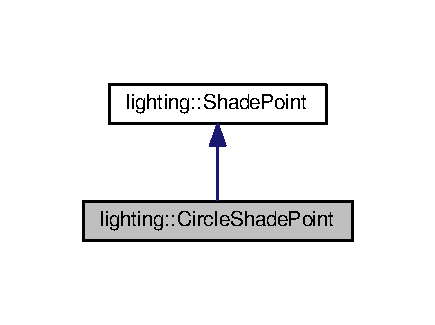
\includegraphics[width=209pt]{classlighting_1_1CircleShadePoint__inherit__graph}
\end{center}
\end{figure}


Collaboration diagram for lighting\+:\+:Circle\+Shade\+Point\+:\nopagebreak
\begin{figure}[H]
\begin{center}
\leavevmode
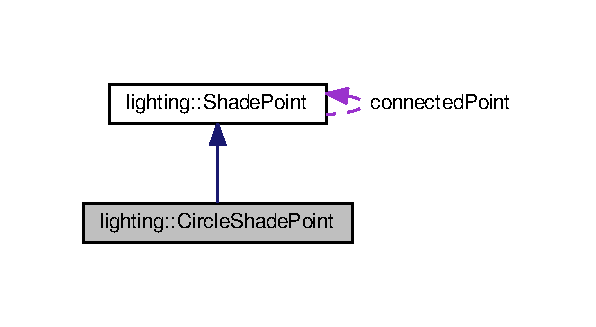
\includegraphics[width=286pt]{classlighting_1_1CircleShadePoint__coll__graph}
\end{center}
\end{figure}
\subsection*{Public Member Functions}
\begin{DoxyCompactItemize}
\item 
\hyperlink{classlighting_1_1CircleShadePoint_aef73e6c1a0e5ee8a099cbce37a7ab919}{Circle\+Shade\+Point} (float \hyperlink{classlighting_1_1ShadePoint_a087db3eacccf6731f674f123c22400ec}{x}, float \hyperlink{classlighting_1_1ShadePoint_a427350496a448f0dd7424955a6c21ea2}{y})
\begin{DoxyCompactList}\small\item\em Initializes a new instance of the \hyperlink{classlighting_1_1CircleShadePoint}{Circle\+Shade\+Point} class. \end{DoxyCompactList}\item 
\hyperlink{classlighting_1_1CircleShadePoint}{Circle\+Shade\+Point} $\ast$ \hyperlink{classlighting_1_1CircleShadePoint_aada35a7aca1f2aaecc9bf0e1ecc67ee1}{get\+Connect\+Point} ()
\begin{DoxyCompactList}\small\item\em Gets the other endpoint of the line. May be 
\begin{DoxyCode}
\textcolor{keyword}{nullptr}
\end{DoxyCode}
. \end{DoxyCompactList}\end{DoxyCompactItemize}
\subsection*{Public Attributes}
\begin{DoxyCompactItemize}
\item 
float \hyperlink{classlighting_1_1CircleShadePoint_a4b174fb379fd8d03ba4a5c47877b38ac}{rads}
\begin{DoxyCompactList}\small\item\em The angle of the coordinates when rotated around origin (0, 0). \end{DoxyCompactList}\item 
unsigned int \hyperlink{classlighting_1_1CircleShadePoint_a3a48629b0aebab194ab7d139d496c2da}{radix\+Val}
\begin{DoxyCompactList}\small\item\em The integer value represented \hyperlink{classlighting_1_1CircleShadePoint_a4b174fb379fd8d03ba4a5c47877b38ac}{rads} at a certain precision. \end{DoxyCompactList}\end{DoxyCompactItemize}
\subsection*{Additional Inherited Members}


\subsection{Constructor \& Destructor Documentation}
\index{lighting\+::\+Circle\+Shade\+Point@{lighting\+::\+Circle\+Shade\+Point}!Circle\+Shade\+Point@{Circle\+Shade\+Point}}
\index{Circle\+Shade\+Point@{Circle\+Shade\+Point}!lighting\+::\+Circle\+Shade\+Point@{lighting\+::\+Circle\+Shade\+Point}}
\subsubsection[{\texorpdfstring{Circle\+Shade\+Point(float x, float y)}{CircleShadePoint(float x, float y)}}]{\setlength{\rightskip}{0pt plus 5cm}lighting\+::\+Circle\+Shade\+Point\+::\+Circle\+Shade\+Point (
\begin{DoxyParamCaption}
\item[{float}]{x, }
\item[{float}]{y}
\end{DoxyParamCaption}
)}\hypertarget{classlighting_1_1CircleShadePoint_aef73e6c1a0e5ee8a099cbce37a7ab919}{}\label{classlighting_1_1CircleShadePoint_aef73e6c1a0e5ee8a099cbce37a7ab919}


Initializes a new instance of the \hyperlink{classlighting_1_1CircleShadePoint}{Circle\+Shade\+Point} class. 


\begin{DoxyParams}{Parameters}
{\em x} & The x.\\
\hline
{\em y} & The y.\\
\hline
\end{DoxyParams}


\subsection{Member Function Documentation}
\index{lighting\+::\+Circle\+Shade\+Point@{lighting\+::\+Circle\+Shade\+Point}!get\+Connect\+Point@{get\+Connect\+Point}}
\index{get\+Connect\+Point@{get\+Connect\+Point}!lighting\+::\+Circle\+Shade\+Point@{lighting\+::\+Circle\+Shade\+Point}}
\subsubsection[{\texorpdfstring{get\+Connect\+Point()}{getConnectPoint()}}]{\setlength{\rightskip}{0pt plus 5cm}{\bf Circle\+Shade\+Point}$\ast$ lighting\+::\+Circle\+Shade\+Point\+::get\+Connect\+Point (
\begin{DoxyParamCaption}
{}
\end{DoxyParamCaption}
)\hspace{0.3cm}{\ttfamily [inline]}}\hypertarget{classlighting_1_1CircleShadePoint_aada35a7aca1f2aaecc9bf0e1ecc67ee1}{}\label{classlighting_1_1CircleShadePoint_aada35a7aca1f2aaecc9bf0e1ecc67ee1}


Gets the other endpoint of the line. May be 
\begin{DoxyCode}
\textcolor{keyword}{nullptr}
\end{DoxyCode}
. 

\begin{DoxyReturn}{Returns}
The other endpoint, stored in the \hyperlink{classlighting_1_1ShadePoint_a0840495febcd385a90e89e003aa15972}{Shade\+Point\+::connected\+Point} attribute.
\end{DoxyReturn}


\subsection{Member Data Documentation}
\index{lighting\+::\+Circle\+Shade\+Point@{lighting\+::\+Circle\+Shade\+Point}!radix\+Val@{radix\+Val}}
\index{radix\+Val@{radix\+Val}!lighting\+::\+Circle\+Shade\+Point@{lighting\+::\+Circle\+Shade\+Point}}
\subsubsection[{\texorpdfstring{radix\+Val}{radixVal}}]{\setlength{\rightskip}{0pt plus 5cm}unsigned int lighting\+::\+Circle\+Shade\+Point\+::radix\+Val}\hypertarget{classlighting_1_1CircleShadePoint_a3a48629b0aebab194ab7d139d496c2da}{}\label{classlighting_1_1CircleShadePoint_a3a48629b0aebab194ab7d139d496c2da}


The integer value represented \hyperlink{classlighting_1_1CircleShadePoint_a4b174fb379fd8d03ba4a5c47877b38ac}{rads} at a certain precision. 

\index{lighting\+::\+Circle\+Shade\+Point@{lighting\+::\+Circle\+Shade\+Point}!rads@{rads}}
\index{rads@{rads}!lighting\+::\+Circle\+Shade\+Point@{lighting\+::\+Circle\+Shade\+Point}}
\subsubsection[{\texorpdfstring{rads}{rads}}]{\setlength{\rightskip}{0pt plus 5cm}float lighting\+::\+Circle\+Shade\+Point\+::rads}\hypertarget{classlighting_1_1CircleShadePoint_a4b174fb379fd8d03ba4a5c47877b38ac}{}\label{classlighting_1_1CircleShadePoint_a4b174fb379fd8d03ba4a5c47877b38ac}


The angle of the coordinates when rotated around origin (0, 0). 



The documentation for this class was generated from the following files\+:\begin{DoxyCompactItemize}
\item 
Circle\+Shade\+Point.\+h\item 
Circle\+Shade\+Point.\+cpp\end{DoxyCompactItemize}

\hypertarget{classlighting_1_1DirectionalLightSource}{}\section{lighting\+:\+:Directional\+Light\+Source Class Reference}
\label{classlighting_1_1DirectionalLightSource}\index{lighting\+::\+Directional\+Light\+Source@{lighting\+::\+Directional\+Light\+Source}}


Represents a light in the form of a flash light or any light beam limited to an angle  




{\ttfamily \#include $<$Directional\+Light\+Source.\+h$>$}



Inheritance diagram for lighting\+:\+:Directional\+Light\+Source\+:\nopagebreak
\begin{figure}[H]
\begin{center}
\leavevmode
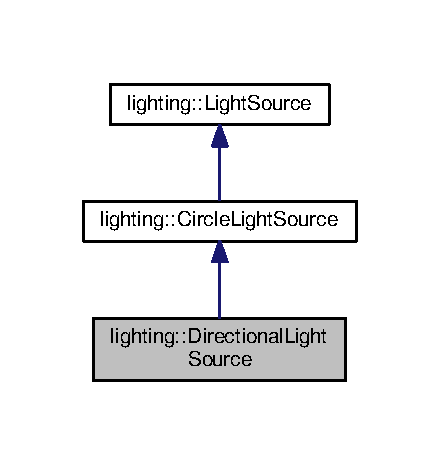
\includegraphics[width=211pt]{classlighting_1_1DirectionalLightSource__inherit__graph}
\end{center}
\end{figure}


Collaboration diagram for lighting\+:\+:Directional\+Light\+Source\+:\nopagebreak
\begin{figure}[H]
\begin{center}
\leavevmode
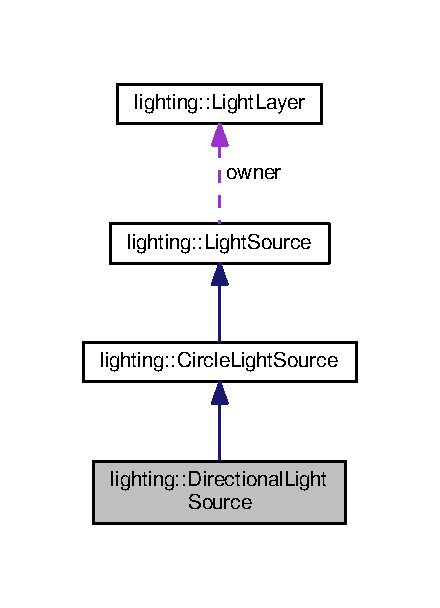
\includegraphics[width=211pt]{classlighting_1_1DirectionalLightSource__coll__graph}
\end{center}
\end{figure}
\subsection*{Public Member Functions}
\begin{DoxyCompactItemize}
\item 
\hyperlink{classlighting_1_1DirectionalLightSource_a65a9f9b9c9e624c4d9a2936dc86fa0b8}{Directional\+Light\+Source} (\hyperlink{classlighting_1_1LightLayer}{Light\+Layer} $\ast$owner\+Light\+Layer, int \hyperlink{classlighting_1_1CircleLightSource_a4da9b32f524563c2faeba5ea81dfe6fb}{radius}, float degs, uint8\+\_\+t r=U\+I\+N\+T8\+\_\+\+M\+AX, uint8\+\_\+t g=U\+I\+N\+T8\+\_\+\+M\+AX, uint8\+\_\+t b=U\+I\+N\+T8\+\_\+\+M\+AX)
\begin{DoxyCompactList}\small\item\em Initializes a new instance of the \hyperlink{classlighting_1_1DirectionalLightSource}{Directional\+Light\+Source} class. Initializes all of the bitmaps and sets their sizes. Adds itself to {\itshape owner\+Light\+Layer} . \end{DoxyCompactList}\item 
virtual void \hyperlink{classlighting_1_1DirectionalLightSource_a52f9f09a4088a44bf3f8b08df435a7aa}{draw\+Local} () override
\begin{DoxyCompactList}\small\item\em Draws the beam and shadows to the bitmap \hyperlink{classlighting_1_1DirectionalLightSource_afc3f2e73813a6d9c035aa0d58ad5d37c}{directional\+L\+Source\+Map}. \end{DoxyCompactList}\item 
virtual void \hyperlink{classlighting_1_1DirectionalLightSource_ab41be6321df178f861cd71462ab47553}{draw\+To\+Light\+Map} () override
\begin{DoxyCompactList}\small\item\em Draws light beam to the light\+Map. Assumes light\+Map is already set to target bitmap. \end{DoxyCompactList}\item 
void \hyperlink{classlighting_1_1DirectionalLightSource_a744ef9d945ccd0ea2dcfe94582c0515b}{set\+Degs} (float degs)
\begin{DoxyCompactList}\small\item\em Sets the angle of the beam in degrees. \end{DoxyCompactList}\item 
void \hyperlink{classlighting_1_1DirectionalLightSource_ada5610905c7449a464eb89496b026b55}{change\+Degs} (float delta\+Degs)
\begin{DoxyCompactList}\small\item\em Changes the angle of the beam. \end{DoxyCompactList}\item 
void \hyperlink{classlighting_1_1DirectionalLightSource_a0d2f2c2dc0899e45540474391960ccd0}{set\+Rads} (float \hyperlink{classlighting_1_1DirectionalLightSource_af31141ab246928972aa52224e17ae46c}{rads})
\begin{DoxyCompactList}\small\item\em Sets the angle of the beam. \end{DoxyCompactList}\item 
void \hyperlink{classlighting_1_1DirectionalLightSource_a8737004541be45ccf76a77d52ea5ad0e}{change\+Rads} (float delta\+Rads)
\begin{DoxyCompactList}\small\item\em Changes the angle of the beam. \end{DoxyCompactList}\end{DoxyCompactItemize}
\subsection*{Protected Attributes}
\begin{DoxyCompactItemize}
\item 
A\+L\+L\+E\+G\+R\+O\+\_\+\+B\+I\+T\+M\+AP $\ast$ \hyperlink{classlighting_1_1DirectionalLightSource_a021658da101e47c909858b2c17d387ff}{directional\+L\+Source\+Map\+Save}
\begin{DoxyCompactList}\small\item\em Bitmap of the directional light, created in constructor and is not changed \end{DoxyCompactList}\item 
A\+L\+L\+E\+G\+R\+O\+\_\+\+B\+I\+T\+M\+AP $\ast$ \hyperlink{classlighting_1_1DirectionalLightSource_afc3f2e73813a6d9c035aa0d58ad5d37c}{directional\+L\+Source\+Map}
\begin{DoxyCompactList}\small\item\em Bitmap where \hyperlink{classlighting_1_1CircleLightSource_a382414c9318853e93c85bc64bcd19f4e}{Circle\+Light\+Source\+::shade\+Map} and \hyperlink{classlighting_1_1DirectionalLightSource_a021658da101e47c909858b2c17d387ff}{directional\+L\+Source\+Map\+Save} are combined. \end{DoxyCompactList}\item 
int \hyperlink{classlighting_1_1DirectionalLightSource_af4372a31b5f7938c18723f53265922e7}{directional\+L\+SourceW}
\begin{DoxyCompactList}\small\item\em The width of the directional\+L\+Source bitmaps. \end{DoxyCompactList}\item 
int \hyperlink{classlighting_1_1DirectionalLightSource_a6587335669534fd8f4727c73dbd49c28}{directional\+L\+SourceH}
\begin{DoxyCompactList}\small\item\em The height of the directional\+L\+Source bitmaps. \end{DoxyCompactList}\item 
float \hyperlink{classlighting_1_1DirectionalLightSource_af31141ab246928972aa52224e17ae46c}{rads}
\begin{DoxyCompactList}\small\item\em The angle of the beam (not the spread of it, in radians) \end{DoxyCompactList}\end{DoxyCompactItemize}
\subsection*{Additional Inherited Members}


\subsection{Detailed Description}
Represents a light in the form of a flash light or any light beam limited to an angle 

\begin{DoxySeeAlso}{See also}
\hyperlink{classlighting_1_1CircleLightSource}{Circle\+Light\+Source}


\end{DoxySeeAlso}


\subsection{Constructor \& Destructor Documentation}
\index{lighting\+::\+Directional\+Light\+Source@{lighting\+::\+Directional\+Light\+Source}!Directional\+Light\+Source@{Directional\+Light\+Source}}
\index{Directional\+Light\+Source@{Directional\+Light\+Source}!lighting\+::\+Directional\+Light\+Source@{lighting\+::\+Directional\+Light\+Source}}
\subsubsection[{\texorpdfstring{Directional\+Light\+Source(\+Light\+Layer $\ast$owner\+Light\+Layer, int radius, float degs, uint8\+\_\+t r=\+U\+I\+N\+T8\+\_\+\+M\+A\+X, uint8\+\_\+t g=\+U\+I\+N\+T8\+\_\+\+M\+A\+X, uint8\+\_\+t b=\+U\+I\+N\+T8\+\_\+\+M\+A\+X)}{DirectionalLightSource(LightLayer *ownerLightLayer, int radius, float degs, uint8_t r=UINT8_MAX, uint8_t g=UINT8_MAX, uint8_t b=UINT8_MAX)}}]{\setlength{\rightskip}{0pt plus 5cm}lighting\+::\+Directional\+Light\+Source\+::\+Directional\+Light\+Source (
\begin{DoxyParamCaption}
\item[{{\bf Light\+Layer} $\ast$}]{owner\+Light\+Layer, }
\item[{int}]{radius, }
\item[{float}]{degs, }
\item[{uint8\+\_\+t}]{r = {\ttfamily UINT8\+\_\+MAX}, }
\item[{uint8\+\_\+t}]{g = {\ttfamily UINT8\+\_\+MAX}, }
\item[{uint8\+\_\+t}]{b = {\ttfamily UINT8\+\_\+MAX}}
\end{DoxyParamCaption}
)}\hypertarget{classlighting_1_1DirectionalLightSource_a65a9f9b9c9e624c4d9a2936dc86fa0b8}{}\label{classlighting_1_1DirectionalLightSource_a65a9f9b9c9e624c4d9a2936dc86fa0b8}


Initializes a new instance of the \hyperlink{classlighting_1_1DirectionalLightSource}{Directional\+Light\+Source} class. Initializes all of the bitmaps and sets their sizes. Adds itself to {\itshape owner\+Light\+Layer} . 


\begin{DoxyParams}{Parameters}
{\em owner\+Light\+Layer} & The light\+Layer that owns it.\\
\hline
{\em radius} & The radius of the light.\\
\hline
{\em degs} & The spread of the light beam.\\
\hline
{\em r} & The red color value for the light.\\
\hline
{\em g} & The green color value for the light.\\
\hline
{\em b} & The blue color value for the light.\\
\hline
\end{DoxyParams}


\subsection{Member Function Documentation}
\index{lighting\+::\+Directional\+Light\+Source@{lighting\+::\+Directional\+Light\+Source}!change\+Degs@{change\+Degs}}
\index{change\+Degs@{change\+Degs}!lighting\+::\+Directional\+Light\+Source@{lighting\+::\+Directional\+Light\+Source}}
\subsubsection[{\texorpdfstring{change\+Degs(float delta\+Degs)}{changeDegs(float deltaDegs)}}]{\setlength{\rightskip}{0pt plus 5cm}void lighting\+::\+Directional\+Light\+Source\+::change\+Degs (
\begin{DoxyParamCaption}
\item[{float}]{delta\+Degs}
\end{DoxyParamCaption}
)\hspace{0.3cm}{\ttfamily [inline]}}\hypertarget{classlighting_1_1DirectionalLightSource_ada5610905c7449a464eb89496b026b55}{}\label{classlighting_1_1DirectionalLightSource_ada5610905c7449a464eb89496b026b55}


Changes the angle of the beam. 


\begin{DoxyParams}{Parameters}
{\em delta\+Degs} & The change in degrees.\\
\hline
\end{DoxyParams}
\index{lighting\+::\+Directional\+Light\+Source@{lighting\+::\+Directional\+Light\+Source}!change\+Rads@{change\+Rads}}
\index{change\+Rads@{change\+Rads}!lighting\+::\+Directional\+Light\+Source@{lighting\+::\+Directional\+Light\+Source}}
\subsubsection[{\texorpdfstring{change\+Rads(float delta\+Rads)}{changeRads(float deltaRads)}}]{\setlength{\rightskip}{0pt plus 5cm}void lighting\+::\+Directional\+Light\+Source\+::change\+Rads (
\begin{DoxyParamCaption}
\item[{float}]{delta\+Rads}
\end{DoxyParamCaption}
)\hspace{0.3cm}{\ttfamily [inline]}}\hypertarget{classlighting_1_1DirectionalLightSource_a8737004541be45ccf76a77d52ea5ad0e}{}\label{classlighting_1_1DirectionalLightSource_a8737004541be45ccf76a77d52ea5ad0e}


Changes the angle of the beam. 


\begin{DoxyParams}{Parameters}
{\em delta\+Rads} & The change in rads.\\
\hline
\end{DoxyParams}
\index{lighting\+::\+Directional\+Light\+Source@{lighting\+::\+Directional\+Light\+Source}!draw\+Local@{draw\+Local}}
\index{draw\+Local@{draw\+Local}!lighting\+::\+Directional\+Light\+Source@{lighting\+::\+Directional\+Light\+Source}}
\subsubsection[{\texorpdfstring{draw\+Local() override}{drawLocal() override}}]{\setlength{\rightskip}{0pt plus 5cm}void lighting\+::\+Directional\+Light\+Source\+::draw\+Local (
\begin{DoxyParamCaption}
{}
\end{DoxyParamCaption}
)\hspace{0.3cm}{\ttfamily [override]}, {\ttfamily [virtual]}}\hypertarget{classlighting_1_1DirectionalLightSource_a52f9f09a4088a44bf3f8b08df435a7aa}{}\label{classlighting_1_1DirectionalLightSource_a52f9f09a4088a44bf3f8b08df435a7aa}


Draws the beam and shadows to the bitmap \hyperlink{classlighting_1_1DirectionalLightSource_afc3f2e73813a6d9c035aa0d58ad5d37c}{directional\+L\+Source\+Map}. 



Reimplemented from \hyperlink{classlighting_1_1CircleLightSource_a6ab6f8f8eaf003e52ac2c86d88496c77}{lighting\+::\+Circle\+Light\+Source}.

\index{lighting\+::\+Directional\+Light\+Source@{lighting\+::\+Directional\+Light\+Source}!draw\+To\+Light\+Map@{draw\+To\+Light\+Map}}
\index{draw\+To\+Light\+Map@{draw\+To\+Light\+Map}!lighting\+::\+Directional\+Light\+Source@{lighting\+::\+Directional\+Light\+Source}}
\subsubsection[{\texorpdfstring{draw\+To\+Light\+Map() override}{drawToLightMap() override}}]{\setlength{\rightskip}{0pt plus 5cm}void lighting\+::\+Directional\+Light\+Source\+::draw\+To\+Light\+Map (
\begin{DoxyParamCaption}
{}
\end{DoxyParamCaption}
)\hspace{0.3cm}{\ttfamily [override]}, {\ttfamily [virtual]}}\hypertarget{classlighting_1_1DirectionalLightSource_ab41be6321df178f861cd71462ab47553}{}\label{classlighting_1_1DirectionalLightSource_ab41be6321df178f861cd71462ab47553}


Draws light beam to the light\+Map. Assumes light\+Map is already set to target bitmap. 



Reimplemented from \hyperlink{classlighting_1_1CircleLightSource_ab0f9107c09ae9c6966bab14538505894}{lighting\+::\+Circle\+Light\+Source}.

\index{lighting\+::\+Directional\+Light\+Source@{lighting\+::\+Directional\+Light\+Source}!set\+Degs@{set\+Degs}}
\index{set\+Degs@{set\+Degs}!lighting\+::\+Directional\+Light\+Source@{lighting\+::\+Directional\+Light\+Source}}
\subsubsection[{\texorpdfstring{set\+Degs(float degs)}{setDegs(float degs)}}]{\setlength{\rightskip}{0pt plus 5cm}void lighting\+::\+Directional\+Light\+Source\+::set\+Degs (
\begin{DoxyParamCaption}
\item[{float}]{degs}
\end{DoxyParamCaption}
)\hspace{0.3cm}{\ttfamily [inline]}}\hypertarget{classlighting_1_1DirectionalLightSource_a744ef9d945ccd0ea2dcfe94582c0515b}{}\label{classlighting_1_1DirectionalLightSource_a744ef9d945ccd0ea2dcfe94582c0515b}


Sets the angle of the beam in degrees. 


\begin{DoxyParams}{Parameters}
{\em degs} & The angle of the beam.\\
\hline
\end{DoxyParams}
\index{lighting\+::\+Directional\+Light\+Source@{lighting\+::\+Directional\+Light\+Source}!set\+Rads@{set\+Rads}}
\index{set\+Rads@{set\+Rads}!lighting\+::\+Directional\+Light\+Source@{lighting\+::\+Directional\+Light\+Source}}
\subsubsection[{\texorpdfstring{set\+Rads(float rads)}{setRads(float rads)}}]{\setlength{\rightskip}{0pt plus 5cm}void lighting\+::\+Directional\+Light\+Source\+::set\+Rads (
\begin{DoxyParamCaption}
\item[{float}]{rads}
\end{DoxyParamCaption}
)\hspace{0.3cm}{\ttfamily [inline]}}\hypertarget{classlighting_1_1DirectionalLightSource_a0d2f2c2dc0899e45540474391960ccd0}{}\label{classlighting_1_1DirectionalLightSource_a0d2f2c2dc0899e45540474391960ccd0}


Sets the angle of the beam. 


\begin{DoxyParams}{Parameters}
{\em rads} & The angle to set the beam to.\\
\hline
\end{DoxyParams}


\subsection{Member Data Documentation}
\index{lighting\+::\+Directional\+Light\+Source@{lighting\+::\+Directional\+Light\+Source}!directional\+L\+SourceH@{directional\+L\+SourceH}}
\index{directional\+L\+SourceH@{directional\+L\+SourceH}!lighting\+::\+Directional\+Light\+Source@{lighting\+::\+Directional\+Light\+Source}}
\subsubsection[{\texorpdfstring{directional\+L\+SourceH}{directionalLSourceH}}]{\setlength{\rightskip}{0pt plus 5cm}int lighting\+::\+Directional\+Light\+Source\+::directional\+L\+SourceH\hspace{0.3cm}{\ttfamily [protected]}}\hypertarget{classlighting_1_1DirectionalLightSource_a6587335669534fd8f4727c73dbd49c28}{}\label{classlighting_1_1DirectionalLightSource_a6587335669534fd8f4727c73dbd49c28}


The height of the directional\+L\+Source bitmaps. 

\index{lighting\+::\+Directional\+Light\+Source@{lighting\+::\+Directional\+Light\+Source}!directional\+L\+Source\+Map@{directional\+L\+Source\+Map}}
\index{directional\+L\+Source\+Map@{directional\+L\+Source\+Map}!lighting\+::\+Directional\+Light\+Source@{lighting\+::\+Directional\+Light\+Source}}
\subsubsection[{\texorpdfstring{directional\+L\+Source\+Map}{directionalLSourceMap}}]{\setlength{\rightskip}{0pt plus 5cm}A\+L\+L\+E\+G\+R\+O\+\_\+\+B\+I\+T\+M\+AP$\ast$ lighting\+::\+Directional\+Light\+Source\+::directional\+L\+Source\+Map\hspace{0.3cm}{\ttfamily [protected]}}\hypertarget{classlighting_1_1DirectionalLightSource_afc3f2e73813a6d9c035aa0d58ad5d37c}{}\label{classlighting_1_1DirectionalLightSource_afc3f2e73813a6d9c035aa0d58ad5d37c}


Bitmap where \hyperlink{classlighting_1_1CircleLightSource_a382414c9318853e93c85bc64bcd19f4e}{Circle\+Light\+Source\+::shade\+Map} and \hyperlink{classlighting_1_1DirectionalLightSource_a021658da101e47c909858b2c17d387ff}{directional\+L\+Source\+Map\+Save} are combined. 

\index{lighting\+::\+Directional\+Light\+Source@{lighting\+::\+Directional\+Light\+Source}!directional\+L\+Source\+Map\+Save@{directional\+L\+Source\+Map\+Save}}
\index{directional\+L\+Source\+Map\+Save@{directional\+L\+Source\+Map\+Save}!lighting\+::\+Directional\+Light\+Source@{lighting\+::\+Directional\+Light\+Source}}
\subsubsection[{\texorpdfstring{directional\+L\+Source\+Map\+Save}{directionalLSourceMapSave}}]{\setlength{\rightskip}{0pt plus 5cm}A\+L\+L\+E\+G\+R\+O\+\_\+\+B\+I\+T\+M\+AP$\ast$ lighting\+::\+Directional\+Light\+Source\+::directional\+L\+Source\+Map\+Save\hspace{0.3cm}{\ttfamily [protected]}}\hypertarget{classlighting_1_1DirectionalLightSource_a021658da101e47c909858b2c17d387ff}{}\label{classlighting_1_1DirectionalLightSource_a021658da101e47c909858b2c17d387ff}


Bitmap of the directional light, created in constructor and is not changed 

\index{lighting\+::\+Directional\+Light\+Source@{lighting\+::\+Directional\+Light\+Source}!directional\+L\+SourceW@{directional\+L\+SourceW}}
\index{directional\+L\+SourceW@{directional\+L\+SourceW}!lighting\+::\+Directional\+Light\+Source@{lighting\+::\+Directional\+Light\+Source}}
\subsubsection[{\texorpdfstring{directional\+L\+SourceW}{directionalLSourceW}}]{\setlength{\rightskip}{0pt plus 5cm}int lighting\+::\+Directional\+Light\+Source\+::directional\+L\+SourceW\hspace{0.3cm}{\ttfamily [protected]}}\hypertarget{classlighting_1_1DirectionalLightSource_af4372a31b5f7938c18723f53265922e7}{}\label{classlighting_1_1DirectionalLightSource_af4372a31b5f7938c18723f53265922e7}


The width of the directional\+L\+Source bitmaps. 

\index{lighting\+::\+Directional\+Light\+Source@{lighting\+::\+Directional\+Light\+Source}!rads@{rads}}
\index{rads@{rads}!lighting\+::\+Directional\+Light\+Source@{lighting\+::\+Directional\+Light\+Source}}
\subsubsection[{\texorpdfstring{rads}{rads}}]{\setlength{\rightskip}{0pt plus 5cm}float lighting\+::\+Directional\+Light\+Source\+::rads\hspace{0.3cm}{\ttfamily [protected]}}\hypertarget{classlighting_1_1DirectionalLightSource_af31141ab246928972aa52224e17ae46c}{}\label{classlighting_1_1DirectionalLightSource_af31141ab246928972aa52224e17ae46c}


The angle of the beam (not the spread of it, in radians) 



The documentation for this class was generated from the following files\+:\begin{DoxyCompactItemize}
\item 
Directional\+Light\+Source.\+h\item 
Directional\+Light\+Source.\+cpp\end{DoxyCompactItemize}

\hypertarget{classlighting_1_1GaussianBlurrer}{}\section{lighting\+:\+:Gaussian\+Blurrer Class Reference}
\label{classlighting_1_1GaussianBlurrer}\index{lighting\+::\+Gaussian\+Blurrer@{lighting\+::\+Gaussian\+Blurrer}}


Takes bitmaps and uses a two pass gaussian blur on it. Specify which shaders to use and the kernel\+Data. Adds itself to {\itshape owner} .  




{\ttfamily \#include $<$Gaussian\+Blurrer.\+h$>$}



Collaboration diagram for lighting\+:\+:Gaussian\+Blurrer\+:\nopagebreak
\begin{figure}[H]
\begin{center}
\leavevmode
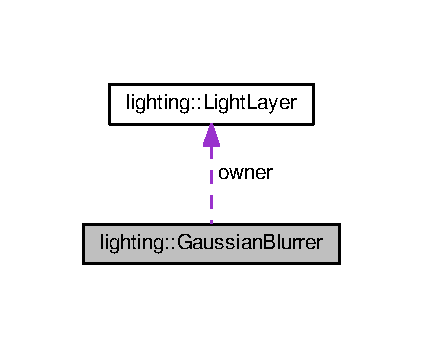
\includegraphics[width=203pt]{classlighting_1_1GaussianBlurrer__coll__graph}
\end{center}
\end{figure}
\subsection*{Public Member Functions}
\begin{DoxyCompactItemize}
\item 
\hyperlink{classlighting_1_1GaussianBlurrer_ad6586426f68f4e7527261951fe39f995}{Gaussian\+Blurrer} (\hyperlink{classlighting_1_1LightLayer}{Light\+Layer} $\ast$\hyperlink{classlighting_1_1GaussianBlurrer_ae673db1b5f734d90a45628a33cc73bd1}{owner}, \hyperlink{classlighting_1_1GaussianKernelData}{Gaussian\+Kernel\+Data} \&kernel\+Data, const std\+::string \&vert\+Shader\+Path, const std\+::string \&pixel\+Shader\+PathX, const std\+::string \&pixel\+Shader\+PathY, A\+L\+L\+E\+G\+R\+O\+\_\+\+S\+H\+A\+D\+E\+R\+\_\+\+P\+L\+A\+T\+F\+O\+RM platform=A\+L\+L\+E\+G\+R\+O\+\_\+\+S\+H\+A\+D\+E\+R\+\_\+\+A\+U\+TO)
\begin{DoxyCompactList}\small\item\em Initializes a new instance of the \hyperlink{classlighting_1_1GaussianBlurrer}{Gaussian\+Blurrer} class. Creating new shaders with the proper {\itshape kernel\+Data} . \end{DoxyCompactList}\item 
void \hyperlink{classlighting_1_1GaussianBlurrer_a8422fd11341d886f0951552bdc038f5b}{blur} (A\+L\+L\+E\+G\+R\+O\+\_\+\+B\+I\+T\+M\+AP $\ast$map\+To\+Blur, A\+L\+L\+E\+G\+R\+O\+\_\+\+B\+I\+T\+M\+AP $\ast$placeholder)
\begin{DoxyCompactList}\small\item\em Called by Light\+Map. The {\itshape map\+To\+Blur}  will be fully gaussian blurred and the placeholder bitmap will be horizontally blurred. (W\+A\+R\+N\+I\+NG S\+H\+A\+D\+ER N\+OT S\+ET TO N\+U\+L\+L\+P\+TR W\+H\+EN F\+I\+N\+I\+S\+H\+ED). \end{DoxyCompactList}\item 
\hyperlink{classlighting_1_1GaussianBlurrer_ae3b3470c59d86f3837b639961f41cb13}{$\sim$\+Gaussian\+Blurrer} ()
\begin{DoxyCompactList}\small\item\em Finalizes an instance of the \hyperlink{classlighting_1_1GaussianBlurrer}{Gaussian\+Blurrer} class. Removes itself from {\itshape owner} . \end{DoxyCompactList}\end{DoxyCompactItemize}
\subsection*{Protected Member Functions}
\begin{DoxyCompactItemize}
\item 
A\+L\+L\+E\+G\+R\+O\+\_\+\+S\+H\+A\+D\+ER $\ast$ \hyperlink{classlighting_1_1GaussianBlurrer_a6c13e999dd54c2dbbbfb6af5ab800412}{get\+Shader} (const std\+::string \&vert\+Shader\+Path, const std\+::string \&pixel\+Shader\+Path, A\+L\+L\+E\+G\+R\+O\+\_\+\+S\+H\+A\+D\+E\+R\+\_\+\+P\+L\+A\+T\+F\+O\+RM platform)
\begin{DoxyCompactList}\small\item\em Creates a new shader using the paths specified. \end{DoxyCompactList}\end{DoxyCompactItemize}
\subsection*{Protected Attributes}
\begin{DoxyCompactItemize}
\item 
A\+L\+L\+E\+G\+R\+O\+\_\+\+S\+H\+A\+D\+ER $\ast$ \hyperlink{classlighting_1_1GaussianBlurrer_a36d10a62e2fd99e1182c596425fbacfa}{shaderX}
\begin{DoxyCompactList}\small\item\em The horizontal gaussian shader (called first). \end{DoxyCompactList}\item 
A\+L\+L\+E\+G\+R\+O\+\_\+\+S\+H\+A\+D\+ER $\ast$ \hyperlink{classlighting_1_1GaussianBlurrer_a57c41b5a1dd0712e98d085a8a90172d4}{shaderY}
\begin{DoxyCompactList}\small\item\em The vertial gaussian shader (called last). \end{DoxyCompactList}\item 
\hyperlink{classlighting_1_1LightLayer}{Light\+Layer} $\ast$ \hyperlink{classlighting_1_1GaussianBlurrer_ae673db1b5f734d90a45628a33cc73bd1}{owner}
\begin{DoxyCompactList}\small\item\em The \hyperlink{classlighting_1_1LightLayer}{Light\+Layer} that owns 
\begin{DoxyCode}
\textcolor{keyword}{this}
\end{DoxyCode}
. \end{DoxyCompactList}\end{DoxyCompactItemize}


\subsection{Detailed Description}
Takes bitmaps and uses a two pass gaussian blur on it. Specify which shaders to use and the kernel\+Data. Adds itself to {\itshape owner} . 



\subsection{Constructor \& Destructor Documentation}
\index{lighting\+::\+Gaussian\+Blurrer@{lighting\+::\+Gaussian\+Blurrer}!Gaussian\+Blurrer@{Gaussian\+Blurrer}}
\index{Gaussian\+Blurrer@{Gaussian\+Blurrer}!lighting\+::\+Gaussian\+Blurrer@{lighting\+::\+Gaussian\+Blurrer}}
\subsubsection[{\texorpdfstring{Gaussian\+Blurrer(\+Light\+Layer $\ast$owner, Gaussian\+Kernel\+Data \&kernel\+Data, const std\+::string \&vert\+Shader\+Path, const std\+::string \&pixel\+Shader\+Path\+X, const std\+::string \&pixel\+Shader\+Path\+Y, A\+L\+L\+E\+G\+R\+O\+\_\+\+S\+H\+A\+D\+E\+R\+\_\+\+P\+L\+A\+T\+F\+O\+R\+M platform=\+A\+L\+L\+E\+G\+R\+O\+\_\+\+S\+H\+A\+D\+E\+R\+\_\+\+A\+U\+T\+O)}{GaussianBlurrer(LightLayer *owner, GaussianKernelData &kernelData, const std::string &vertShaderPath, const std::string &pixelShaderPathX, const std::string &pixelShaderPathY, ALLEGRO_SHADER_PLATFORM platform=ALLEGRO_SHADER_AUTO)}}]{\setlength{\rightskip}{0pt plus 5cm}lighting\+::\+Gaussian\+Blurrer\+::\+Gaussian\+Blurrer (
\begin{DoxyParamCaption}
\item[{{\bf Light\+Layer} $\ast$}]{owner, }
\item[{{\bf Gaussian\+Kernel\+Data} \&}]{kernel\+Data, }
\item[{const std\+::string \&}]{vert\+Shader\+Path, }
\item[{const std\+::string \&}]{pixel\+Shader\+PathX, }
\item[{const std\+::string \&}]{pixel\+Shader\+PathY, }
\item[{A\+L\+L\+E\+G\+R\+O\+\_\+\+S\+H\+A\+D\+E\+R\+\_\+\+P\+L\+A\+T\+F\+O\+RM}]{platform = {\ttfamily ALLEGRO\+\_\+SHADER\+\_\+AUTO}}
\end{DoxyParamCaption}
)}\hypertarget{classlighting_1_1GaussianBlurrer_ad6586426f68f4e7527261951fe39f995}{}\label{classlighting_1_1GaussianBlurrer_ad6586426f68f4e7527261951fe39f995}


Initializes a new instance of the \hyperlink{classlighting_1_1GaussianBlurrer}{Gaussian\+Blurrer} class. Creating new shaders with the proper {\itshape kernel\+Data} . 


\begin{DoxyParams}{Parameters}
{\em owner} & The \hyperlink{classlighting_1_1LightLayer}{Light\+Layer} that owns 
\begin{DoxyCode}
\textcolor{keyword}{this}
\end{DoxyCode}
.\\
\hline
{\em kernel\+Data} & The \hyperlink{classlighting_1_1GaussianKernelData}{Gaussian\+Kernel\+Data} used to set the variables of the shaders. Uses the Pixel\+Offsets and Pixel\+Weights to set the shaders. The size of Pixel\+Offsets and Pixel\+Weights must be less than 12 (When generating the Kernel\+Data, use values less than 44)\\
\hline
{\em vert\+Shader\+Path} & The vertex shader path, must be compatible with Allegro (See their default shader for an example).\\
\hline
{\em pixel\+Shader\+PathX} & The pixel shader path for horizontal gaussian blur. Should have Bmp\+Width, Pixel\+Offsets, and Pixel\+Weights variables to set.\\
\hline
{\em pixel\+Shader\+PathY} & The pixel shader path for vertical gaussian blur. Should have Bmp\+Height, Pixel\+Offsets, and Pixel\+Weights variables to set.\\
\hline
{\em platform} & The platform to create the shaders on, H\+L\+SL or G\+L\+SL.\\
\hline
\end{DoxyParams}
\index{lighting\+::\+Gaussian\+Blurrer@{lighting\+::\+Gaussian\+Blurrer}!````~Gaussian\+Blurrer@{$\sim$\+Gaussian\+Blurrer}}
\index{````~Gaussian\+Blurrer@{$\sim$\+Gaussian\+Blurrer}!lighting\+::\+Gaussian\+Blurrer@{lighting\+::\+Gaussian\+Blurrer}}
\subsubsection[{\texorpdfstring{$\sim$\+Gaussian\+Blurrer()}{~GaussianBlurrer()}}]{\setlength{\rightskip}{0pt plus 5cm}lighting\+::\+Gaussian\+Blurrer\+::$\sim$\+Gaussian\+Blurrer (
\begin{DoxyParamCaption}
{}
\end{DoxyParamCaption}
)}\hypertarget{classlighting_1_1GaussianBlurrer_ae3b3470c59d86f3837b639961f41cb13}{}\label{classlighting_1_1GaussianBlurrer_ae3b3470c59d86f3837b639961f41cb13}


Finalizes an instance of the \hyperlink{classlighting_1_1GaussianBlurrer}{Gaussian\+Blurrer} class. Removes itself from {\itshape owner} . 



\subsection{Member Function Documentation}
\index{lighting\+::\+Gaussian\+Blurrer@{lighting\+::\+Gaussian\+Blurrer}!blur@{blur}}
\index{blur@{blur}!lighting\+::\+Gaussian\+Blurrer@{lighting\+::\+Gaussian\+Blurrer}}
\subsubsection[{\texorpdfstring{blur(\+A\+L\+L\+E\+G\+R\+O\+\_\+\+B\+I\+T\+M\+A\+P $\ast$map\+To\+Blur, A\+L\+L\+E\+G\+R\+O\+\_\+\+B\+I\+T\+M\+A\+P $\ast$placeholder)}{blur(ALLEGRO_BITMAP *mapToBlur, ALLEGRO_BITMAP *placeholder)}}]{\setlength{\rightskip}{0pt plus 5cm}void lighting\+::\+Gaussian\+Blurrer\+::blur (
\begin{DoxyParamCaption}
\item[{A\+L\+L\+E\+G\+R\+O\+\_\+\+B\+I\+T\+M\+AP $\ast$}]{map\+To\+Blur, }
\item[{A\+L\+L\+E\+G\+R\+O\+\_\+\+B\+I\+T\+M\+AP $\ast$}]{placeholder}
\end{DoxyParamCaption}
)}\hypertarget{classlighting_1_1GaussianBlurrer_a8422fd11341d886f0951552bdc038f5b}{}\label{classlighting_1_1GaussianBlurrer_a8422fd11341d886f0951552bdc038f5b}


Called by Light\+Map. The {\itshape map\+To\+Blur}  will be fully gaussian blurred and the placeholder bitmap will be horizontally blurred. (W\+A\+R\+N\+I\+NG S\+H\+A\+D\+ER N\+OT S\+ET TO N\+U\+L\+L\+P\+TR W\+H\+EN F\+I\+N\+I\+S\+H\+ED). 


\begin{DoxyParams}{Parameters}
{\em map\+To\+Blur} & The map to blur.\\
\hline
{\em placeholder} & The placeholder.\\
\hline
\end{DoxyParams}
\index{lighting\+::\+Gaussian\+Blurrer@{lighting\+::\+Gaussian\+Blurrer}!get\+Shader@{get\+Shader}}
\index{get\+Shader@{get\+Shader}!lighting\+::\+Gaussian\+Blurrer@{lighting\+::\+Gaussian\+Blurrer}}
\subsubsection[{\texorpdfstring{get\+Shader(const std\+::string \&vert\+Shader\+Path, const std\+::string \&pixel\+Shader\+Path, A\+L\+L\+E\+G\+R\+O\+\_\+\+S\+H\+A\+D\+E\+R\+\_\+\+P\+L\+A\+T\+F\+O\+R\+M platform)}{getShader(const std::string &vertShaderPath, const std::string &pixelShaderPath, ALLEGRO_SHADER_PLATFORM platform)}}]{\setlength{\rightskip}{0pt plus 5cm}A\+L\+L\+E\+G\+R\+O\+\_\+\+S\+H\+A\+D\+ER $\ast$ lighting\+::\+Gaussian\+Blurrer\+::get\+Shader (
\begin{DoxyParamCaption}
\item[{const std\+::string \&}]{vert\+Shader\+Path, }
\item[{const std\+::string \&}]{pixel\+Shader\+Path, }
\item[{A\+L\+L\+E\+G\+R\+O\+\_\+\+S\+H\+A\+D\+E\+R\+\_\+\+P\+L\+A\+T\+F\+O\+RM}]{platform}
\end{DoxyParamCaption}
)\hspace{0.3cm}{\ttfamily [protected]}}\hypertarget{classlighting_1_1GaussianBlurrer_a6c13e999dd54c2dbbbfb6af5ab800412}{}\label{classlighting_1_1GaussianBlurrer_a6c13e999dd54c2dbbbfb6af5ab800412}


Creates a new shader using the paths specified. 


\begin{DoxyParams}{Parameters}
{\em vert\+Shader\+Path} & The vertex shader path, must be compatible with Allegro (See their default shader for an example).\\
\hline
{\em pixel\+Shader\+Path} & The pixel shader path.\\
\hline
{\em platform} & The shader platform (H\+L\+SL or G\+L\+SL).\\
\hline
\end{DoxyParams}
\begin{DoxyReturn}{Returns}

\end{DoxyReturn}


\subsection{Member Data Documentation}
\index{lighting\+::\+Gaussian\+Blurrer@{lighting\+::\+Gaussian\+Blurrer}!owner@{owner}}
\index{owner@{owner}!lighting\+::\+Gaussian\+Blurrer@{lighting\+::\+Gaussian\+Blurrer}}
\subsubsection[{\texorpdfstring{owner}{owner}}]{\setlength{\rightskip}{0pt plus 5cm}{\bf Light\+Layer}$\ast$ lighting\+::\+Gaussian\+Blurrer\+::owner\hspace{0.3cm}{\ttfamily [protected]}}\hypertarget{classlighting_1_1GaussianBlurrer_ae673db1b5f734d90a45628a33cc73bd1}{}\label{classlighting_1_1GaussianBlurrer_ae673db1b5f734d90a45628a33cc73bd1}


The \hyperlink{classlighting_1_1LightLayer}{Light\+Layer} that owns 
\begin{DoxyCode}
\textcolor{keyword}{this}
\end{DoxyCode}
. 

\index{lighting\+::\+Gaussian\+Blurrer@{lighting\+::\+Gaussian\+Blurrer}!shaderX@{shaderX}}
\index{shaderX@{shaderX}!lighting\+::\+Gaussian\+Blurrer@{lighting\+::\+Gaussian\+Blurrer}}
\subsubsection[{\texorpdfstring{shaderX}{shaderX}}]{\setlength{\rightskip}{0pt plus 5cm}A\+L\+L\+E\+G\+R\+O\+\_\+\+S\+H\+A\+D\+ER$\ast$ lighting\+::\+Gaussian\+Blurrer\+::shaderX\hspace{0.3cm}{\ttfamily [protected]}}\hypertarget{classlighting_1_1GaussianBlurrer_a36d10a62e2fd99e1182c596425fbacfa}{}\label{classlighting_1_1GaussianBlurrer_a36d10a62e2fd99e1182c596425fbacfa}


The horizontal gaussian shader (called first). 

\index{lighting\+::\+Gaussian\+Blurrer@{lighting\+::\+Gaussian\+Blurrer}!shaderY@{shaderY}}
\index{shaderY@{shaderY}!lighting\+::\+Gaussian\+Blurrer@{lighting\+::\+Gaussian\+Blurrer}}
\subsubsection[{\texorpdfstring{shaderY}{shaderY}}]{\setlength{\rightskip}{0pt plus 5cm}A\+L\+L\+E\+G\+R\+O\+\_\+\+S\+H\+A\+D\+ER$\ast$ lighting\+::\+Gaussian\+Blurrer\+::shaderY\hspace{0.3cm}{\ttfamily [protected]}}\hypertarget{classlighting_1_1GaussianBlurrer_a57c41b5a1dd0712e98d085a8a90172d4}{}\label{classlighting_1_1GaussianBlurrer_a57c41b5a1dd0712e98d085a8a90172d4}


The vertial gaussian shader (called last). 



The documentation for this class was generated from the following files\+:\begin{DoxyCompactItemize}
\item 
Gaussian\+Blurrer.\+h\item 
Gaussian\+Blurrer.\+cpp\end{DoxyCompactItemize}

\hypertarget{classlighting_1_1GaussianKernelData}{}\section{lighting\+:\+:Gaussian\+Kernel\+Data Class Reference}
\label{classlighting_1_1GaussianKernelData}\index{lighting\+::\+Gaussian\+Kernel\+Data@{lighting\+::\+Gaussian\+Kernel\+Data}}


Generates and stores data necessary to create a \hyperlink{classlighting_1_1GaussianBlurrer}{Gaussian\+Blurrer}.  




{\ttfamily \#include $<$Gaussian\+Kernel\+Data.\+h$>$}

\subsection*{Public Member Functions}
\begin{DoxyCompactItemize}
\item 
\hyperlink{classlighting_1_1GaussianKernelData_a416a13d87e6afe5b104e543251363a37}{Gaussian\+Kernel\+Data} ()
\begin{DoxyCompactList}\small\item\em Initializes a new instance of the \hyperlink{classlighting_1_1GaussianKernelData}{Gaussian\+Kernel\+Data} with no attributes set. \end{DoxyCompactList}\item 
\hyperlink{classlighting_1_1GaussianKernelData_a5a395d3d828de3a98d1a0d47404bc818}{Gaussian\+Kernel\+Data} (int pixelW, float \hyperlink{classlighting_1_1GaussianKernelData_ac99c7370fa30896baef2f03c91dd6885}{sigma})
\begin{DoxyCompactList}\small\item\em Initializes a new instance of the \hyperlink{classlighting_1_1GaussianKernelData}{Gaussian\+Kernel\+Data} class. Sets all attributes generating elements of arrays. \end{DoxyCompactList}\end{DoxyCompactItemize}
\subsection*{Public Attributes}
\begin{DoxyCompactItemize}
\item 
std\+::vector$<$ float $>$ \hyperlink{classlighting_1_1GaussianKernelData_a2a8a08e1eb8b4e5f0c8bf42868cb8bc1}{pixel\+Offsets}
\begin{DoxyCompactList}\small\item\em The distance R\+GB values are to be taken from to blend between two pixels for better efficiency. \end{DoxyCompactList}\item 
std\+::vector$<$ float $>$ \hyperlink{classlighting_1_1GaussianKernelData_a623d6a4fd0d92cee09f20020963fe468}{pixel\+Weights}
\begin{DoxyCompactList}\small\item\em The R\+GB value of the pixels are mutliplied by these weights depending on their distance. \end{DoxyCompactList}\item 
int \hyperlink{classlighting_1_1GaussianKernelData_aa01d75bd479cc39c0ccc25f8ac8c015b}{kernel\+Width}
\begin{DoxyCompactList}\small\item\em The kernel\+Width the data was calculated from. \end{DoxyCompactList}\item 
float \hyperlink{classlighting_1_1GaussianKernelData_ac99c7370fa30896baef2f03c91dd6885}{sigma}
\begin{DoxyCompactList}\small\item\em The sigma the data was calculated from. \end{DoxyCompactList}\end{DoxyCompactItemize}


\subsection{Detailed Description}
Generates and stores data necessary to create a \hyperlink{classlighting_1_1GaussianBlurrer}{Gaussian\+Blurrer}. 



\subsection{Constructor \& Destructor Documentation}
\index{lighting\+::\+Gaussian\+Kernel\+Data@{lighting\+::\+Gaussian\+Kernel\+Data}!Gaussian\+Kernel\+Data@{Gaussian\+Kernel\+Data}}
\index{Gaussian\+Kernel\+Data@{Gaussian\+Kernel\+Data}!lighting\+::\+Gaussian\+Kernel\+Data@{lighting\+::\+Gaussian\+Kernel\+Data}}
\subsubsection[{\texorpdfstring{Gaussian\+Kernel\+Data()}{GaussianKernelData()}}]{\setlength{\rightskip}{0pt plus 5cm}lighting\+::\+Gaussian\+Kernel\+Data\+::\+Gaussian\+Kernel\+Data (
\begin{DoxyParamCaption}
{}
\end{DoxyParamCaption}
)}\hypertarget{classlighting_1_1GaussianKernelData_a416a13d87e6afe5b104e543251363a37}{}\label{classlighting_1_1GaussianKernelData_a416a13d87e6afe5b104e543251363a37}


Initializes a new instance of the \hyperlink{classlighting_1_1GaussianKernelData}{Gaussian\+Kernel\+Data} with no attributes set. 

\index{lighting\+::\+Gaussian\+Kernel\+Data@{lighting\+::\+Gaussian\+Kernel\+Data}!Gaussian\+Kernel\+Data@{Gaussian\+Kernel\+Data}}
\index{Gaussian\+Kernel\+Data@{Gaussian\+Kernel\+Data}!lighting\+::\+Gaussian\+Kernel\+Data@{lighting\+::\+Gaussian\+Kernel\+Data}}
\subsubsection[{\texorpdfstring{Gaussian\+Kernel\+Data(int pixel\+W, float sigma)}{GaussianKernelData(int pixelW, float sigma)}}]{\setlength{\rightskip}{0pt plus 5cm}lighting\+::\+Gaussian\+Kernel\+Data\+::\+Gaussian\+Kernel\+Data (
\begin{DoxyParamCaption}
\item[{int}]{pixelW, }
\item[{float}]{sigma}
\end{DoxyParamCaption}
)}\hypertarget{classlighting_1_1GaussianKernelData_a5a395d3d828de3a98d1a0d47404bc818}{}\label{classlighting_1_1GaussianKernelData_a5a395d3d828de3a98d1a0d47404bc818}


Initializes a new instance of the \hyperlink{classlighting_1_1GaussianKernelData}{Gaussian\+Kernel\+Data} class. Sets all attributes generating elements of arrays. 


\begin{DoxyParams}{Parameters}
{\em pixelW} & The width of the kernel.\\
\hline
{\em sigma} & The sigma.\\
\hline
\end{DoxyParams}


\subsection{Member Data Documentation}
\index{lighting\+::\+Gaussian\+Kernel\+Data@{lighting\+::\+Gaussian\+Kernel\+Data}!kernel\+Width@{kernel\+Width}}
\index{kernel\+Width@{kernel\+Width}!lighting\+::\+Gaussian\+Kernel\+Data@{lighting\+::\+Gaussian\+Kernel\+Data}}
\subsubsection[{\texorpdfstring{kernel\+Width}{kernelWidth}}]{\setlength{\rightskip}{0pt plus 5cm}int lighting\+::\+Gaussian\+Kernel\+Data\+::kernel\+Width}\hypertarget{classlighting_1_1GaussianKernelData_aa01d75bd479cc39c0ccc25f8ac8c015b}{}\label{classlighting_1_1GaussianKernelData_aa01d75bd479cc39c0ccc25f8ac8c015b}


The kernel\+Width the data was calculated from. 

\index{lighting\+::\+Gaussian\+Kernel\+Data@{lighting\+::\+Gaussian\+Kernel\+Data}!pixel\+Offsets@{pixel\+Offsets}}
\index{pixel\+Offsets@{pixel\+Offsets}!lighting\+::\+Gaussian\+Kernel\+Data@{lighting\+::\+Gaussian\+Kernel\+Data}}
\subsubsection[{\texorpdfstring{pixel\+Offsets}{pixelOffsets}}]{\setlength{\rightskip}{0pt plus 5cm}std\+::vector$<$float$>$ lighting\+::\+Gaussian\+Kernel\+Data\+::pixel\+Offsets}\hypertarget{classlighting_1_1GaussianKernelData_a2a8a08e1eb8b4e5f0c8bf42868cb8bc1}{}\label{classlighting_1_1GaussianKernelData_a2a8a08e1eb8b4e5f0c8bf42868cb8bc1}


The distance R\+GB values are to be taken from to blend between two pixels for better efficiency. 

\index{lighting\+::\+Gaussian\+Kernel\+Data@{lighting\+::\+Gaussian\+Kernel\+Data}!pixel\+Weights@{pixel\+Weights}}
\index{pixel\+Weights@{pixel\+Weights}!lighting\+::\+Gaussian\+Kernel\+Data@{lighting\+::\+Gaussian\+Kernel\+Data}}
\subsubsection[{\texorpdfstring{pixel\+Weights}{pixelWeights}}]{\setlength{\rightskip}{0pt plus 5cm}std\+::vector$<$float$>$ lighting\+::\+Gaussian\+Kernel\+Data\+::pixel\+Weights}\hypertarget{classlighting_1_1GaussianKernelData_a623d6a4fd0d92cee09f20020963fe468}{}\label{classlighting_1_1GaussianKernelData_a623d6a4fd0d92cee09f20020963fe468}


The R\+GB value of the pixels are mutliplied by these weights depending on their distance. 

\index{lighting\+::\+Gaussian\+Kernel\+Data@{lighting\+::\+Gaussian\+Kernel\+Data}!sigma@{sigma}}
\index{sigma@{sigma}!lighting\+::\+Gaussian\+Kernel\+Data@{lighting\+::\+Gaussian\+Kernel\+Data}}
\subsubsection[{\texorpdfstring{sigma}{sigma}}]{\setlength{\rightskip}{0pt plus 5cm}float lighting\+::\+Gaussian\+Kernel\+Data\+::sigma}\hypertarget{classlighting_1_1GaussianKernelData_ac99c7370fa30896baef2f03c91dd6885}{}\label{classlighting_1_1GaussianKernelData_ac99c7370fa30896baef2f03c91dd6885}


The sigma the data was calculated from. 



The documentation for this class was generated from the following files\+:\begin{DoxyCompactItemize}
\item 
Gaussian\+Kernel\+Data.\+h\item 
Gaussian\+Kernel\+Data.\+cpp\end{DoxyCompactItemize}

\hypertarget{classlighting_1_1LightBlocker}{}\section{lighting\+:\+:Light\+Blocker Class Reference}
\label{classlighting_1_1LightBlocker}\index{lighting\+::\+Light\+Blocker@{lighting\+::\+Light\+Blocker}}


Represents a line that will be used by \hyperlink{classlighting_1_1LightSource}{s to determine if their rays are being blocked. }  




{\ttfamily \#include $<$Light\+Blocker.\+h$>$}

\subsection*{Public Member Functions}
\begin{DoxyCompactItemize}
\item 
\hyperlink{classlighting_1_1LightBlocker_a3a6c6d10ce50969937c4c06c4842fa16}{Light\+Blocker} (float x, float y, float \hyperlink{classlighting_1_1LightBlocker_a3c030005ee4af11838011f549ec0b4c3}{ep\+X1}, float \hyperlink{classlighting_1_1LightBlocker_a2d8e512751df14bff73c59e3bfaea216}{ep\+Y1}, float \hyperlink{classlighting_1_1LightBlocker_a01cf6b4663389c17b5f80294a2b26401}{ep\+X2}, float \hyperlink{classlighting_1_1LightBlocker_ac208ae1dafe53ec7ceab6d60113c6ca1}{ep\+Y2})
\begin{DoxyCompactList}\small\item\em Initializes a new instance of the \hyperlink{classlighting_1_1LightBlocker}{Light\+Blocker} class. Specifying the {\itshape x}  and {\itshape y}  of the line and the offset of the endpoints from {\itshape x}  and {\itshape y} . \end{DoxyCompactList}\item 
void \hyperlink{classlighting_1_1LightBlocker_aca52033e87e21fbe0a2574447ed05a3d}{set\+Global\+XY} (float x, float y)
\begin{DoxyCompactList}\small\item\em Sets the location of the line. Modifies attributes \hyperlink{classlighting_1_1LightBlocker_acb89235bf9b478b8242e0bf3a1ca863c}{x1}, \hyperlink{classlighting_1_1LightBlocker_ad988b4727c60d6e83a8fca2d7eabbdec}{y1} and \hyperlink{classlighting_1_1LightBlocker_aaeb1641f4d28d66c4d89045c6053a29a}{x2}, \hyperlink{classlighting_1_1LightBlocker_a69fdb1256cab66b415a76b9f63af4284}{. } \end{DoxyCompactList}\item 
void \hyperlink{classlighting_1_1LightBlocker_a1fe1c13013aeee813526ae74cd5a984c}{set\+Rads} (float cX, float cY, float rads)
\begin{DoxyCompactList}\small\item\em Rotates the endpoints around {\itshape cX}  and {\itshape cY} . The change in coordinates from the rotation are stored in \hyperlink{classlighting_1_1LightBlocker_a51b85e054f0ffaf8ae51d305b62e6a6f}{rotate\+X\+Off1}, \hyperlink{classlighting_1_1LightBlocker_a3c9c30ae0058e5f97b13c785f9ab879a}{rotate\+Y\+Off1} and \hyperlink{classlighting_1_1LightBlocker_a5e08ff3bf8f8f26b8660f95114184b5c}{rotate\+X\+Off2}, \hyperlink{classlighting_1_1LightBlocker_aea5301a408a819c955c9227ff6a41009}{rotate\+Y\+Off2}. \end{DoxyCompactList}\item 
\hyperlink{classlighting_1_1LightBlocker_ac185b4f1d32b6ac15c247e42fa9dcb00}{$\sim$\+Light\+Blocker} ()
\begin{DoxyCompactList}\small\item\em Finalizes an instance of the \hyperlink{classlighting_1_1LightBlocker}{Light\+Blocker} class. Default destructor. \end{DoxyCompactList}\end{DoxyCompactItemize}
\subsection*{Public Attributes}
\begin{DoxyCompactItemize}
\item 
float \hyperlink{classlighting_1_1LightBlocker_acb89235bf9b478b8242e0bf3a1ca863c}{x1}
\begin{DoxyCompactList}\small\item\em Horizontal position of first endpoint on the screen. \end{DoxyCompactList}\item 
float \hyperlink{classlighting_1_1LightBlocker_ad988b4727c60d6e83a8fca2d7eabbdec}{y1}
\begin{DoxyCompactList}\small\item\em Vertical position of first endpoint on the screen. \end{DoxyCompactList}\item 
float \hyperlink{classlighting_1_1LightBlocker_aaeb1641f4d28d66c4d89045c6053a29a}{x2}
\begin{DoxyCompactList}\small\item\em Horizontal position of the second endpoint on the screen. \end{DoxyCompactList}\item 
float \hyperlink{classlighting_1_1LightBlocker_a69fdb1256cab66b415a76b9f63af4284}{y2}
\begin{DoxyCompactList}\small\item\em Vertical position of the second endpoint on the screen. \end{DoxyCompactList}\item 
float \hyperlink{classlighting_1_1LightBlocker_a3c030005ee4af11838011f549ec0b4c3}{ep\+X1}
\begin{DoxyCompactList}\small\item\em The displacement between x and the endpointX \end{DoxyCompactList}\item 
float \hyperlink{classlighting_1_1LightBlocker_a2d8e512751df14bff73c59e3bfaea216}{ep\+Y1}
\begin{DoxyCompactList}\small\item\em The displacement between y and the endpointY \end{DoxyCompactList}\item 
float \hyperlink{classlighting_1_1LightBlocker_a01cf6b4663389c17b5f80294a2b26401}{ep\+X2}
\begin{DoxyCompactList}\small\item\em The displacement between x and the endpointX \end{DoxyCompactList}\item 
float \hyperlink{classlighting_1_1LightBlocker_ac208ae1dafe53ec7ceab6d60113c6ca1}{ep\+Y2}
\begin{DoxyCompactList}\small\item\em The displacement between y and the endpointY \end{DoxyCompactList}\item 
float \hyperlink{classlighting_1_1LightBlocker_a51b85e054f0ffaf8ae51d305b62e6a6f}{rotate\+X\+Off1}
\begin{DoxyCompactList}\small\item\em The horizontal displacement of the first endpoint due to rotation, set by \hyperlink{classlighting_1_1LightBlocker_a1fe1c13013aeee813526ae74cd5a984c}{set\+Rads()}. \end{DoxyCompactList}\item 
float \hyperlink{classlighting_1_1LightBlocker_a3c9c30ae0058e5f97b13c785f9ab879a}{rotate\+Y\+Off1}
\begin{DoxyCompactList}\small\item\em The vertical displacement of the first endpoint due to rotation, set by \hyperlink{classlighting_1_1LightBlocker_a1fe1c13013aeee813526ae74cd5a984c}{set\+Rads()}. \end{DoxyCompactList}\item 
float \hyperlink{classlighting_1_1LightBlocker_a5e08ff3bf8f8f26b8660f95114184b5c}{rotate\+X\+Off2}
\begin{DoxyCompactList}\small\item\em The horizontal displacement of the second endpoint due to rotation, set by \hyperlink{classlighting_1_1LightBlocker_a1fe1c13013aeee813526ae74cd5a984c}{set\+Rads()}. \end{DoxyCompactList}\item 
float \hyperlink{classlighting_1_1LightBlocker_aea5301a408a819c955c9227ff6a41009}{rotate\+Y\+Off2}
\begin{DoxyCompactList}\small\item\em The vertical displacement of the second endpoint due to rotation, set by \hyperlink{classlighting_1_1LightBlocker_a1fe1c13013aeee813526ae74cd5a984c}{set\+Rads()}. \end{DoxyCompactList}\end{DoxyCompactItemize}


\subsection{Detailed Description}
Represents a line that will be used by \hyperlink{classlighting_1_1LightSource}{s to determine if their rays are being blocked. } 



\subsection{Constructor \& Destructor Documentation}
\index{lighting\+::\+Light\+Blocker@{lighting\+::\+Light\+Blocker}!Light\+Blocker@{Light\+Blocker}}
\index{Light\+Blocker@{Light\+Blocker}!lighting\+::\+Light\+Blocker@{lighting\+::\+Light\+Blocker}}
\subsubsection[{\texorpdfstring{Light\+Blocker(float x, float y, float ep\+X1, float ep\+Y1, float ep\+X2, float ep\+Y2)}{LightBlocker(float x, float y, float epX1, float epY1, float epX2, float epY2)}}]{\setlength{\rightskip}{0pt plus 5cm}lighting\+::\+Light\+Blocker\+::\+Light\+Blocker (
\begin{DoxyParamCaption}
\item[{float}]{x, }
\item[{float}]{y, }
\item[{float}]{ep\+X1, }
\item[{float}]{ep\+Y1, }
\item[{float}]{ep\+X2, }
\item[{float}]{ep\+Y2}
\end{DoxyParamCaption}
)}\hypertarget{classlighting_1_1LightBlocker_a3a6c6d10ce50969937c4c06c4842fa16}{}\label{classlighting_1_1LightBlocker_a3a6c6d10ce50969937c4c06c4842fa16}


Initializes a new instance of the \hyperlink{classlighting_1_1LightBlocker}{Light\+Blocker} class. Specifying the {\itshape x}  and {\itshape y}  of the line and the offset of the endpoints from {\itshape x}  and {\itshape y} . 


\begin{DoxyParams}{Parameters}
{\em x} & The horizontal postion of the line.\\
\hline
{\em y} & The vertical position of the line.\\
\hline
{\em ep\+X1} & The horizontal displacement of the first endpoint from {\itshape x} . Sets \hyperlink{classlighting_1_1LightBlocker_a3c030005ee4af11838011f549ec0b4c3}{ep\+X1}.\\
\hline
{\em ep\+Y1} & The vertical displacement of the first endpoint from {\itshape y} . Sets \hyperlink{classlighting_1_1LightBlocker_a2d8e512751df14bff73c59e3bfaea216}{ep\+Y1}.\\
\hline
{\em ep\+X2} & The horizontal displacement of the second endpoint from {\itshape x} . Sets \hyperlink{classlighting_1_1LightBlocker_a01cf6b4663389c17b5f80294a2b26401}{ep\+X2}.\\
\hline
{\em ep\+Y2} & The vertical displacement of the second endpoint from {\itshape x} . Sets \hyperlink{classlighting_1_1LightBlocker_ac208ae1dafe53ec7ceab6d60113c6ca1}{ep\+Y2}.\\
\hline
\end{DoxyParams}
\index{lighting\+::\+Light\+Blocker@{lighting\+::\+Light\+Blocker}!````~Light\+Blocker@{$\sim$\+Light\+Blocker}}
\index{````~Light\+Blocker@{$\sim$\+Light\+Blocker}!lighting\+::\+Light\+Blocker@{lighting\+::\+Light\+Blocker}}
\subsubsection[{\texorpdfstring{$\sim$\+Light\+Blocker()}{~LightBlocker()}}]{\setlength{\rightskip}{0pt plus 5cm}lighting\+::\+Light\+Blocker\+::$\sim$\+Light\+Blocker (
\begin{DoxyParamCaption}
{}
\end{DoxyParamCaption}
)}\hypertarget{classlighting_1_1LightBlocker_ac185b4f1d32b6ac15c247e42fa9dcb00}{}\label{classlighting_1_1LightBlocker_ac185b4f1d32b6ac15c247e42fa9dcb00}


Finalizes an instance of the \hyperlink{classlighting_1_1LightBlocker}{Light\+Blocker} class. Default destructor. 



\subsection{Member Function Documentation}
\index{lighting\+::\+Light\+Blocker@{lighting\+::\+Light\+Blocker}!set\+Global\+XY@{set\+Global\+XY}}
\index{set\+Global\+XY@{set\+Global\+XY}!lighting\+::\+Light\+Blocker@{lighting\+::\+Light\+Blocker}}
\subsubsection[{\texorpdfstring{set\+Global\+X\+Y(float x, float y)}{setGlobalXY(float x, float y)}}]{\setlength{\rightskip}{0pt plus 5cm}void lighting\+::\+Light\+Blocker\+::set\+Global\+XY (
\begin{DoxyParamCaption}
\item[{float}]{x, }
\item[{float}]{y}
\end{DoxyParamCaption}
)}\hypertarget{classlighting_1_1LightBlocker_aca52033e87e21fbe0a2574447ed05a3d}{}\label{classlighting_1_1LightBlocker_aca52033e87e21fbe0a2574447ed05a3d}


Sets the location of the line. Modifies attributes \hyperlink{classlighting_1_1LightBlocker_acb89235bf9b478b8242e0bf3a1ca863c}{x1}, \hyperlink{classlighting_1_1LightBlocker_ad988b4727c60d6e83a8fca2d7eabbdec}{y1} and \hyperlink{classlighting_1_1LightBlocker_aaeb1641f4d28d66c4d89045c6053a29a}{x2}, \hyperlink{classlighting_1_1LightBlocker_a69fdb1256cab66b415a76b9f63af4284}{. } 


\begin{DoxyParams}{Parameters}
{\em x} & The horizontal position.\\
\hline
{\em y} & The vertical position.\\
\hline
\end{DoxyParams}
\index{lighting\+::\+Light\+Blocker@{lighting\+::\+Light\+Blocker}!set\+Rads@{set\+Rads}}
\index{set\+Rads@{set\+Rads}!lighting\+::\+Light\+Blocker@{lighting\+::\+Light\+Blocker}}
\subsubsection[{\texorpdfstring{set\+Rads(float c\+X, float c\+Y, float rads)}{setRads(float cX, float cY, float rads)}}]{\setlength{\rightskip}{0pt plus 5cm}void lighting\+::\+Light\+Blocker\+::set\+Rads (
\begin{DoxyParamCaption}
\item[{float}]{cX, }
\item[{float}]{cY, }
\item[{float}]{rads}
\end{DoxyParamCaption}
)}\hypertarget{classlighting_1_1LightBlocker_a1fe1c13013aeee813526ae74cd5a984c}{}\label{classlighting_1_1LightBlocker_a1fe1c13013aeee813526ae74cd5a984c}


Rotates the endpoints around {\itshape cX}  and {\itshape cY} . The change in coordinates from the rotation are stored in \hyperlink{classlighting_1_1LightBlocker_a51b85e054f0ffaf8ae51d305b62e6a6f}{rotate\+X\+Off1}, \hyperlink{classlighting_1_1LightBlocker_a3c9c30ae0058e5f97b13c785f9ab879a}{rotate\+Y\+Off1} and \hyperlink{classlighting_1_1LightBlocker_a5e08ff3bf8f8f26b8660f95114184b5c}{rotate\+X\+Off2}, \hyperlink{classlighting_1_1LightBlocker_aea5301a408a819c955c9227ff6a41009}{rotate\+Y\+Off2}. 


\begin{DoxyParams}{Parameters}
{\em cX} & The horizontal displacement from x to rotate around.\\
\hline
{\em cY} & The vertical displacement from y to rotate around.\\
\hline
{\em rads} & The rads.\\
\hline
\end{DoxyParams}


\subsection{Member Data Documentation}
\index{lighting\+::\+Light\+Blocker@{lighting\+::\+Light\+Blocker}!ep\+X1@{ep\+X1}}
\index{ep\+X1@{ep\+X1}!lighting\+::\+Light\+Blocker@{lighting\+::\+Light\+Blocker}}
\subsubsection[{\texorpdfstring{ep\+X1}{epX1}}]{\setlength{\rightskip}{0pt plus 5cm}float lighting\+::\+Light\+Blocker\+::ep\+X1}\hypertarget{classlighting_1_1LightBlocker_a3c030005ee4af11838011f549ec0b4c3}{}\label{classlighting_1_1LightBlocker_a3c030005ee4af11838011f549ec0b4c3}


The displacement between x and the endpointX 

\index{lighting\+::\+Light\+Blocker@{lighting\+::\+Light\+Blocker}!ep\+X2@{ep\+X2}}
\index{ep\+X2@{ep\+X2}!lighting\+::\+Light\+Blocker@{lighting\+::\+Light\+Blocker}}
\subsubsection[{\texorpdfstring{ep\+X2}{epX2}}]{\setlength{\rightskip}{0pt plus 5cm}float lighting\+::\+Light\+Blocker\+::ep\+X2}\hypertarget{classlighting_1_1LightBlocker_a01cf6b4663389c17b5f80294a2b26401}{}\label{classlighting_1_1LightBlocker_a01cf6b4663389c17b5f80294a2b26401}


The displacement between x and the endpointX 

\index{lighting\+::\+Light\+Blocker@{lighting\+::\+Light\+Blocker}!ep\+Y1@{ep\+Y1}}
\index{ep\+Y1@{ep\+Y1}!lighting\+::\+Light\+Blocker@{lighting\+::\+Light\+Blocker}}
\subsubsection[{\texorpdfstring{ep\+Y1}{epY1}}]{\setlength{\rightskip}{0pt plus 5cm}float lighting\+::\+Light\+Blocker\+::ep\+Y1}\hypertarget{classlighting_1_1LightBlocker_a2d8e512751df14bff73c59e3bfaea216}{}\label{classlighting_1_1LightBlocker_a2d8e512751df14bff73c59e3bfaea216}


The displacement between y and the endpointY 

\index{lighting\+::\+Light\+Blocker@{lighting\+::\+Light\+Blocker}!ep\+Y2@{ep\+Y2}}
\index{ep\+Y2@{ep\+Y2}!lighting\+::\+Light\+Blocker@{lighting\+::\+Light\+Blocker}}
\subsubsection[{\texorpdfstring{ep\+Y2}{epY2}}]{\setlength{\rightskip}{0pt plus 5cm}float lighting\+::\+Light\+Blocker\+::ep\+Y2}\hypertarget{classlighting_1_1LightBlocker_ac208ae1dafe53ec7ceab6d60113c6ca1}{}\label{classlighting_1_1LightBlocker_ac208ae1dafe53ec7ceab6d60113c6ca1}


The displacement between y and the endpointY 

\index{lighting\+::\+Light\+Blocker@{lighting\+::\+Light\+Blocker}!rotate\+X\+Off1@{rotate\+X\+Off1}}
\index{rotate\+X\+Off1@{rotate\+X\+Off1}!lighting\+::\+Light\+Blocker@{lighting\+::\+Light\+Blocker}}
\subsubsection[{\texorpdfstring{rotate\+X\+Off1}{rotateXOff1}}]{\setlength{\rightskip}{0pt plus 5cm}float lighting\+::\+Light\+Blocker\+::rotate\+X\+Off1}\hypertarget{classlighting_1_1LightBlocker_a51b85e054f0ffaf8ae51d305b62e6a6f}{}\label{classlighting_1_1LightBlocker_a51b85e054f0ffaf8ae51d305b62e6a6f}


The horizontal displacement of the first endpoint due to rotation, set by \hyperlink{classlighting_1_1LightBlocker_a1fe1c13013aeee813526ae74cd5a984c}{set\+Rads()}. 

\index{lighting\+::\+Light\+Blocker@{lighting\+::\+Light\+Blocker}!rotate\+X\+Off2@{rotate\+X\+Off2}}
\index{rotate\+X\+Off2@{rotate\+X\+Off2}!lighting\+::\+Light\+Blocker@{lighting\+::\+Light\+Blocker}}
\subsubsection[{\texorpdfstring{rotate\+X\+Off2}{rotateXOff2}}]{\setlength{\rightskip}{0pt plus 5cm}float lighting\+::\+Light\+Blocker\+::rotate\+X\+Off2}\hypertarget{classlighting_1_1LightBlocker_a5e08ff3bf8f8f26b8660f95114184b5c}{}\label{classlighting_1_1LightBlocker_a5e08ff3bf8f8f26b8660f95114184b5c}


The horizontal displacement of the second endpoint due to rotation, set by \hyperlink{classlighting_1_1LightBlocker_a1fe1c13013aeee813526ae74cd5a984c}{set\+Rads()}. 

\index{lighting\+::\+Light\+Blocker@{lighting\+::\+Light\+Blocker}!rotate\+Y\+Off1@{rotate\+Y\+Off1}}
\index{rotate\+Y\+Off1@{rotate\+Y\+Off1}!lighting\+::\+Light\+Blocker@{lighting\+::\+Light\+Blocker}}
\subsubsection[{\texorpdfstring{rotate\+Y\+Off1}{rotateYOff1}}]{\setlength{\rightskip}{0pt plus 5cm}float lighting\+::\+Light\+Blocker\+::rotate\+Y\+Off1}\hypertarget{classlighting_1_1LightBlocker_a3c9c30ae0058e5f97b13c785f9ab879a}{}\label{classlighting_1_1LightBlocker_a3c9c30ae0058e5f97b13c785f9ab879a}


The vertical displacement of the first endpoint due to rotation, set by \hyperlink{classlighting_1_1LightBlocker_a1fe1c13013aeee813526ae74cd5a984c}{set\+Rads()}. 

\index{lighting\+::\+Light\+Blocker@{lighting\+::\+Light\+Blocker}!rotate\+Y\+Off2@{rotate\+Y\+Off2}}
\index{rotate\+Y\+Off2@{rotate\+Y\+Off2}!lighting\+::\+Light\+Blocker@{lighting\+::\+Light\+Blocker}}
\subsubsection[{\texorpdfstring{rotate\+Y\+Off2}{rotateYOff2}}]{\setlength{\rightskip}{0pt plus 5cm}float lighting\+::\+Light\+Blocker\+::rotate\+Y\+Off2}\hypertarget{classlighting_1_1LightBlocker_aea5301a408a819c955c9227ff6a41009}{}\label{classlighting_1_1LightBlocker_aea5301a408a819c955c9227ff6a41009}


The vertical displacement of the second endpoint due to rotation, set by \hyperlink{classlighting_1_1LightBlocker_a1fe1c13013aeee813526ae74cd5a984c}{set\+Rads()}. 

\index{lighting\+::\+Light\+Blocker@{lighting\+::\+Light\+Blocker}!x1@{x1}}
\index{x1@{x1}!lighting\+::\+Light\+Blocker@{lighting\+::\+Light\+Blocker}}
\subsubsection[{\texorpdfstring{x1}{x1}}]{\setlength{\rightskip}{0pt plus 5cm}float lighting\+::\+Light\+Blocker\+::x1}\hypertarget{classlighting_1_1LightBlocker_acb89235bf9b478b8242e0bf3a1ca863c}{}\label{classlighting_1_1LightBlocker_acb89235bf9b478b8242e0bf3a1ca863c}


Horizontal position of first endpoint on the screen. 

\index{lighting\+::\+Light\+Blocker@{lighting\+::\+Light\+Blocker}!x2@{x2}}
\index{x2@{x2}!lighting\+::\+Light\+Blocker@{lighting\+::\+Light\+Blocker}}
\subsubsection[{\texorpdfstring{x2}{x2}}]{\setlength{\rightskip}{0pt plus 5cm}float lighting\+::\+Light\+Blocker\+::x2}\hypertarget{classlighting_1_1LightBlocker_aaeb1641f4d28d66c4d89045c6053a29a}{}\label{classlighting_1_1LightBlocker_aaeb1641f4d28d66c4d89045c6053a29a}


Horizontal position of the second endpoint on the screen. 

\index{lighting\+::\+Light\+Blocker@{lighting\+::\+Light\+Blocker}!y1@{y1}}
\index{y1@{y1}!lighting\+::\+Light\+Blocker@{lighting\+::\+Light\+Blocker}}
\subsubsection[{\texorpdfstring{y1}{y1}}]{\setlength{\rightskip}{0pt plus 5cm}float lighting\+::\+Light\+Blocker\+::y1}\hypertarget{classlighting_1_1LightBlocker_ad988b4727c60d6e83a8fca2d7eabbdec}{}\label{classlighting_1_1LightBlocker_ad988b4727c60d6e83a8fca2d7eabbdec}


Vertical position of first endpoint on the screen. 

\index{lighting\+::\+Light\+Blocker@{lighting\+::\+Light\+Blocker}!y2@{y2}}
\index{y2@{y2}!lighting\+::\+Light\+Blocker@{lighting\+::\+Light\+Blocker}}
\subsubsection[{\texorpdfstring{y2}{y2}}]{\setlength{\rightskip}{0pt plus 5cm}float lighting\+::\+Light\+Blocker\+::y2}\hypertarget{classlighting_1_1LightBlocker_a69fdb1256cab66b415a76b9f63af4284}{}\label{classlighting_1_1LightBlocker_a69fdb1256cab66b415a76b9f63af4284}


Vertical position of the second endpoint on the screen. 



The documentation for this class was generated from the following files\+:\begin{DoxyCompactItemize}
\item 
Light\+Blocker.\+h\item 
Light\+Blocker.\+cpp\end{DoxyCompactItemize}

\hypertarget{classlighting_1_1LightBlockerContainer}{}\section{lighting\+:\+:Light\+Blocker\+Container Class Reference}
\label{classlighting_1_1LightBlockerContainer}\index{lighting\+::\+Light\+Blocker\+Container@{lighting\+::\+Light\+Blocker\+Container}}


Contains related \hyperlink{classlighting_1_1LightBlocker}{Light\+Blocker}s, such as the lines that make up a shape. Handles adding and removing from Light\+Map.  




{\ttfamily \#include $<$Light\+Blocker\+Container.\+h$>$}

\subsection*{Public Member Functions}
\begin{DoxyCompactItemize}
\item 
\hyperlink{classlighting_1_1LightBlockerContainer_ab63ac1d2b3f76c20f3b710ee4f68d688}{Light\+Blocker\+Container} (\hyperlink{classlighting_1_1LightLayer}{Light\+Layer} $\ast$owner\+Light\+Layer)
\begin{DoxyCompactList}\small\item\em Initializes a new instance of the \hyperlink{classlighting_1_1LightBlockerContainer}{Light\+Blocker\+Container} class. \end{DoxyCompactList}\item 
void \hyperlink{classlighting_1_1LightBlockerContainer_acc38ded99d75f0cedfa39a02b392ced5}{set\+XY} (float x, float y)
\begin{DoxyCompactList}\small\item\em Sets the xy of all elements of light\+Blockers. \end{DoxyCompactList}\item 
void \hyperlink{classlighting_1_1LightBlockerContainer_aa7fafc6b67c9bc6e58e627422cc4d16f}{add\+Line} (float x1, float y1, float x2, float y2)
\begin{DoxyCompactList}\small\item\em Adds a \hyperlink{classlighting_1_1LightBlocker}{Light\+Blocker} with the specified endpoints. \end{DoxyCompactList}\item 
void \hyperlink{classlighting_1_1LightBlockerContainer_a38159ca0d187d45bdeb3f1b2f1e15796}{init\+Square} (float w, float h)
\begin{DoxyCompactList}\small\item\em Creates four \hyperlink{classlighting_1_1LightBlocker}{Light\+Blocker}s in the shape of a rectangle, the top left corner of the rectangle is at x and y. \end{DoxyCompactList}\item 
void \hyperlink{classlighting_1_1LightBlockerContainer_a9e273caf0cb1d65912b76785def3ef0e}{change\+Degs} (float delta\+Degs)
\begin{DoxyCompactList}\small\item\em Increments rads by {\itshape delta\+Degs}  and rotates all elements in light\+Blockers. \end{DoxyCompactList}\item 
void \hyperlink{classlighting_1_1LightBlockerContainer_a1488a92c30ede9e9f0ebead097e935ac}{set\+Degs} (float degs)
\begin{DoxyCompactList}\small\item\em Set rads to the converted valie of {\itshape degs}  and rotates all elements in light\+Blockers. \end{DoxyCompactList}\item 
void \hyperlink{classlighting_1_1LightBlockerContainer_ae6e77185e27fce2e6bf22cdf61f88763}{change\+Rads} (float delta\+Rads)
\begin{DoxyCompactList}\small\item\em Increments rads by the value of the parameter {\itshape rads}  and rotates all elements in light\+Blockers. \end{DoxyCompactList}\item 
void \hyperlink{classlighting_1_1LightBlockerContainer_a9f9cb8e096967461019a2e58422a72de}{set\+Rads} (float rads)
\begin{DoxyCompactList}\small\item\em Set rads data member to the converted value of {\itshape rads}  and rotates all elements in light\+Blockers. \end{DoxyCompactList}\item 
void \hyperlink{classlighting_1_1LightBlockerContainer_a60ee568d8fac45f7ab2e2c5808323fa9}{set\+C\+XY} (float cX, float cY)
\begin{DoxyCompactList}\small\item\em Setter for attributes cX and cY. Which represent the coordinates to rotate around. \end{DoxyCompactList}\item 
void \hyperlink{classlighting_1_1LightBlockerContainer_aa16851b0673a85940dfc5efe79411bcd}{set\+C\+X\+Y\+To\+Center} ()
\begin{DoxyCompactList}\small\item\em Sets attributes cX and cY to the center of the light\+Blockers. \end{DoxyCompactList}\item 
\hyperlink{classlighting_1_1LightBlockerContainer_a37f1701797461e338a6622425c336376}{$\sim$\+Light\+Blocker\+Container} ()
\begin{DoxyCompactList}\small\item\em Finalizes an instance of the \hyperlink{classlighting_1_1LightBlockerContainer}{Light\+Blocker\+Container} class. Removes all elements of light\+Blockers from the owner. \end{DoxyCompactList}\end{DoxyCompactItemize}


\subsection{Detailed Description}
Contains related \hyperlink{classlighting_1_1LightBlocker}{Light\+Blocker}s, such as the lines that make up a shape. Handles adding and removing from Light\+Map. 



\subsection{Constructor \& Destructor Documentation}
\index{lighting\+::\+Light\+Blocker\+Container@{lighting\+::\+Light\+Blocker\+Container}!Light\+Blocker\+Container@{Light\+Blocker\+Container}}
\index{Light\+Blocker\+Container@{Light\+Blocker\+Container}!lighting\+::\+Light\+Blocker\+Container@{lighting\+::\+Light\+Blocker\+Container}}
\subsubsection[{\texorpdfstring{Light\+Blocker\+Container(\+Light\+Layer $\ast$owner\+Light\+Layer)}{LightBlockerContainer(LightLayer *ownerLightLayer)}}]{\setlength{\rightskip}{0pt plus 5cm}lighting\+::\+Light\+Blocker\+Container\+::\+Light\+Blocker\+Container (
\begin{DoxyParamCaption}
\item[{{\bf Light\+Layer} $\ast$}]{owner\+Light\+Layer}
\end{DoxyParamCaption}
)}\hypertarget{classlighting_1_1LightBlockerContainer_ab63ac1d2b3f76c20f3b710ee4f68d688}{}\label{classlighting_1_1LightBlockerContainer_ab63ac1d2b3f76c20f3b710ee4f68d688}


Initializes a new instance of the \hyperlink{classlighting_1_1LightBlockerContainer}{Light\+Blocker\+Container} class. 


\begin{DoxyParams}{Parameters}
{\em owner\+Light\+Layer} & Value to set owner to. Represents the \hyperlink{classlighting_1_1LightLayer}{Light\+Layer} the \hyperlink{classlighting_1_1LightBlocker}{Light\+Blocker}s will belong to.\\
\hline
\end{DoxyParams}
\index{lighting\+::\+Light\+Blocker\+Container@{lighting\+::\+Light\+Blocker\+Container}!````~Light\+Blocker\+Container@{$\sim$\+Light\+Blocker\+Container}}
\index{````~Light\+Blocker\+Container@{$\sim$\+Light\+Blocker\+Container}!lighting\+::\+Light\+Blocker\+Container@{lighting\+::\+Light\+Blocker\+Container}}
\subsubsection[{\texorpdfstring{$\sim$\+Light\+Blocker\+Container()}{~LightBlockerContainer()}}]{\setlength{\rightskip}{0pt plus 5cm}lighting\+::\+Light\+Blocker\+Container\+::$\sim$\+Light\+Blocker\+Container (
\begin{DoxyParamCaption}
{}
\end{DoxyParamCaption}
)}\hypertarget{classlighting_1_1LightBlockerContainer_a37f1701797461e338a6622425c336376}{}\label{classlighting_1_1LightBlockerContainer_a37f1701797461e338a6622425c336376}


Finalizes an instance of the \hyperlink{classlighting_1_1LightBlockerContainer}{Light\+Blocker\+Container} class. Removes all elements of light\+Blockers from the owner. 



\subsection{Member Function Documentation}
\index{lighting\+::\+Light\+Blocker\+Container@{lighting\+::\+Light\+Blocker\+Container}!add\+Line@{add\+Line}}
\index{add\+Line@{add\+Line}!lighting\+::\+Light\+Blocker\+Container@{lighting\+::\+Light\+Blocker\+Container}}
\subsubsection[{\texorpdfstring{add\+Line(float x1, float y1, float x2, float y2)}{addLine(float x1, float y1, float x2, float y2)}}]{\setlength{\rightskip}{0pt plus 5cm}void lighting\+::\+Light\+Blocker\+Container\+::add\+Line (
\begin{DoxyParamCaption}
\item[{float}]{x1, }
\item[{float}]{y1, }
\item[{float}]{x2, }
\item[{float}]{y2}
\end{DoxyParamCaption}
)}\hypertarget{classlighting_1_1LightBlockerContainer_aa7fafc6b67c9bc6e58e627422cc4d16f}{}\label{classlighting_1_1LightBlockerContainer_aa7fafc6b67c9bc6e58e627422cc4d16f}


Adds a \hyperlink{classlighting_1_1LightBlocker}{Light\+Blocker} with the specified endpoints. 


\begin{DoxyParams}{Parameters}
{\em x1} & The x1.\\
\hline
{\em y1} & The y1.\\
\hline
{\em x2} & The x2.\\
\hline
{\em y2} & The y2.\\
\hline
\end{DoxyParams}
\index{lighting\+::\+Light\+Blocker\+Container@{lighting\+::\+Light\+Blocker\+Container}!change\+Degs@{change\+Degs}}
\index{change\+Degs@{change\+Degs}!lighting\+::\+Light\+Blocker\+Container@{lighting\+::\+Light\+Blocker\+Container}}
\subsubsection[{\texorpdfstring{change\+Degs(float delta\+Degs)}{changeDegs(float deltaDegs)}}]{\setlength{\rightskip}{0pt plus 5cm}void lighting\+::\+Light\+Blocker\+Container\+::change\+Degs (
\begin{DoxyParamCaption}
\item[{float}]{delta\+Degs}
\end{DoxyParamCaption}
)\hspace{0.3cm}{\ttfamily [inline]}}\hypertarget{classlighting_1_1LightBlockerContainer_a9e273caf0cb1d65912b76785def3ef0e}{}\label{classlighting_1_1LightBlockerContainer_a9e273caf0cb1d65912b76785def3ef0e}


Increments rads by {\itshape delta\+Degs}  and rotates all elements in light\+Blockers. 


\begin{DoxyParams}{Parameters}
{\em delta\+Degs} & The amount of degrees to rotate by.\\
\hline
\end{DoxyParams}
\index{lighting\+::\+Light\+Blocker\+Container@{lighting\+::\+Light\+Blocker\+Container}!change\+Rads@{change\+Rads}}
\index{change\+Rads@{change\+Rads}!lighting\+::\+Light\+Blocker\+Container@{lighting\+::\+Light\+Blocker\+Container}}
\subsubsection[{\texorpdfstring{change\+Rads(float delta\+Rads)}{changeRads(float deltaRads)}}]{\setlength{\rightskip}{0pt plus 5cm}void lighting\+::\+Light\+Blocker\+Container\+::change\+Rads (
\begin{DoxyParamCaption}
\item[{float}]{delta\+Rads}
\end{DoxyParamCaption}
)\hspace{0.3cm}{\ttfamily [inline]}}\hypertarget{classlighting_1_1LightBlockerContainer_ae6e77185e27fce2e6bf22cdf61f88763}{}\label{classlighting_1_1LightBlockerContainer_ae6e77185e27fce2e6bf22cdf61f88763}


Increments rads by the value of the parameter {\itshape rads}  and rotates all elements in light\+Blockers. 


\begin{DoxyParams}{Parameters}
{\em delta\+Rads} & The amount of radians to rotate by.\\
\hline
\end{DoxyParams}
\index{lighting\+::\+Light\+Blocker\+Container@{lighting\+::\+Light\+Blocker\+Container}!init\+Square@{init\+Square}}
\index{init\+Square@{init\+Square}!lighting\+::\+Light\+Blocker\+Container@{lighting\+::\+Light\+Blocker\+Container}}
\subsubsection[{\texorpdfstring{init\+Square(float w, float h)}{initSquare(float w, float h)}}]{\setlength{\rightskip}{0pt plus 5cm}void lighting\+::\+Light\+Blocker\+Container\+::init\+Square (
\begin{DoxyParamCaption}
\item[{float}]{w, }
\item[{float}]{h}
\end{DoxyParamCaption}
)}\hypertarget{classlighting_1_1LightBlockerContainer_a38159ca0d187d45bdeb3f1b2f1e15796}{}\label{classlighting_1_1LightBlockerContainer_a38159ca0d187d45bdeb3f1b2f1e15796}


Creates four \hyperlink{classlighting_1_1LightBlocker}{Light\+Blocker}s in the shape of a rectangle, the top left corner of the rectangle is at x and y. 


\begin{DoxyParams}{Parameters}
{\em w} & The w.\\
\hline
{\em h} & The h.\\
\hline
\end{DoxyParams}
\index{lighting\+::\+Light\+Blocker\+Container@{lighting\+::\+Light\+Blocker\+Container}!set\+C\+XY@{set\+C\+XY}}
\index{set\+C\+XY@{set\+C\+XY}!lighting\+::\+Light\+Blocker\+Container@{lighting\+::\+Light\+Blocker\+Container}}
\subsubsection[{\texorpdfstring{set\+C\+X\+Y(float c\+X, float c\+Y)}{setCXY(float cX, float cY)}}]{\setlength{\rightskip}{0pt plus 5cm}void lighting\+::\+Light\+Blocker\+Container\+::set\+C\+XY (
\begin{DoxyParamCaption}
\item[{float}]{cX, }
\item[{float}]{cY}
\end{DoxyParamCaption}
)\hspace{0.3cm}{\ttfamily [inline]}}\hypertarget{classlighting_1_1LightBlockerContainer_a60ee568d8fac45f7ab2e2c5808323fa9}{}\label{classlighting_1_1LightBlockerContainer_a60ee568d8fac45f7ab2e2c5808323fa9}


Setter for attributes cX and cY. Which represent the coordinates to rotate around. 


\begin{DoxyParams}{Parameters}
{\em cX} & The c x.\\
\hline
{\em cY} & The c y.\\
\hline
\end{DoxyParams}
\index{lighting\+::\+Light\+Blocker\+Container@{lighting\+::\+Light\+Blocker\+Container}!set\+C\+X\+Y\+To\+Center@{set\+C\+X\+Y\+To\+Center}}
\index{set\+C\+X\+Y\+To\+Center@{set\+C\+X\+Y\+To\+Center}!lighting\+::\+Light\+Blocker\+Container@{lighting\+::\+Light\+Blocker\+Container}}
\subsubsection[{\texorpdfstring{set\+C\+X\+Y\+To\+Center()}{setCXYToCenter()}}]{\setlength{\rightskip}{0pt plus 5cm}void lighting\+::\+Light\+Blocker\+Container\+::set\+C\+X\+Y\+To\+Center (
\begin{DoxyParamCaption}
{}
\end{DoxyParamCaption}
)}\hypertarget{classlighting_1_1LightBlockerContainer_aa16851b0673a85940dfc5efe79411bcd}{}\label{classlighting_1_1LightBlockerContainer_aa16851b0673a85940dfc5efe79411bcd}


Sets attributes cX and cY to the center of the light\+Blockers. 

\index{lighting\+::\+Light\+Blocker\+Container@{lighting\+::\+Light\+Blocker\+Container}!set\+Degs@{set\+Degs}}
\index{set\+Degs@{set\+Degs}!lighting\+::\+Light\+Blocker\+Container@{lighting\+::\+Light\+Blocker\+Container}}
\subsubsection[{\texorpdfstring{set\+Degs(float degs)}{setDegs(float degs)}}]{\setlength{\rightskip}{0pt plus 5cm}void lighting\+::\+Light\+Blocker\+Container\+::set\+Degs (
\begin{DoxyParamCaption}
\item[{float}]{degs}
\end{DoxyParamCaption}
)\hspace{0.3cm}{\ttfamily [inline]}}\hypertarget{classlighting_1_1LightBlockerContainer_a1488a92c30ede9e9f0ebead097e935ac}{}\label{classlighting_1_1LightBlockerContainer_a1488a92c30ede9e9f0ebead097e935ac}


Set rads to the converted valie of {\itshape degs}  and rotates all elements in light\+Blockers. 


\begin{DoxyParams}{Parameters}
{\em degs} & The angle to set rads to.\\
\hline
\end{DoxyParams}
\index{lighting\+::\+Light\+Blocker\+Container@{lighting\+::\+Light\+Blocker\+Container}!set\+Rads@{set\+Rads}}
\index{set\+Rads@{set\+Rads}!lighting\+::\+Light\+Blocker\+Container@{lighting\+::\+Light\+Blocker\+Container}}
\subsubsection[{\texorpdfstring{set\+Rads(float rads)}{setRads(float rads)}}]{\setlength{\rightskip}{0pt plus 5cm}void lighting\+::\+Light\+Blocker\+Container\+::set\+Rads (
\begin{DoxyParamCaption}
\item[{float}]{rads}
\end{DoxyParamCaption}
)\hspace{0.3cm}{\ttfamily [inline]}}\hypertarget{classlighting_1_1LightBlockerContainer_a9f9cb8e096967461019a2e58422a72de}{}\label{classlighting_1_1LightBlockerContainer_a9f9cb8e096967461019a2e58422a72de}


Set rads data member to the converted value of {\itshape rads}  and rotates all elements in light\+Blockers. 


\begin{DoxyParams}{Parameters}
{\em rads} & The angle to set rads to.\\
\hline
\end{DoxyParams}
\index{lighting\+::\+Light\+Blocker\+Container@{lighting\+::\+Light\+Blocker\+Container}!set\+XY@{set\+XY}}
\index{set\+XY@{set\+XY}!lighting\+::\+Light\+Blocker\+Container@{lighting\+::\+Light\+Blocker\+Container}}
\subsubsection[{\texorpdfstring{set\+X\+Y(float x, float y)}{setXY(float x, float y)}}]{\setlength{\rightskip}{0pt plus 5cm}void lighting\+::\+Light\+Blocker\+Container\+::set\+XY (
\begin{DoxyParamCaption}
\item[{float}]{x, }
\item[{float}]{y}
\end{DoxyParamCaption}
)}\hypertarget{classlighting_1_1LightBlockerContainer_acc38ded99d75f0cedfa39a02b392ced5}{}\label{classlighting_1_1LightBlockerContainer_acc38ded99d75f0cedfa39a02b392ced5}


Sets the xy of all elements of light\+Blockers. 


\begin{DoxyParams}{Parameters}
{\em x} & The x.\\
\hline
{\em y} & The y.\\
\hline
\end{DoxyParams}


The documentation for this class was generated from the following files\+:\begin{DoxyCompactItemize}
\item 
Light\+Blocker\+Container.\+h\item 
Light\+Blocker\+Container.\+cpp\end{DoxyCompactItemize}

\hypertarget{classlighting_1_1LightLayer}{}\section{lighting\+:\+:Light\+Layer Class Reference}
\label{classlighting_1_1LightLayer}\index{lighting\+::\+Light\+Layer@{lighting\+::\+Light\+Layer}}


The core of the lighting system. Holds all \hyperlink{classlighting_1_1LightSource}{Light\+Source}s and Light\+Blockers, handles drawing operations, and manages threads.  




{\ttfamily \#include $<$Light\+Layer.\+h$>$}

\subsection*{Public Member Functions}
\begin{DoxyCompactItemize}
\item 
\hyperlink{classlighting_1_1LightLayer_a29d0df3bb8c40e2a3ad8e30f4f3c5588}{Light\+Layer} (int draw\+To\+BmpW, int draw\+To\+BmpH, double light\+Bmp\+Scale, size\+\_\+t max\+Threads=M\+A\+X\+\_\+\+T\+H\+R\+E\+A\+D\+\_\+\+T\+O\+\_\+\+C\+O\+R\+ES)
\begin{DoxyCompactList}\small\item\em Initializes a new instance of the \hyperlink{classlighting_1_1LightLayer}{Light\+Layer} class. \end{DoxyCompactList}\item 
void \hyperlink{classlighting_1_1LightLayer_ac4f833f7d7d72586f8efef6967282889}{detach} ()
\begin{DoxyCompactList}\small\item\em Detaches all elements of light\+Runnables to process \hyperlink{classlighting_1_1LightSource}{Light\+Source}s. Attributes such as location and angle of \hyperlink{classlighting_1_1LightSource}{Light\+Source}s and \hyperlink{classlighting_1_1LightBlocker}{Light\+Blocker}s should be set before called or you will have to wait until the next call to detach before they are implemented. \end{DoxyCompactList}\item 
void \hyperlink{classlighting_1_1LightLayer_a6c3ce84a4fd8c6c6e50ac74c91c371fb}{draw} ()
\begin{DoxyCompactList}\small\item\em Draws all of the \hyperlink{classlighting_1_1LightSource}{Light\+Source}s to the light\+Map after all elements in light\+Runnables have finished processing shadows. Gaussian blurs will be applied to the map and everything will be drawn to the display. \end{DoxyCompactList}\item 
void \hyperlink{classlighting_1_1LightLayer_a59dd50384250b760039fff3fd3679db2}{add\+Light\+Blocker} (\hyperlink{classlighting_1_1LightBlocker}{Light\+Blocker} $\ast$light\+Blocker)
\begin{DoxyCompactList}\small\item\em Adds {\itshape light\+Blocker}  to light\+Blockers and saves its location in that list in light\+Blocker\+Tracker\+Map. \end{DoxyCompactList}\item 
void \hyperlink{classlighting_1_1LightLayer_aea3eb133116ff34ba4a4784e637023e4}{remove\+Light\+Blocker} (\hyperlink{classlighting_1_1LightBlocker}{Light\+Blocker} $\ast$light\+Blocker)
\begin{DoxyCompactList}\small\item\em Removes {\itshape light\+Blocker}  from light\+Blockers using its location from light\+Blocker\+Tracker\+Map. \end{DoxyCompactList}\item 
float \hyperlink{classlighting_1_1LightLayer_a06ec4bef39383bcc6cd61935e6ee2740}{get\+Light\+Bmp\+Scale} ()
\begin{DoxyCompactList}\small\item\em Accessor for attribute light\+Bmp\+Scale. Scale of light\+Map relative to the display size. \end{DoxyCompactList}\item 
\hyperlink{classlighting_1_1LightLayer_ab03e26d778fbe2f4607dd971bdfa95ac}{$\sim$\+Light\+Layer} ()
\begin{DoxyCompactList}\small\item\em Finalizes an instance of the \hyperlink{classlighting_1_1LightLayer}{Light\+Layer}. None of the \hyperlink{classlighting_1_1LightBlocker}{Light\+Blocker}s or \hyperlink{classlighting_1_1LightSource}{Light\+Source} are deleted. Everything else is destroyed. \end{DoxyCompactList}\end{DoxyCompactItemize}
\subsection*{Static Public Attributes}
\begin{DoxyCompactItemize}
\item 
static const int {\bfseries M\+A\+X\+\_\+\+T\+H\+R\+E\+A\+D\+\_\+\+T\+O\+\_\+\+C\+O\+R\+ES} = 0\hypertarget{classlighting_1_1LightLayer_afa46a22daf29cfb76001f09e07c312b7}{}\label{classlighting_1_1LightLayer_afa46a22daf29cfb76001f09e07c312b7}

\end{DoxyCompactItemize}
\subsection*{Friends}
\begin{DoxyCompactItemize}
\item 
class {\bfseries Above\+Light\+Blocker}\hypertarget{classlighting_1_1LightLayer_a1c89aa6deb964112100d6dfe018a3108}{}\label{classlighting_1_1LightLayer_a1c89aa6deb964112100d6dfe018a3108}

\item 
class {\bfseries Above\+Light\+Source}\hypertarget{classlighting_1_1LightLayer_a7494ceda86b0415487e89ecf06ca36f8}{}\label{classlighting_1_1LightLayer_a7494ceda86b0415487e89ecf06ca36f8}

\item 
class {\bfseries Circle\+Light\+Source}\hypertarget{classlighting_1_1LightLayer_a2224497c267a19fc733115a90d16fd8f}{}\label{classlighting_1_1LightLayer_a2224497c267a19fc733115a90d16fd8f}

\item 
class {\bfseries Light\+Source}\hypertarget{classlighting_1_1LightLayer_a971d7f7b2685acda99cf00ca1c51e00d}{}\label{classlighting_1_1LightLayer_a971d7f7b2685acda99cf00ca1c51e00d}

\item 
class {\bfseries Gaussian\+Blurrer}\hypertarget{classlighting_1_1LightLayer_a93d13798acd08628a765e19044a239ee}{}\label{classlighting_1_1LightLayer_a93d13798acd08628a765e19044a239ee}

\end{DoxyCompactItemize}


\subsection{Detailed Description}
The core of the lighting system. Holds all \hyperlink{classlighting_1_1LightSource}{Light\+Source}s and Light\+Blockers, handles drawing operations, and manages threads. 



\subsection{Constructor \& Destructor Documentation}
\index{lighting\+::\+Light\+Layer@{lighting\+::\+Light\+Layer}!Light\+Layer@{Light\+Layer}}
\index{Light\+Layer@{Light\+Layer}!lighting\+::\+Light\+Layer@{lighting\+::\+Light\+Layer}}
\subsubsection[{\texorpdfstring{Light\+Layer(int draw\+To\+Bmp\+W, int draw\+To\+Bmp\+H, double light\+Bmp\+Scale, size\+\_\+t max\+Threads=\+M\+A\+X\+\_\+\+T\+H\+R\+E\+A\+D\+\_\+\+T\+O\+\_\+\+C\+O\+R\+E\+S)}{LightLayer(int drawToBmpW, int drawToBmpH, double lightBmpScale, size_t maxThreads=MAX_THREAD_TO_CORES)}}]{\setlength{\rightskip}{0pt plus 5cm}lighting\+::\+Light\+Layer\+::\+Light\+Layer (
\begin{DoxyParamCaption}
\item[{int}]{draw\+To\+BmpW, }
\item[{int}]{draw\+To\+BmpH, }
\item[{double}]{light\+Bmp\+Scale, }
\item[{size\+\_\+t}]{max\+Threads = {\ttfamily MAX\+\_\+THREAD\+\_\+TO\+\_\+CORES}}
\end{DoxyParamCaption}
)}\hypertarget{classlighting_1_1LightLayer_a29d0df3bb8c40e2a3ad8e30f4f3c5588}{}\label{classlighting_1_1LightLayer_a29d0df3bb8c40e2a3ad8e30f4f3c5588}


Initializes a new instance of the \hyperlink{classlighting_1_1LightLayer}{Light\+Layer} class. 


\begin{DoxyParams}{Parameters}
{\em draw\+To\+BmpW} & The draw to B\+MP w.\\
\hline
{\em draw\+To\+BmpH} & The draw to B\+MP h.\\
\hline
{\em light\+Bmp\+Scale} & The light B\+MP scale.\\
\hline
{\em max\+Threads} & The maximum threads. Default will set this to number of cores on computer.\\
\hline
\end{DoxyParams}
\index{lighting\+::\+Light\+Layer@{lighting\+::\+Light\+Layer}!````~Light\+Layer@{$\sim$\+Light\+Layer}}
\index{````~Light\+Layer@{$\sim$\+Light\+Layer}!lighting\+::\+Light\+Layer@{lighting\+::\+Light\+Layer}}
\subsubsection[{\texorpdfstring{$\sim$\+Light\+Layer()}{~LightLayer()}}]{\setlength{\rightskip}{0pt plus 5cm}lighting\+::\+Light\+Layer\+::$\sim$\+Light\+Layer (
\begin{DoxyParamCaption}
{}
\end{DoxyParamCaption}
)}\hypertarget{classlighting_1_1LightLayer_ab03e26d778fbe2f4607dd971bdfa95ac}{}\label{classlighting_1_1LightLayer_ab03e26d778fbe2f4607dd971bdfa95ac}


Finalizes an instance of the \hyperlink{classlighting_1_1LightLayer}{Light\+Layer}. None of the \hyperlink{classlighting_1_1LightBlocker}{Light\+Blocker}s or \hyperlink{classlighting_1_1LightSource}{Light\+Source} are deleted. Everything else is destroyed. 



\subsection{Member Function Documentation}
\index{lighting\+::\+Light\+Layer@{lighting\+::\+Light\+Layer}!add\+Light\+Blocker@{add\+Light\+Blocker}}
\index{add\+Light\+Blocker@{add\+Light\+Blocker}!lighting\+::\+Light\+Layer@{lighting\+::\+Light\+Layer}}
\subsubsection[{\texorpdfstring{add\+Light\+Blocker(\+Light\+Blocker $\ast$light\+Blocker)}{addLightBlocker(LightBlocker *lightBlocker)}}]{\setlength{\rightskip}{0pt plus 5cm}void lighting\+::\+Light\+Layer\+::add\+Light\+Blocker (
\begin{DoxyParamCaption}
\item[{{\bf Light\+Blocker} $\ast$}]{light\+Blocker}
\end{DoxyParamCaption}
)}\hypertarget{classlighting_1_1LightLayer_a59dd50384250b760039fff3fd3679db2}{}\label{classlighting_1_1LightLayer_a59dd50384250b760039fff3fd3679db2}


Adds {\itshape light\+Blocker}  to light\+Blockers and saves its location in that list in light\+Blocker\+Tracker\+Map. 


\begin{DoxyParams}{Parameters}
{\em light\+Blocker} & The \hyperlink{classlighting_1_1LightBlocker}{Light\+Blocker} to be added.\\
\hline
\end{DoxyParams}
\index{lighting\+::\+Light\+Layer@{lighting\+::\+Light\+Layer}!detach@{detach}}
\index{detach@{detach}!lighting\+::\+Light\+Layer@{lighting\+::\+Light\+Layer}}
\subsubsection[{\texorpdfstring{detach()}{detach()}}]{\setlength{\rightskip}{0pt plus 5cm}void lighting\+::\+Light\+Layer\+::detach (
\begin{DoxyParamCaption}
{}
\end{DoxyParamCaption}
)}\hypertarget{classlighting_1_1LightLayer_ac4f833f7d7d72586f8efef6967282889}{}\label{classlighting_1_1LightLayer_ac4f833f7d7d72586f8efef6967282889}


Detaches all elements of light\+Runnables to process \hyperlink{classlighting_1_1LightSource}{Light\+Source}s. Attributes such as location and angle of \hyperlink{classlighting_1_1LightSource}{Light\+Source}s and \hyperlink{classlighting_1_1LightBlocker}{Light\+Blocker}s should be set before called or you will have to wait until the next call to detach before they are implemented. 

\index{lighting\+::\+Light\+Layer@{lighting\+::\+Light\+Layer}!draw@{draw}}
\index{draw@{draw}!lighting\+::\+Light\+Layer@{lighting\+::\+Light\+Layer}}
\subsubsection[{\texorpdfstring{draw()}{draw()}}]{\setlength{\rightskip}{0pt plus 5cm}void lighting\+::\+Light\+Layer\+::draw (
\begin{DoxyParamCaption}
{}
\end{DoxyParamCaption}
)}\hypertarget{classlighting_1_1LightLayer_a6c3ce84a4fd8c6c6e50ac74c91c371fb}{}\label{classlighting_1_1LightLayer_a6c3ce84a4fd8c6c6e50ac74c91c371fb}


Draws all of the \hyperlink{classlighting_1_1LightSource}{Light\+Source}s to the light\+Map after all elements in light\+Runnables have finished processing shadows. Gaussian blurs will be applied to the map and everything will be drawn to the display. 

\index{lighting\+::\+Light\+Layer@{lighting\+::\+Light\+Layer}!get\+Light\+Bmp\+Scale@{get\+Light\+Bmp\+Scale}}
\index{get\+Light\+Bmp\+Scale@{get\+Light\+Bmp\+Scale}!lighting\+::\+Light\+Layer@{lighting\+::\+Light\+Layer}}
\subsubsection[{\texorpdfstring{get\+Light\+Bmp\+Scale()}{getLightBmpScale()}}]{\setlength{\rightskip}{0pt plus 5cm}float lighting\+::\+Light\+Layer\+::get\+Light\+Bmp\+Scale (
\begin{DoxyParamCaption}
{}
\end{DoxyParamCaption}
)\hspace{0.3cm}{\ttfamily [inline]}}\hypertarget{classlighting_1_1LightLayer_a06ec4bef39383bcc6cd61935e6ee2740}{}\label{classlighting_1_1LightLayer_a06ec4bef39383bcc6cd61935e6ee2740}


Accessor for attribute light\+Bmp\+Scale. Scale of light\+Map relative to the display size. 

\begin{DoxyReturn}{Returns}
Scale of light\+Map relative to the display.
\end{DoxyReturn}
\index{lighting\+::\+Light\+Layer@{lighting\+::\+Light\+Layer}!remove\+Light\+Blocker@{remove\+Light\+Blocker}}
\index{remove\+Light\+Blocker@{remove\+Light\+Blocker}!lighting\+::\+Light\+Layer@{lighting\+::\+Light\+Layer}}
\subsubsection[{\texorpdfstring{remove\+Light\+Blocker(\+Light\+Blocker $\ast$light\+Blocker)}{removeLightBlocker(LightBlocker *lightBlocker)}}]{\setlength{\rightskip}{0pt plus 5cm}void lighting\+::\+Light\+Layer\+::remove\+Light\+Blocker (
\begin{DoxyParamCaption}
\item[{{\bf Light\+Blocker} $\ast$}]{light\+Blocker}
\end{DoxyParamCaption}
)}\hypertarget{classlighting_1_1LightLayer_aea3eb133116ff34ba4a4784e637023e4}{}\label{classlighting_1_1LightLayer_aea3eb133116ff34ba4a4784e637023e4}


Removes {\itshape light\+Blocker}  from light\+Blockers using its location from light\+Blocker\+Tracker\+Map. 


\begin{DoxyParams}{Parameters}
{\em light\+Blocker} & The light blocker.\\
\hline
\end{DoxyParams}


The documentation for this class was generated from the following files\+:\begin{DoxyCompactItemize}
\item 
Light\+Layer.\+h\item 
Light\+Layer.\+cpp\end{DoxyCompactItemize}

\hypertarget{classlighting_1_1LightRunnable}{}\section{lighting\+:\+:Light\+Runnable Class Reference}
\label{classlighting_1_1LightRunnable}\index{lighting\+::\+Light\+Runnable@{lighting\+::\+Light\+Runnable}}


Manages a seperate thread to process \hyperlink{classlighting_1_1LightSource}{Light\+Source}s.  




{\ttfamily \#include $<$Light\+Runnable.\+h$>$}

\subsection*{Public Member Functions}
\begin{DoxyCompactItemize}
\item 
\hyperlink{classlighting_1_1LightRunnable_a176933fd3e89721baff6fcd0fcbe22b5}{Light\+Runnable} ()
\begin{DoxyCompactList}\small\item\em Initializes a new instance of the \hyperlink{classlighting_1_1LightRunnable}{Light\+Runnable} class. Detaches the run\+Thread. \end{DoxyCompactList}\item 
void \hyperlink{classlighting_1_1LightRunnable_abd7dfb6a9fc5efd3730326eb85d852d0}{run} ()
\begin{DoxyCompactList}\small\item\em Inifinite while loop to handle the processing of shadows, called by the run\+Thread which is detached in the constructor. \end{DoxyCompactList}\item 
std\+::list$<$ \hyperlink{classlighting_1_1LightSource}{Light\+Source} $\ast$ $>$\+::iterator \hyperlink{classlighting_1_1LightRunnable_ad2960655756b3d62b6e06d62201ce7ba}{add\+Light\+Source} (\hyperlink{classlighting_1_1LightSource}{Light\+Source} $\ast$light\+Source)
\begin{DoxyCompactList}\small\item\em Adds a $<$param to the light\+Sources list for processing. Returns the list iterator to the element that was added. \end{DoxyCompactList}\item 
void \hyperlink{classlighting_1_1LightRunnable_ae15fb41a32d0373000949fc35048d833}{remove\+Light\+Source} (std\+::list$<$ \hyperlink{classlighting_1_1LightSource}{Light\+Source} $\ast$ $>$\+::iterator remove\+Iter)
\begin{DoxyCompactList}\small\item\em Removes a \hyperlink{classlighting_1_1LightSource}{Light\+Source} from light\+Sources at the iterator. \end{DoxyCompactList}\item 
unsigned int \hyperlink{classlighting_1_1LightRunnable_ad6246dbabc4efc33a2fe7ea3b0ae75aa}{get\+Run\+Time} ()
\begin{DoxyCompactList}\small\item\em Accessor for the run\+Time attribute. \end{DoxyCompactList}\item 
void \hyperlink{classlighting_1_1LightRunnable_ad6e6889bc97931c64d6c75097a2e5215}{incr\+Run\+Time} (int delta\+Millis)
\begin{DoxyCompactList}\small\item\em Increments run\+Time by {\itshape delta\+Millis} . \end{DoxyCompactList}\item 
unsigned int \hyperlink{classlighting_1_1LightRunnable_ac039130d254dcb59bd485e42f3585c45}{get\+Light\+Source\+Size} ()
\begin{DoxyCompactList}\small\item\em Gets the size of light\+Sources. \end{DoxyCompactList}\item 
void \hyperlink{classlighting_1_1LightRunnable_a0e2e8e6f3090969998cebb01588afe33}{transfer\+Held\+Vars} ()
\begin{DoxyCompactList}\small\item\em Iterates over light\+Sources and transfers\+Held\+Variables \end{DoxyCompactList}\item 
void {\bfseries draw\+Local} ()\hypertarget{classlighting_1_1LightRunnable_a5e2b8229dd0d4b3ed1a0bde641af0886}{}\label{classlighting_1_1LightRunnable_a5e2b8229dd0d4b3ed1a0bde641af0886}

\item 
void {\bfseries draw\+To\+Light\+Map} ()\hypertarget{classlighting_1_1LightRunnable_a8a8df936784472ce9b1e9e11a8dd2dbd}{}\label{classlighting_1_1LightRunnable_a8a8df936784472ce9b1e9e11a8dd2dbd}

\item 
\hyperlink{classlighting_1_1LightRunnable_a2e6eaf9020185f1d33036c681c358399}{$\sim$\+Light\+Runnable} ()
\begin{DoxyCompactList}\small\item\em Finalizes an instance of the \hyperlink{classlighting_1_1LightRunnable}{Light\+Runnable} class. \end{DoxyCompactList}\end{DoxyCompactItemize}
\subsection*{Public Attributes}
\begin{DoxyCompactItemize}
\item 
bool \hyperlink{classlighting_1_1LightRunnable_a46924d29904d80326c4bdeb093a2b4be}{light\+Blockers\+Copied}
\begin{DoxyCompactList}\small\item\em When elements of light\+Blockers copy data of \hyperlink{classlighting_1_1LightBlocker}{Light\+Blocker}s in the method \hyperlink{classlighting_1_1LightRunnable_abd7dfb6a9fc5efd3730326eb85d852d0}{run()}, this is set to 
\begin{DoxyCode}
\textcolor{keyword}{true}
\end{DoxyCode}
. Set to 
\begin{DoxyCode}
\textcolor{keyword}{false}
\end{DoxyCode}
 when \hyperlink{classlighting_1_1LightLayer_ac4f833f7d7d72586f8efef6967282889}{Light\+Layer\+::detach()} is called. \end{DoxyCompactList}\item 
std\+::mutex \hyperlink{classlighting_1_1LightRunnable_a78dbcc0b308537a7b84776b9b3c79b00}{light\+Blockers\+Copied\+Mutex}
\begin{DoxyCompactList}\small\item\em Mutex to lock access to \hyperlink{classlighting_1_1LightRunnable_a46924d29904d80326c4bdeb093a2b4be}{light\+Blockers\+Copied} \end{DoxyCompactList}\item 
bool \hyperlink{classlighting_1_1LightRunnable_a1419a712f1959e928739b95fe43b3171}{shadows\+Processed}
\begin{DoxyCompactList}\small\item\em When \hyperlink{classlighting_1_1LightRunnable_abd7dfb6a9fc5efd3730326eb85d852d0}{run()} has finished calling \hyperlink{classlighting_1_1LightSource_a5bbde61a54af327d43dc4afee751412c}{Light\+Source\+::map\+Shade\+Points()} on each element in light\+Blockers, this is set to 
\begin{DoxyCode}
\textcolor{keyword}{true}
\end{DoxyCode}
. Set to 
\begin{DoxyCode}
\textcolor{keyword}{false}
\end{DoxyCode}
 when \hyperlink{classlighting_1_1LightLayer_ac4f833f7d7d72586f8efef6967282889}{Light\+Layer\+::detach()} is called. \end{DoxyCompactList}\item 
std\+::mutex \hyperlink{classlighting_1_1LightRunnable_a6c66e5f8a25b1e9c6bb1263d52d777bf}{shadows\+Processed\+Mutex}
\begin{DoxyCompactList}\small\item\em Mutex to lock access to \hyperlink{classlighting_1_1LightRunnable_a6c66e5f8a25b1e9c6bb1263d52d777bf}{shadows\+Processed\+Mutex} \end{DoxyCompactList}\end{DoxyCompactItemize}


\subsection{Detailed Description}
Manages a seperate thread to process \hyperlink{classlighting_1_1LightSource}{Light\+Source}s. 



\subsection{Constructor \& Destructor Documentation}
\index{lighting\+::\+Light\+Runnable@{lighting\+::\+Light\+Runnable}!Light\+Runnable@{Light\+Runnable}}
\index{Light\+Runnable@{Light\+Runnable}!lighting\+::\+Light\+Runnable@{lighting\+::\+Light\+Runnable}}
\subsubsection[{\texorpdfstring{Light\+Runnable()}{LightRunnable()}}]{\setlength{\rightskip}{0pt plus 5cm}lighting\+::\+Light\+Runnable\+::\+Light\+Runnable (
\begin{DoxyParamCaption}
{}
\end{DoxyParamCaption}
)}\hypertarget{classlighting_1_1LightRunnable_a176933fd3e89721baff6fcd0fcbe22b5}{}\label{classlighting_1_1LightRunnable_a176933fd3e89721baff6fcd0fcbe22b5}


Initializes a new instance of the \hyperlink{classlighting_1_1LightRunnable}{Light\+Runnable} class. Detaches the run\+Thread. 

\index{lighting\+::\+Light\+Runnable@{lighting\+::\+Light\+Runnable}!````~Light\+Runnable@{$\sim$\+Light\+Runnable}}
\index{````~Light\+Runnable@{$\sim$\+Light\+Runnable}!lighting\+::\+Light\+Runnable@{lighting\+::\+Light\+Runnable}}
\subsubsection[{\texorpdfstring{$\sim$\+Light\+Runnable()}{~LightRunnable()}}]{\setlength{\rightskip}{0pt plus 5cm}lighting\+::\+Light\+Runnable\+::$\sim$\+Light\+Runnable (
\begin{DoxyParamCaption}
{}
\end{DoxyParamCaption}
)}\hypertarget{classlighting_1_1LightRunnable_a2e6eaf9020185f1d33036c681c358399}{}\label{classlighting_1_1LightRunnable_a2e6eaf9020185f1d33036c681c358399}


Finalizes an instance of the \hyperlink{classlighting_1_1LightRunnable}{Light\+Runnable} class. 



\subsection{Member Function Documentation}
\index{lighting\+::\+Light\+Runnable@{lighting\+::\+Light\+Runnable}!add\+Light\+Source@{add\+Light\+Source}}
\index{add\+Light\+Source@{add\+Light\+Source}!lighting\+::\+Light\+Runnable@{lighting\+::\+Light\+Runnable}}
\subsubsection[{\texorpdfstring{add\+Light\+Source(\+Light\+Source $\ast$light\+Source)}{addLightSource(LightSource *lightSource)}}]{\setlength{\rightskip}{0pt plus 5cm}std\+::list$<$ {\bf Light\+Source} $\ast$ $>$\+::iterator lighting\+::\+Light\+Runnable\+::add\+Light\+Source (
\begin{DoxyParamCaption}
\item[{{\bf Light\+Source} $\ast$}]{light\+Source}
\end{DoxyParamCaption}
)}\hypertarget{classlighting_1_1LightRunnable_ad2960655756b3d62b6e06d62201ce7ba}{}\label{classlighting_1_1LightRunnable_ad2960655756b3d62b6e06d62201ce7ba}


Adds a $<$param to the light\+Sources list for processing. Returns the list iterator to the element that was added. 


\begin{DoxyParams}{Parameters}
{\em light\+Source} & The \hyperlink{classlighting_1_1LightSource}{Light\+Source} to be added.\\
\hline
\end{DoxyParams}
\begin{DoxyReturn}{Returns}
Iterator for light\+Sources list where the {\itshape light\+Source}  was added.
\end{DoxyReturn}
\index{lighting\+::\+Light\+Runnable@{lighting\+::\+Light\+Runnable}!get\+Light\+Source\+Size@{get\+Light\+Source\+Size}}
\index{get\+Light\+Source\+Size@{get\+Light\+Source\+Size}!lighting\+::\+Light\+Runnable@{lighting\+::\+Light\+Runnable}}
\subsubsection[{\texorpdfstring{get\+Light\+Source\+Size()}{getLightSourceSize()}}]{\setlength{\rightskip}{0pt plus 5cm}unsigned int lighting\+::\+Light\+Runnable\+::get\+Light\+Source\+Size (
\begin{DoxyParamCaption}
{}
\end{DoxyParamCaption}
)\hspace{0.3cm}{\ttfamily [inline]}}\hypertarget{classlighting_1_1LightRunnable_ac039130d254dcb59bd485e42f3585c45}{}\label{classlighting_1_1LightRunnable_ac039130d254dcb59bd485e42f3585c45}


Gets the size of light\+Sources. 

\begin{DoxyReturn}{Returns}
Number of \hyperlink{classlighting_1_1LightSource}{Light\+Source}s.
\end{DoxyReturn}
\index{lighting\+::\+Light\+Runnable@{lighting\+::\+Light\+Runnable}!get\+Run\+Time@{get\+Run\+Time}}
\index{get\+Run\+Time@{get\+Run\+Time}!lighting\+::\+Light\+Runnable@{lighting\+::\+Light\+Runnable}}
\subsubsection[{\texorpdfstring{get\+Run\+Time()}{getRunTime()}}]{\setlength{\rightskip}{0pt plus 5cm}unsigned int lighting\+::\+Light\+Runnable\+::get\+Run\+Time (
\begin{DoxyParamCaption}
{}
\end{DoxyParamCaption}
)\hspace{0.3cm}{\ttfamily [inline]}}\hypertarget{classlighting_1_1LightRunnable_ad6246dbabc4efc33a2fe7ea3b0ae75aa}{}\label{classlighting_1_1LightRunnable_ad6246dbabc4efc33a2fe7ea3b0ae75aa}


Accessor for the run\+Time attribute. 

\begin{DoxyReturn}{Returns}
The amount of time it takes to process all the light\+Blockers
\end{DoxyReturn}
\index{lighting\+::\+Light\+Runnable@{lighting\+::\+Light\+Runnable}!incr\+Run\+Time@{incr\+Run\+Time}}
\index{incr\+Run\+Time@{incr\+Run\+Time}!lighting\+::\+Light\+Runnable@{lighting\+::\+Light\+Runnable}}
\subsubsection[{\texorpdfstring{incr\+Run\+Time(int delta\+Millis)}{incrRunTime(int deltaMillis)}}]{\setlength{\rightskip}{0pt plus 5cm}void lighting\+::\+Light\+Runnable\+::incr\+Run\+Time (
\begin{DoxyParamCaption}
\item[{int}]{delta\+Millis}
\end{DoxyParamCaption}
)\hspace{0.3cm}{\ttfamily [inline]}}\hypertarget{classlighting_1_1LightRunnable_ad6e6889bc97931c64d6c75097a2e5215}{}\label{classlighting_1_1LightRunnable_ad6e6889bc97931c64d6c75097a2e5215}


Increments run\+Time by {\itshape delta\+Millis} . 


\begin{DoxyParams}{Parameters}
{\em delta\+Millis} & The delta millis.\\
\hline
\end{DoxyParams}
\index{lighting\+::\+Light\+Runnable@{lighting\+::\+Light\+Runnable}!remove\+Light\+Source@{remove\+Light\+Source}}
\index{remove\+Light\+Source@{remove\+Light\+Source}!lighting\+::\+Light\+Runnable@{lighting\+::\+Light\+Runnable}}
\subsubsection[{\texorpdfstring{remove\+Light\+Source(std\+::list$<$ Light\+Source $\ast$ $>$\+::iterator remove\+Iter)}{removeLightSource(std::list< LightSource * >::iterator removeIter)}}]{\setlength{\rightskip}{0pt plus 5cm}void lighting\+::\+Light\+Runnable\+::remove\+Light\+Source (
\begin{DoxyParamCaption}
\item[{std\+::list$<$ {\bf Light\+Source} $\ast$ $>$\+::iterator}]{remove\+Iter}
\end{DoxyParamCaption}
)}\hypertarget{classlighting_1_1LightRunnable_ae15fb41a32d0373000949fc35048d833}{}\label{classlighting_1_1LightRunnable_ae15fb41a32d0373000949fc35048d833}


Removes a \hyperlink{classlighting_1_1LightSource}{Light\+Source} from light\+Sources at the iterator. 


\begin{DoxyParams}{Parameters}
{\em remove\+Iter} & The iterator pointing to the \hyperlink{classlighting_1_1LightSource}{Light\+Source} to remove.\\
\hline
\end{DoxyParams}
\index{lighting\+::\+Light\+Runnable@{lighting\+::\+Light\+Runnable}!run@{run}}
\index{run@{run}!lighting\+::\+Light\+Runnable@{lighting\+::\+Light\+Runnable}}
\subsubsection[{\texorpdfstring{run()}{run()}}]{\setlength{\rightskip}{0pt plus 5cm}void lighting\+::\+Light\+Runnable\+::run (
\begin{DoxyParamCaption}
{}
\end{DoxyParamCaption}
)}\hypertarget{classlighting_1_1LightRunnable_abd7dfb6a9fc5efd3730326eb85d852d0}{}\label{classlighting_1_1LightRunnable_abd7dfb6a9fc5efd3730326eb85d852d0}


Inifinite while loop to handle the processing of shadows, called by the run\+Thread which is detached in the constructor. 

\index{lighting\+::\+Light\+Runnable@{lighting\+::\+Light\+Runnable}!transfer\+Held\+Vars@{transfer\+Held\+Vars}}
\index{transfer\+Held\+Vars@{transfer\+Held\+Vars}!lighting\+::\+Light\+Runnable@{lighting\+::\+Light\+Runnable}}
\subsubsection[{\texorpdfstring{transfer\+Held\+Vars()}{transferHeldVars()}}]{\setlength{\rightskip}{0pt plus 5cm}void lighting\+::\+Light\+Runnable\+::transfer\+Held\+Vars (
\begin{DoxyParamCaption}
{}
\end{DoxyParamCaption}
)\hspace{0.3cm}{\ttfamily [inline]}}\hypertarget{classlighting_1_1LightRunnable_a0e2e8e6f3090969998cebb01588afe33}{}\label{classlighting_1_1LightRunnable_a0e2e8e6f3090969998cebb01588afe33}


Iterates over light\+Sources and transfers\+Held\+Variables 



\subsection{Member Data Documentation}
\index{lighting\+::\+Light\+Runnable@{lighting\+::\+Light\+Runnable}!light\+Blockers\+Copied@{light\+Blockers\+Copied}}
\index{light\+Blockers\+Copied@{light\+Blockers\+Copied}!lighting\+::\+Light\+Runnable@{lighting\+::\+Light\+Runnable}}
\subsubsection[{\texorpdfstring{light\+Blockers\+Copied}{lightBlockersCopied}}]{\setlength{\rightskip}{0pt plus 5cm}bool lighting\+::\+Light\+Runnable\+::light\+Blockers\+Copied}\hypertarget{classlighting_1_1LightRunnable_a46924d29904d80326c4bdeb093a2b4be}{}\label{classlighting_1_1LightRunnable_a46924d29904d80326c4bdeb093a2b4be}


When elements of light\+Blockers copy data of \hyperlink{classlighting_1_1LightBlocker}{Light\+Blocker}s in the method \hyperlink{classlighting_1_1LightRunnable_abd7dfb6a9fc5efd3730326eb85d852d0}{run()}, this is set to 
\begin{DoxyCode}
\textcolor{keyword}{true}
\end{DoxyCode}
. Set to 
\begin{DoxyCode}
\textcolor{keyword}{false}
\end{DoxyCode}
 when \hyperlink{classlighting_1_1LightLayer_ac4f833f7d7d72586f8efef6967282889}{Light\+Layer\+::detach()} is called. 

\index{lighting\+::\+Light\+Runnable@{lighting\+::\+Light\+Runnable}!light\+Blockers\+Copied\+Mutex@{light\+Blockers\+Copied\+Mutex}}
\index{light\+Blockers\+Copied\+Mutex@{light\+Blockers\+Copied\+Mutex}!lighting\+::\+Light\+Runnable@{lighting\+::\+Light\+Runnable}}
\subsubsection[{\texorpdfstring{light\+Blockers\+Copied\+Mutex}{lightBlockersCopiedMutex}}]{\setlength{\rightskip}{0pt plus 5cm}std\+::mutex lighting\+::\+Light\+Runnable\+::light\+Blockers\+Copied\+Mutex}\hypertarget{classlighting_1_1LightRunnable_a78dbcc0b308537a7b84776b9b3c79b00}{}\label{classlighting_1_1LightRunnable_a78dbcc0b308537a7b84776b9b3c79b00}


Mutex to lock access to \hyperlink{classlighting_1_1LightRunnable_a46924d29904d80326c4bdeb093a2b4be}{light\+Blockers\+Copied} 

\index{lighting\+::\+Light\+Runnable@{lighting\+::\+Light\+Runnable}!shadows\+Processed@{shadows\+Processed}}
\index{shadows\+Processed@{shadows\+Processed}!lighting\+::\+Light\+Runnable@{lighting\+::\+Light\+Runnable}}
\subsubsection[{\texorpdfstring{shadows\+Processed}{shadowsProcessed}}]{\setlength{\rightskip}{0pt plus 5cm}bool lighting\+::\+Light\+Runnable\+::shadows\+Processed}\hypertarget{classlighting_1_1LightRunnable_a1419a712f1959e928739b95fe43b3171}{}\label{classlighting_1_1LightRunnable_a1419a712f1959e928739b95fe43b3171}


When \hyperlink{classlighting_1_1LightRunnable_abd7dfb6a9fc5efd3730326eb85d852d0}{run()} has finished calling \hyperlink{classlighting_1_1LightSource_a5bbde61a54af327d43dc4afee751412c}{Light\+Source\+::map\+Shade\+Points()} on each element in light\+Blockers, this is set to 
\begin{DoxyCode}
\textcolor{keyword}{true}
\end{DoxyCode}
. Set to 
\begin{DoxyCode}
\textcolor{keyword}{false}
\end{DoxyCode}
 when \hyperlink{classlighting_1_1LightLayer_ac4f833f7d7d72586f8efef6967282889}{Light\+Layer\+::detach()} is called. 

\index{lighting\+::\+Light\+Runnable@{lighting\+::\+Light\+Runnable}!shadows\+Processed\+Mutex@{shadows\+Processed\+Mutex}}
\index{shadows\+Processed\+Mutex@{shadows\+Processed\+Mutex}!lighting\+::\+Light\+Runnable@{lighting\+::\+Light\+Runnable}}
\subsubsection[{\texorpdfstring{shadows\+Processed\+Mutex}{shadowsProcessedMutex}}]{\setlength{\rightskip}{0pt plus 5cm}std\+::mutex lighting\+::\+Light\+Runnable\+::shadows\+Processed\+Mutex}\hypertarget{classlighting_1_1LightRunnable_a6c66e5f8a25b1e9c6bb1263d52d777bf}{}\label{classlighting_1_1LightRunnable_a6c66e5f8a25b1e9c6bb1263d52d777bf}


Mutex to lock access to \hyperlink{classlighting_1_1LightRunnable_a6c66e5f8a25b1e9c6bb1263d52d777bf}{shadows\+Processed\+Mutex} 



The documentation for this class was generated from the following files\+:\begin{DoxyCompactItemize}
\item 
Light\+Runnable.\+h\item 
Light\+Runnable.\+cpp\end{DoxyCompactItemize}

\hypertarget{classlighting_1_1LightSource}{}\section{lighting\+:\+:Light\+Source Class Reference}
\label{classlighting_1_1LightSource}\index{lighting\+::\+Light\+Source@{lighting\+::\+Light\+Source}}


Abstract class represnting an light that can be blocked  




{\ttfamily \#include $<$Light\+Source.\+h$>$}



Inheritance diagram for lighting\+:\+:Light\+Source\+:\nopagebreak
\begin{figure}[H]
\begin{center}
\leavevmode
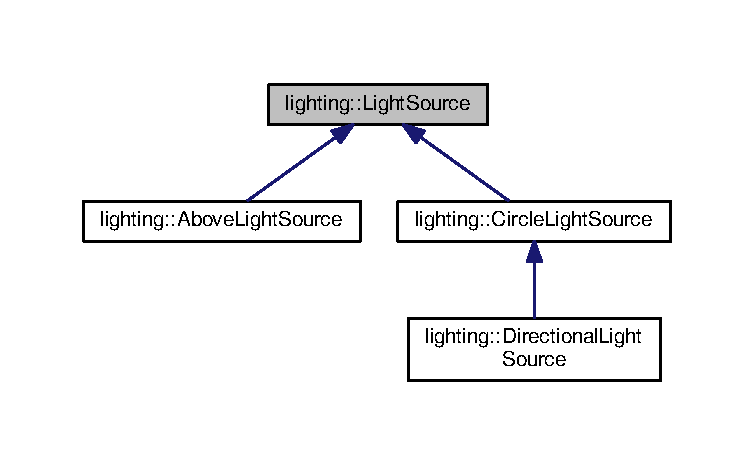
\includegraphics[width=350pt]{classlighting_1_1LightSource__inherit__graph}
\end{center}
\end{figure}


Collaboration diagram for lighting\+:\+:Light\+Source\+:\nopagebreak
\begin{figure}[H]
\begin{center}
\leavevmode
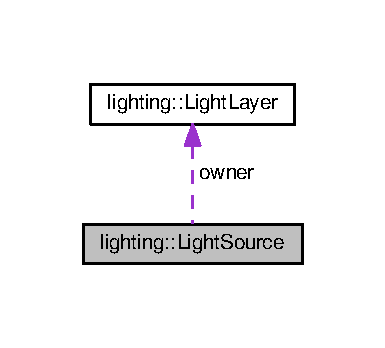
\includegraphics[width=185pt]{classlighting_1_1LightSource__coll__graph}
\end{center}
\end{figure}
\subsection*{Public Member Functions}
\begin{DoxyCompactItemize}
\item 
\hyperlink{classlighting_1_1LightSource_ae03c368df275c4a738c0e0490d9a1e18}{Light\+Source} (\hyperlink{classlighting_1_1LightLayer}{Light\+Layer} $\ast$owner\+Light\+Layer)
\begin{DoxyCompactList}\small\item\em Initializes a new instance of the \hyperlink{classlighting_1_1LightSource}{Light\+Source} class. Will automatically add to the {\itshape owner\+Light\+Layer} . \end{DoxyCompactList}\item 
virtual \hyperlink{classlighting_1_1LightSource_a2165b5cf6099c6e5d2d6d242c1c8113e}{$\sim$\+Light\+Source} ()
\begin{DoxyCompactList}\small\item\em Finalizes an instance of the \hyperlink{classlighting_1_1LightSource}{Light\+Source} class. Removes the {\ttfamily this} from the \hyperlink{classlighting_1_1LightSource_ab991aac9d9ab3a1583f4acdc209055d5}{owner}. \end{DoxyCompactList}\end{DoxyCompactItemize}
\subsection*{Static Public Member Functions}
\begin{DoxyCompactItemize}
\item 
static void \hyperlink{classlighting_1_1LightSource_a1093a521b41e902cbafb92b972617e07}{Init\+L\+Source\+Map} (const std\+::string \&light\+Dir=\hyperlink{classlighting_1_1LightSource_a4455fb30412417b0866c5a953cb55314}{L\+S\+O\+U\+R\+C\+E\+\_\+\+I\+M\+G\+\_\+\+D\+E\+F\+A\+U\+L\+T\+\_\+\+D\+IR})
\begin{DoxyCompactList}\small\item\em Initializes the L\+Source\+Map and all non constant attributes relating to it. \end{DoxyCompactList}\end{DoxyCompactItemize}
\subsection*{Protected Member Functions}
\begin{DoxyCompactItemize}
\item 
virtual void \hyperlink{classlighting_1_1LightSource_a5bf73ee0586ba7620b917e57148d67be}{create\+Shade\+Points} ()=0
\begin{DoxyCompactList}\small\item\em Converts elements of light\+Blockers to \hyperlink{classlighting_1_1ShadePoint}{Shade\+Point}s, populating the vector of \hyperlink{classlighting_1_1ShadePoint}{Shade\+Point}s. \end{DoxyCompactList}\item 
virtual void \hyperlink{classlighting_1_1LightSource_a5bbde61a54af327d43dc4afee751412c}{map\+Shade\+Points} ()=0
\begin{DoxyCompactList}\small\item\em Uses vector of \hyperlink{classlighting_1_1ShadePoint}{Shade\+Point}s to calculate the drawing coordinates. This will handle shadows. \end{DoxyCompactList}\item 
virtual void \hyperlink{classlighting_1_1LightSource_ab15af06660d5cd4658d61ac2075aedea}{draw\+Local} ()=0
\begin{DoxyCompactList}\small\item\em Now that drawing operations are possible, shadows can be drawn to the bitmap data member, if it exists. \end{DoxyCompactList}\item 
virtual void \hyperlink{classlighting_1_1LightSource_a4e292cccdfb5784e97a1924ca00533b9}{draw\+To\+Light\+Map} ()=0
\begin{DoxyCompactList}\small\item\em Draws to the \hyperlink{}{. Assumes light\+Map is already set as the target bitmap. } \end{DoxyCompactList}\item 
virtual void \hyperlink{classlighting_1_1LightSource_ae4be8445f78d1314e112aed9c25933fc}{transfer\+Held\+Vars} ()=0
\begin{DoxyCompactList}\small\item\em When the \hyperlink{classlighting_1_1LightSource}{Light\+Source} is being processed, setting some variables may not be thread safe, so they are stored in held\+Variables, this function tranfers their values. \end{DoxyCompactList}\end{DoxyCompactItemize}
\subsection*{Protected Attributes}
\begin{DoxyCompactItemize}
\item 
\hyperlink{classlighting_1_1LightLayer}{Light\+Layer} $\ast$ \hyperlink{classlighting_1_1LightSource_ab991aac9d9ab3a1583f4acdc209055d5}{owner}
\begin{DoxyCompactList}\small\item\em The owner of 
\begin{DoxyCode}
\textcolor{keyword}{this}
\end{DoxyCode}
. Set by constructor and is not reassigned afterwards. Pointer is used to access light\+BmpW and light\+BmpH for drawing operations. Also allows {\ttfamily this} to remove itself when \hyperlink{classlighting_1_1LightSource_a2165b5cf6099c6e5d2d6d242c1c8113e}{$\sim$\+Light\+Source()} is called. \end{DoxyCompactList}\end{DoxyCompactItemize}
\subsection*{Static Protected Attributes}
\begin{DoxyCompactItemize}
\item 
static const int \hyperlink{classlighting_1_1LightSource_a596474efbeedef2777aeb01e33d845f5}{L\+S\+O\+U\+R\+C\+E\+\_\+\+M\+A\+P\+\_\+\+F\+L\+A\+GS} = A\+L\+L\+E\+G\+R\+O\+\_\+\+M\+I\+N\+\_\+\+L\+I\+N\+E\+AR
\begin{DoxyCompactList}\small\item\em The allegro bitmap flags for loading \hyperlink{classlighting_1_1LightSource_a11a9e08c80631c3019c2a59947c8458e}{L\+Source\+\_\+\+Map} \end{DoxyCompactList}\item 
static const std\+::string \hyperlink{classlighting_1_1LightSource_a4455fb30412417b0866c5a953cb55314}{L\+S\+O\+U\+R\+C\+E\+\_\+\+I\+M\+G\+\_\+\+D\+E\+F\+A\+U\+L\+T\+\_\+\+D\+IR} = \char`\"{}light.\+png\char`\"{}
\begin{DoxyCompactList}\small\item\em The directory to load the \hyperlink{classlighting_1_1LightSource_a11a9e08c80631c3019c2a59947c8458e}{L\+Source\+\_\+\+Map} from. \end{DoxyCompactList}\item 
static A\+L\+L\+E\+G\+R\+O\+\_\+\+B\+I\+T\+M\+AP $\ast$ \hyperlink{classlighting_1_1LightSource_a11a9e08c80631c3019c2a59947c8458e}{L\+Source\+\_\+\+Map} = nullptr
\begin{DoxyCompactList}\small\item\em The bitmap of a circular light, shadows are drawn onto this bitmap. \end{DoxyCompactList}\item 
static int \hyperlink{classlighting_1_1LightSource_a0f364dedbf71ae79f11d1b05fe2863dd}{L\+Source\+\_\+\+Map\+\_\+W} = 0
\begin{DoxyCompactList}\small\item\em The width of \hyperlink{classlighting_1_1LightSource_a11a9e08c80631c3019c2a59947c8458e}{L\+Source\+\_\+\+Map} \end{DoxyCompactList}\item 
static int \hyperlink{classlighting_1_1LightSource_aff96d0ce927829938fe4ed0b07d95448}{L\+Source\+\_\+\+Map\+\_\+H} = 0
\begin{DoxyCompactList}\small\item\em The height of \hyperlink{classlighting_1_1LightSource_a11a9e08c80631c3019c2a59947c8458e}{L\+Source\+\_\+\+Map} \end{DoxyCompactList}\end{DoxyCompactItemize}
\subsection*{Friends}
\begin{DoxyCompactItemize}
\item 
class {\bfseries Light\+Runnable}\hypertarget{classlighting_1_1LightSource_a954406376380fcd34e42954895a037d0}{}\label{classlighting_1_1LightSource_a954406376380fcd34e42954895a037d0}

\item 
class {\bfseries Light\+Layer}\hypertarget{classlighting_1_1LightSource_aa4da5897890a726ecc5247c37419663b}{}\label{classlighting_1_1LightSource_aa4da5897890a726ecc5247c37419663b}

\end{DoxyCompactItemize}


\subsection{Detailed Description}
Abstract class represnting an light that can be blocked 



\subsection{Constructor \& Destructor Documentation}
\index{lighting\+::\+Light\+Source@{lighting\+::\+Light\+Source}!Light\+Source@{Light\+Source}}
\index{Light\+Source@{Light\+Source}!lighting\+::\+Light\+Source@{lighting\+::\+Light\+Source}}
\subsubsection[{\texorpdfstring{Light\+Source(\+Light\+Layer $\ast$owner\+Light\+Layer)}{LightSource(LightLayer *ownerLightLayer)}}]{\setlength{\rightskip}{0pt plus 5cm}lighting\+::\+Light\+Source\+::\+Light\+Source (
\begin{DoxyParamCaption}
\item[{{\bf Light\+Layer} $\ast$}]{owner\+Light\+Layer}
\end{DoxyParamCaption}
)}\hypertarget{classlighting_1_1LightSource_ae03c368df275c4a738c0e0490d9a1e18}{}\label{classlighting_1_1LightSource_ae03c368df275c4a738c0e0490d9a1e18}


Initializes a new instance of the \hyperlink{classlighting_1_1LightSource}{Light\+Source} class. Will automatically add to the {\itshape owner\+Light\+Layer} . 


\begin{DoxyParams}{Parameters}
{\em owner\+Light\+Layer} & The light layer that will own {\ttfamily this}. Value is assigned to \hyperlink{classlighting_1_1LightSource_ab991aac9d9ab3a1583f4acdc209055d5}{owner}\\
\hline
\end{DoxyParams}
\index{lighting\+::\+Light\+Source@{lighting\+::\+Light\+Source}!````~Light\+Source@{$\sim$\+Light\+Source}}
\index{````~Light\+Source@{$\sim$\+Light\+Source}!lighting\+::\+Light\+Source@{lighting\+::\+Light\+Source}}
\subsubsection[{\texorpdfstring{$\sim$\+Light\+Source()}{~LightSource()}}]{\setlength{\rightskip}{0pt plus 5cm}lighting\+::\+Light\+Source\+::$\sim$\+Light\+Source (
\begin{DoxyParamCaption}
{}
\end{DoxyParamCaption}
)\hspace{0.3cm}{\ttfamily [virtual]}}\hypertarget{classlighting_1_1LightSource_a2165b5cf6099c6e5d2d6d242c1c8113e}{}\label{classlighting_1_1LightSource_a2165b5cf6099c6e5d2d6d242c1c8113e}


Finalizes an instance of the \hyperlink{classlighting_1_1LightSource}{Light\+Source} class. Removes the {\ttfamily this} from the \hyperlink{classlighting_1_1LightSource_ab991aac9d9ab3a1583f4acdc209055d5}{owner}. 



\subsection{Member Function Documentation}
\index{lighting\+::\+Light\+Source@{lighting\+::\+Light\+Source}!create\+Shade\+Points@{create\+Shade\+Points}}
\index{create\+Shade\+Points@{create\+Shade\+Points}!lighting\+::\+Light\+Source@{lighting\+::\+Light\+Source}}
\subsubsection[{\texorpdfstring{create\+Shade\+Points()=0}{createShadePoints()=0}}]{\setlength{\rightskip}{0pt plus 5cm}virtual void lighting\+::\+Light\+Source\+::create\+Shade\+Points (
\begin{DoxyParamCaption}
{}
\end{DoxyParamCaption}
)\hspace{0.3cm}{\ttfamily [protected]}, {\ttfamily [pure virtual]}}\hypertarget{classlighting_1_1LightSource_a5bf73ee0586ba7620b917e57148d67be}{}\label{classlighting_1_1LightSource_a5bf73ee0586ba7620b917e57148d67be}


Converts elements of light\+Blockers to \hyperlink{classlighting_1_1ShadePoint}{Shade\+Point}s, populating the vector of \hyperlink{classlighting_1_1ShadePoint}{Shade\+Point}s. 



Implemented in \hyperlink{classlighting_1_1CircleLightSource_aaa80bb9a9a27f3c74bf86cfd547d5f36}{lighting\+::\+Circle\+Light\+Source}, and \hyperlink{classlighting_1_1AboveLightSource_a13665ac64b61239624b430a49ab609ab}{lighting\+::\+Above\+Light\+Source}.

\index{lighting\+::\+Light\+Source@{lighting\+::\+Light\+Source}!draw\+Local@{draw\+Local}}
\index{draw\+Local@{draw\+Local}!lighting\+::\+Light\+Source@{lighting\+::\+Light\+Source}}
\subsubsection[{\texorpdfstring{draw\+Local()=0}{drawLocal()=0}}]{\setlength{\rightskip}{0pt plus 5cm}virtual void lighting\+::\+Light\+Source\+::draw\+Local (
\begin{DoxyParamCaption}
{}
\end{DoxyParamCaption}
)\hspace{0.3cm}{\ttfamily [protected]}, {\ttfamily [pure virtual]}}\hypertarget{classlighting_1_1LightSource_ab15af06660d5cd4658d61ac2075aedea}{}\label{classlighting_1_1LightSource_ab15af06660d5cd4658d61ac2075aedea}


Now that drawing operations are possible, shadows can be drawn to the bitmap data member, if it exists. 



Implemented in \hyperlink{classlighting_1_1CircleLightSource_a6ab6f8f8eaf003e52ac2c86d88496c77}{lighting\+::\+Circle\+Light\+Source}, \hyperlink{classlighting_1_1AboveLightSource_af858515032138900888d8db1a5f6812d}{lighting\+::\+Above\+Light\+Source}, and \hyperlink{classlighting_1_1DirectionalLightSource_a52f9f09a4088a44bf3f8b08df435a7aa}{lighting\+::\+Directional\+Light\+Source}.

\index{lighting\+::\+Light\+Source@{lighting\+::\+Light\+Source}!draw\+To\+Light\+Map@{draw\+To\+Light\+Map}}
\index{draw\+To\+Light\+Map@{draw\+To\+Light\+Map}!lighting\+::\+Light\+Source@{lighting\+::\+Light\+Source}}
\subsubsection[{\texorpdfstring{draw\+To\+Light\+Map()=0}{drawToLightMap()=0}}]{\setlength{\rightskip}{0pt plus 5cm}virtual void lighting\+::\+Light\+Source\+::draw\+To\+Light\+Map (
\begin{DoxyParamCaption}
{}
\end{DoxyParamCaption}
)\hspace{0.3cm}{\ttfamily [protected]}, {\ttfamily [pure virtual]}}\hypertarget{classlighting_1_1LightSource_a4e292cccdfb5784e97a1924ca00533b9}{}\label{classlighting_1_1LightSource_a4e292cccdfb5784e97a1924ca00533b9}


Draws to the \hyperlink{}{. Assumes light\+Map is already set as the target bitmap. } 



Implemented in \hyperlink{classlighting_1_1CircleLightSource_ab0f9107c09ae9c6966bab14538505894}{lighting\+::\+Circle\+Light\+Source}, \hyperlink{classlighting_1_1AboveLightSource_ae941abaa5da73f24c11d1e2c120af9ae}{lighting\+::\+Above\+Light\+Source}, and \hyperlink{classlighting_1_1DirectionalLightSource_ab41be6321df178f861cd71462ab47553}{lighting\+::\+Directional\+Light\+Source}.

\index{lighting\+::\+Light\+Source@{lighting\+::\+Light\+Source}!Init\+L\+Source\+Map@{Init\+L\+Source\+Map}}
\index{Init\+L\+Source\+Map@{Init\+L\+Source\+Map}!lighting\+::\+Light\+Source@{lighting\+::\+Light\+Source}}
\subsubsection[{\texorpdfstring{Init\+L\+Source\+Map(const std\+::string \&light\+Dir=\+L\+S\+O\+U\+R\+C\+E\+\_\+\+I\+M\+G\+\_\+\+D\+E\+F\+A\+U\+L\+T\+\_\+\+D\+I\+R)}{InitLSourceMap(const std::string &lightDir=LSOURCE_IMG_DEFAULT_DIR)}}]{\setlength{\rightskip}{0pt plus 5cm}void lighting\+::\+Light\+Source\+::\+Init\+L\+Source\+Map (
\begin{DoxyParamCaption}
\item[{const std\+::string \&}]{light\+Dir = {\ttfamily {\bf L\+S\+O\+U\+R\+C\+E\+\_\+\+I\+M\+G\+\_\+\+D\+E\+F\+A\+U\+L\+T\+\_\+\+D\+IR}}}
\end{DoxyParamCaption}
)\hspace{0.3cm}{\ttfamily [static]}}\hypertarget{classlighting_1_1LightSource_a1093a521b41e902cbafb92b972617e07}{}\label{classlighting_1_1LightSource_a1093a521b41e902cbafb92b972617e07}


Initializes the L\+Source\+Map and all non constant attributes relating to it. 


\begin{DoxyParams}{Parameters}
{\em path} & File to load bitmap from. Set to \hyperlink{classlighting_1_1LightSource_a4455fb30412417b0866c5a953cb55314}{L\+S\+O\+U\+R\+C\+E\+\_\+\+I\+M\+G\+\_\+\+D\+E\+F\+A\+U\+L\+T\+\_\+\+D\+IR} by default.\\
\hline
\end{DoxyParams}
\index{lighting\+::\+Light\+Source@{lighting\+::\+Light\+Source}!map\+Shade\+Points@{map\+Shade\+Points}}
\index{map\+Shade\+Points@{map\+Shade\+Points}!lighting\+::\+Light\+Source@{lighting\+::\+Light\+Source}}
\subsubsection[{\texorpdfstring{map\+Shade\+Points()=0}{mapShadePoints()=0}}]{\setlength{\rightskip}{0pt plus 5cm}virtual void lighting\+::\+Light\+Source\+::map\+Shade\+Points (
\begin{DoxyParamCaption}
{}
\end{DoxyParamCaption}
)\hspace{0.3cm}{\ttfamily [protected]}, {\ttfamily [pure virtual]}}\hypertarget{classlighting_1_1LightSource_a5bbde61a54af327d43dc4afee751412c}{}\label{classlighting_1_1LightSource_a5bbde61a54af327d43dc4afee751412c}


Uses vector of \hyperlink{classlighting_1_1ShadePoint}{Shade\+Point}s to calculate the drawing coordinates. This will handle shadows. 



Implemented in \hyperlink{classlighting_1_1CircleLightSource_aea43f0005a2ffbc50e8898e2e967693b}{lighting\+::\+Circle\+Light\+Source}, and \hyperlink{classlighting_1_1AboveLightSource_a9331dd2674565685388ef044b71a4881}{lighting\+::\+Above\+Light\+Source}.

\index{lighting\+::\+Light\+Source@{lighting\+::\+Light\+Source}!transfer\+Held\+Vars@{transfer\+Held\+Vars}}
\index{transfer\+Held\+Vars@{transfer\+Held\+Vars}!lighting\+::\+Light\+Source@{lighting\+::\+Light\+Source}}
\subsubsection[{\texorpdfstring{transfer\+Held\+Vars()=0}{transferHeldVars()=0}}]{\setlength{\rightskip}{0pt plus 5cm}virtual void lighting\+::\+Light\+Source\+::transfer\+Held\+Vars (
\begin{DoxyParamCaption}
{}
\end{DoxyParamCaption}
)\hspace{0.3cm}{\ttfamily [protected]}, {\ttfamily [pure virtual]}}\hypertarget{classlighting_1_1LightSource_ae4be8445f78d1314e112aed9c25933fc}{}\label{classlighting_1_1LightSource_ae4be8445f78d1314e112aed9c25933fc}


When the \hyperlink{classlighting_1_1LightSource}{Light\+Source} is being processed, setting some variables may not be thread safe, so they are stored in held\+Variables, this function tranfers their values. 



Implemented in \hyperlink{classlighting_1_1CircleLightSource_afc39570a33c19b17fb8153be592b01e9}{lighting\+::\+Circle\+Light\+Source}, and \hyperlink{classlighting_1_1AboveLightSource_a4b18ea492b7f63bc34f7bd269317c20e}{lighting\+::\+Above\+Light\+Source}.



\subsection{Member Data Documentation}
\index{lighting\+::\+Light\+Source@{lighting\+::\+Light\+Source}!L\+S\+O\+U\+R\+C\+E\+\_\+\+I\+M\+G\+\_\+\+D\+E\+F\+A\+U\+L\+T\+\_\+\+D\+IR@{L\+S\+O\+U\+R\+C\+E\+\_\+\+I\+M\+G\+\_\+\+D\+E\+F\+A\+U\+L\+T\+\_\+\+D\+IR}}
\index{L\+S\+O\+U\+R\+C\+E\+\_\+\+I\+M\+G\+\_\+\+D\+E\+F\+A\+U\+L\+T\+\_\+\+D\+IR@{L\+S\+O\+U\+R\+C\+E\+\_\+\+I\+M\+G\+\_\+\+D\+E\+F\+A\+U\+L\+T\+\_\+\+D\+IR}!lighting\+::\+Light\+Source@{lighting\+::\+Light\+Source}}
\subsubsection[{\texorpdfstring{L\+S\+O\+U\+R\+C\+E\+\_\+\+I\+M\+G\+\_\+\+D\+E\+F\+A\+U\+L\+T\+\_\+\+D\+IR}{LSOURCE_IMG_DEFAULT_DIR}}]{\setlength{\rightskip}{0pt plus 5cm}const std\+::string lighting\+::\+Light\+Source\+::\+L\+S\+O\+U\+R\+C\+E\+\_\+\+I\+M\+G\+\_\+\+D\+E\+F\+A\+U\+L\+T\+\_\+\+D\+IR = \char`\"{}light.\+png\char`\"{}\hspace{0.3cm}{\ttfamily [static]}, {\ttfamily [protected]}}\hypertarget{classlighting_1_1LightSource_a4455fb30412417b0866c5a953cb55314}{}\label{classlighting_1_1LightSource_a4455fb30412417b0866c5a953cb55314}


The directory to load the \hyperlink{classlighting_1_1LightSource_a11a9e08c80631c3019c2a59947c8458e}{L\+Source\+\_\+\+Map} from. 

\index{lighting\+::\+Light\+Source@{lighting\+::\+Light\+Source}!L\+Source\+\_\+\+Map@{L\+Source\+\_\+\+Map}}
\index{L\+Source\+\_\+\+Map@{L\+Source\+\_\+\+Map}!lighting\+::\+Light\+Source@{lighting\+::\+Light\+Source}}
\subsubsection[{\texorpdfstring{L\+Source\+\_\+\+Map}{LSource_Map}}]{\setlength{\rightskip}{0pt plus 5cm}A\+L\+L\+E\+G\+R\+O\+\_\+\+B\+I\+T\+M\+AP $\ast$ lighting\+::\+Light\+Source\+::\+L\+Source\+\_\+\+Map = nullptr\hspace{0.3cm}{\ttfamily [static]}, {\ttfamily [protected]}}\hypertarget{classlighting_1_1LightSource_a11a9e08c80631c3019c2a59947c8458e}{}\label{classlighting_1_1LightSource_a11a9e08c80631c3019c2a59947c8458e}


The bitmap of a circular light, shadows are drawn onto this bitmap. 

\index{lighting\+::\+Light\+Source@{lighting\+::\+Light\+Source}!L\+S\+O\+U\+R\+C\+E\+\_\+\+M\+A\+P\+\_\+\+F\+L\+A\+GS@{L\+S\+O\+U\+R\+C\+E\+\_\+\+M\+A\+P\+\_\+\+F\+L\+A\+GS}}
\index{L\+S\+O\+U\+R\+C\+E\+\_\+\+M\+A\+P\+\_\+\+F\+L\+A\+GS@{L\+S\+O\+U\+R\+C\+E\+\_\+\+M\+A\+P\+\_\+\+F\+L\+A\+GS}!lighting\+::\+Light\+Source@{lighting\+::\+Light\+Source}}
\subsubsection[{\texorpdfstring{L\+S\+O\+U\+R\+C\+E\+\_\+\+M\+A\+P\+\_\+\+F\+L\+A\+GS}{LSOURCE_MAP_FLAGS}}]{\setlength{\rightskip}{0pt plus 5cm}const int lighting\+::\+Light\+Source\+::\+L\+S\+O\+U\+R\+C\+E\+\_\+\+M\+A\+P\+\_\+\+F\+L\+A\+GS = A\+L\+L\+E\+G\+R\+O\+\_\+\+M\+I\+N\+\_\+\+L\+I\+N\+E\+AR\hspace{0.3cm}{\ttfamily [static]}, {\ttfamily [protected]}}\hypertarget{classlighting_1_1LightSource_a596474efbeedef2777aeb01e33d845f5}{}\label{classlighting_1_1LightSource_a596474efbeedef2777aeb01e33d845f5}


The allegro bitmap flags for loading \hyperlink{classlighting_1_1LightSource_a11a9e08c80631c3019c2a59947c8458e}{L\+Source\+\_\+\+Map} 

\index{lighting\+::\+Light\+Source@{lighting\+::\+Light\+Source}!L\+Source\+\_\+\+Map\+\_\+H@{L\+Source\+\_\+\+Map\+\_\+H}}
\index{L\+Source\+\_\+\+Map\+\_\+H@{L\+Source\+\_\+\+Map\+\_\+H}!lighting\+::\+Light\+Source@{lighting\+::\+Light\+Source}}
\subsubsection[{\texorpdfstring{L\+Source\+\_\+\+Map\+\_\+H}{LSource_Map_H}}]{\setlength{\rightskip}{0pt plus 5cm}int lighting\+::\+Light\+Source\+::\+L\+Source\+\_\+\+Map\+\_\+H = 0\hspace{0.3cm}{\ttfamily [static]}, {\ttfamily [protected]}}\hypertarget{classlighting_1_1LightSource_aff96d0ce927829938fe4ed0b07d95448}{}\label{classlighting_1_1LightSource_aff96d0ce927829938fe4ed0b07d95448}


The height of \hyperlink{classlighting_1_1LightSource_a11a9e08c80631c3019c2a59947c8458e}{L\+Source\+\_\+\+Map} 

\index{lighting\+::\+Light\+Source@{lighting\+::\+Light\+Source}!L\+Source\+\_\+\+Map\+\_\+W@{L\+Source\+\_\+\+Map\+\_\+W}}
\index{L\+Source\+\_\+\+Map\+\_\+W@{L\+Source\+\_\+\+Map\+\_\+W}!lighting\+::\+Light\+Source@{lighting\+::\+Light\+Source}}
\subsubsection[{\texorpdfstring{L\+Source\+\_\+\+Map\+\_\+W}{LSource_Map_W}}]{\setlength{\rightskip}{0pt plus 5cm}int lighting\+::\+Light\+Source\+::\+L\+Source\+\_\+\+Map\+\_\+W = 0\hspace{0.3cm}{\ttfamily [static]}, {\ttfamily [protected]}}\hypertarget{classlighting_1_1LightSource_a0f364dedbf71ae79f11d1b05fe2863dd}{}\label{classlighting_1_1LightSource_a0f364dedbf71ae79f11d1b05fe2863dd}


The width of \hyperlink{classlighting_1_1LightSource_a11a9e08c80631c3019c2a59947c8458e}{L\+Source\+\_\+\+Map} 

\index{lighting\+::\+Light\+Source@{lighting\+::\+Light\+Source}!owner@{owner}}
\index{owner@{owner}!lighting\+::\+Light\+Source@{lighting\+::\+Light\+Source}}
\subsubsection[{\texorpdfstring{owner}{owner}}]{\setlength{\rightskip}{0pt plus 5cm}{\bf Light\+Layer}$\ast$ lighting\+::\+Light\+Source\+::owner\hspace{0.3cm}{\ttfamily [protected]}}\hypertarget{classlighting_1_1LightSource_ab991aac9d9ab3a1583f4acdc209055d5}{}\label{classlighting_1_1LightSource_ab991aac9d9ab3a1583f4acdc209055d5}


The owner of 
\begin{DoxyCode}
\textcolor{keyword}{this}
\end{DoxyCode}
. Set by constructor and is not reassigned afterwards. Pointer is used to access light\+BmpW and light\+BmpH for drawing operations. Also allows {\ttfamily this} to remove itself when \hyperlink{classlighting_1_1LightSource_a2165b5cf6099c6e5d2d6d242c1c8113e}{$\sim$\+Light\+Source()} is called. 



The documentation for this class was generated from the following files\+:\begin{DoxyCompactItemize}
\item 
Light\+Source.\+h\item 
Light\+Source.\+cpp\end{DoxyCompactItemize}

\hypertarget{classlighting_1_1ShadePoint}{}\section{lighting\+:\+:Shade\+Point Class Reference}
\label{classlighting_1_1ShadePoint}\index{lighting\+::\+Shade\+Point@{lighting\+::\+Shade\+Point}}


Inheritance diagram for lighting\+:\+:Shade\+Point\+:\nopagebreak
\begin{figure}[H]
\begin{center}
\leavevmode
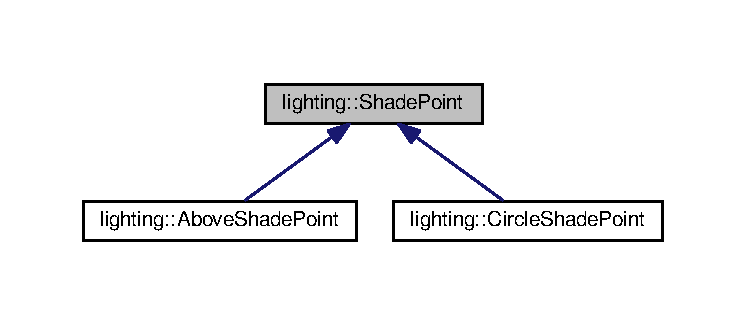
\includegraphics[width=350pt]{classlighting_1_1ShadePoint__inherit__graph}
\end{center}
\end{figure}


Collaboration diagram for lighting\+:\+:Shade\+Point\+:\nopagebreak
\begin{figure}[H]
\begin{center}
\leavevmode
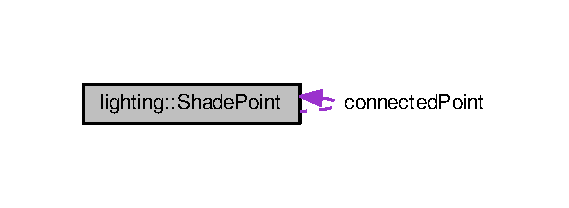
\includegraphics[width=273pt]{classlighting_1_1ShadePoint__coll__graph}
\end{center}
\end{figure}
\subsection*{Public Member Functions}
\begin{DoxyCompactItemize}
\item 
\hyperlink{classlighting_1_1ShadePoint_aaebbffa8b934868a07455343a1943e25}{Shade\+Point} (float \hyperlink{classlighting_1_1ShadePoint_a087db3eacccf6731f674f123c22400ec}{x}, float \hyperlink{classlighting_1_1ShadePoint_a427350496a448f0dd7424955a6c21ea2}{y})
\begin{DoxyCompactList}\small\item\em Assigns the local coordinates to the parameters and calculates the angle of those values from the origin (0, 0). \end{DoxyCompactList}\item 
void \hyperlink{classlighting_1_1ShadePoint_a6d8d66a55dd8b16974bf138bbfcac183}{set\+Connect\+Point} (\hyperlink{classlighting_1_1ShadePoint}{Shade\+Point} $\ast$connect\+Point)
\begin{DoxyCompactList}\small\item\em Modifier for the attribute \hyperlink{classlighting_1_1ShadePoint_a0840495febcd385a90e89e003aa15972}{Shade\+Point\+::connected\+Point}. Represents the other endpoint of a line. \end{DoxyCompactList}\item 
bool \hyperlink{classlighting_1_1ShadePoint_af520192e696fc33d0aec19f0f4519a28}{check\+Intersect} (float x1, float y1, float x2, float y2, float \&cX, float \&cY)
\begin{DoxyCompactList}\small\item\em Checks if the endpoints passed in as parameters form a line that would intersect with a line formed by connecting the coordinates from {\ttfamily  this } \hyperlink{classlighting_1_1ShadePoint}{Shade\+Point}s coordinates to the coordinates from \hyperlink{classlighting_1_1ShadePoint_a0840495febcd385a90e89e003aa15972}{Shade\+Point\+::connected\+Point}. \end{DoxyCompactList}\item 
virtual \hyperlink{classlighting_1_1ShadePoint_a87875dcdefcbf587d2a060831b2ec628}{$\sim$\+Shade\+Point} ()
\begin{DoxyCompactList}\small\item\em Finalizes an instance of the \hyperlink{classlighting_1_1ShadePoint}{Shade\+Point} class. Note that \hyperlink{classlighting_1_1ShadePoint_a0840495febcd385a90e89e003aa15972}{Shade\+Point\+::connected\+Point} will not be deleted. \end{DoxyCompactList}\end{DoxyCompactItemize}
\subsection*{Public Attributes}
\begin{DoxyCompactItemize}
\item 
float \hyperlink{classlighting_1_1ShadePoint_a087db3eacccf6731f674f123c22400ec}{x}
\begin{DoxyCompactList}\small\item\em The horizontal position of the point. \end{DoxyCompactList}\item 
float \hyperlink{classlighting_1_1ShadePoint_a427350496a448f0dd7424955a6c21ea2}{y}
\begin{DoxyCompactList}\small\item\em The horizontal position of the point. \end{DoxyCompactList}\end{DoxyCompactItemize}
\subsection*{Protected Attributes}
\begin{DoxyCompactItemize}
\item 
\hyperlink{classlighting_1_1ShadePoint}{Shade\+Point} $\ast$ \hyperlink{classlighting_1_1ShadePoint_a0840495febcd385a90e89e003aa15972}{connected\+Point}
\begin{DoxyCompactList}\small\item\em The other endpoint of the line. Initially set to {\ttfamily nullptr} but can be set by the method \hyperlink{classlighting_1_1ShadePoint_a6d8d66a55dd8b16974bf138bbfcac183}{Shade\+Point\+::set\+Connect\+Point(\+Shade\+Point$\ast$)}. \end{DoxyCompactList}\end{DoxyCompactItemize}


\subsection{Constructor \& Destructor Documentation}
\index{lighting\+::\+Shade\+Point@{lighting\+::\+Shade\+Point}!Shade\+Point@{Shade\+Point}}
\index{Shade\+Point@{Shade\+Point}!lighting\+::\+Shade\+Point@{lighting\+::\+Shade\+Point}}
\subsubsection[{\texorpdfstring{Shade\+Point(float x, float y)}{ShadePoint(float x, float y)}}]{\setlength{\rightskip}{0pt plus 5cm}lighting\+::\+Shade\+Point\+::\+Shade\+Point (
\begin{DoxyParamCaption}
\item[{float}]{x, }
\item[{float}]{y}
\end{DoxyParamCaption}
)}\hypertarget{classlighting_1_1ShadePoint_aaebbffa8b934868a07455343a1943e25}{}\label{classlighting_1_1ShadePoint_aaebbffa8b934868a07455343a1943e25}


Assigns the local coordinates to the parameters and calculates the angle of those values from the origin (0, 0). 


\begin{DoxyParams}{Parameters}
{\em x} & The horizontal coordinate of the point.\\
\hline
{\em y} & The vertical coordinate of the point.\\
\hline
\end{DoxyParams}
\index{lighting\+::\+Shade\+Point@{lighting\+::\+Shade\+Point}!````~Shade\+Point@{$\sim$\+Shade\+Point}}
\index{````~Shade\+Point@{$\sim$\+Shade\+Point}!lighting\+::\+Shade\+Point@{lighting\+::\+Shade\+Point}}
\subsubsection[{\texorpdfstring{$\sim$\+Shade\+Point()}{~ShadePoint()}}]{\setlength{\rightskip}{0pt plus 5cm}lighting\+::\+Shade\+Point\+::$\sim$\+Shade\+Point (
\begin{DoxyParamCaption}
{}
\end{DoxyParamCaption}
)\hspace{0.3cm}{\ttfamily [virtual]}}\hypertarget{classlighting_1_1ShadePoint_a87875dcdefcbf587d2a060831b2ec628}{}\label{classlighting_1_1ShadePoint_a87875dcdefcbf587d2a060831b2ec628}


Finalizes an instance of the \hyperlink{classlighting_1_1ShadePoint}{Shade\+Point} class. Note that \hyperlink{classlighting_1_1ShadePoint_a0840495febcd385a90e89e003aa15972}{Shade\+Point\+::connected\+Point} will not be deleted. 



\subsection{Member Function Documentation}
\index{lighting\+::\+Shade\+Point@{lighting\+::\+Shade\+Point}!check\+Intersect@{check\+Intersect}}
\index{check\+Intersect@{check\+Intersect}!lighting\+::\+Shade\+Point@{lighting\+::\+Shade\+Point}}
\subsubsection[{\texorpdfstring{check\+Intersect(float x1, float y1, float x2, float y2, float \&c\+X, float \&c\+Y)}{checkIntersect(float x1, float y1, float x2, float y2, float &cX, float &cY)}}]{\setlength{\rightskip}{0pt plus 5cm}bool lighting\+::\+Shade\+Point\+::check\+Intersect (
\begin{DoxyParamCaption}
\item[{float}]{x1, }
\item[{float}]{y1, }
\item[{float}]{x2, }
\item[{float}]{y2, }
\item[{float \&}]{cX, }
\item[{float \&}]{cY}
\end{DoxyParamCaption}
)}\hypertarget{classlighting_1_1ShadePoint_af520192e696fc33d0aec19f0f4519a28}{}\label{classlighting_1_1ShadePoint_af520192e696fc33d0aec19f0f4519a28}


Checks if the endpoints passed in as parameters form a line that would intersect with a line formed by connecting the coordinates from {\ttfamily  this } \hyperlink{classlighting_1_1ShadePoint}{Shade\+Point}s coordinates to the coordinates from \hyperlink{classlighting_1_1ShadePoint_a0840495febcd385a90e89e003aa15972}{Shade\+Point\+::connected\+Point}. 


\begin{DoxyParams}{Parameters}
{\em x1} & The horizontal position of the first endpoint.\\
\hline
{\em y1} & The vertical position of the first endpoint.\\
\hline
{\em x2} & The horizontal position of the second endpoint.\\
\hline
{\em y2} & The vertical position of the second endpoint.\\
\hline
{\em cX} & Serves as an output parameter. If a collision occurs, the value will represent the horizontal position of the collision. Otherwise, it is unmodified.\\
\hline
{\em cY} & Serves as an output parameter. If a collision occurs, the value will represent the vertical position of the collision. Otherwise, it is unmodified.\\
\hline
\end{DoxyParams}
\begin{DoxyReturn}{Returns}
{\ttfamily true} if the lines intersected. {\ttfamily false} otherwise.
\end{DoxyReturn}
\index{lighting\+::\+Shade\+Point@{lighting\+::\+Shade\+Point}!set\+Connect\+Point@{set\+Connect\+Point}}
\index{set\+Connect\+Point@{set\+Connect\+Point}!lighting\+::\+Shade\+Point@{lighting\+::\+Shade\+Point}}
\subsubsection[{\texorpdfstring{set\+Connect\+Point(\+Shade\+Point $\ast$connect\+Point)}{setConnectPoint(ShadePoint *connectPoint)}}]{\setlength{\rightskip}{0pt plus 5cm}void lighting\+::\+Shade\+Point\+::set\+Connect\+Point (
\begin{DoxyParamCaption}
\item[{{\bf Shade\+Point} $\ast$}]{connect\+Point}
\end{DoxyParamCaption}
)\hspace{0.3cm}{\ttfamily [inline]}}\hypertarget{classlighting_1_1ShadePoint_a6d8d66a55dd8b16974bf138bbfcac183}{}\label{classlighting_1_1ShadePoint_a6d8d66a55dd8b16974bf138bbfcac183}


Modifier for the attribute \hyperlink{classlighting_1_1ShadePoint_a0840495febcd385a90e89e003aa15972}{Shade\+Point\+::connected\+Point}. Represents the other endpoint of a line. 


\begin{DoxyParams}{Parameters}
{\em connect\+Point} & \\
\hline
\end{DoxyParams}


\subsection{Member Data Documentation}
\index{lighting\+::\+Shade\+Point@{lighting\+::\+Shade\+Point}!connected\+Point@{connected\+Point}}
\index{connected\+Point@{connected\+Point}!lighting\+::\+Shade\+Point@{lighting\+::\+Shade\+Point}}
\subsubsection[{\texorpdfstring{connected\+Point}{connectedPoint}}]{\setlength{\rightskip}{0pt plus 5cm}{\bf Shade\+Point}$\ast$ lighting\+::\+Shade\+Point\+::connected\+Point\hspace{0.3cm}{\ttfamily [protected]}}\hypertarget{classlighting_1_1ShadePoint_a0840495febcd385a90e89e003aa15972}{}\label{classlighting_1_1ShadePoint_a0840495febcd385a90e89e003aa15972}


The other endpoint of the line. Initially set to {\ttfamily nullptr} but can be set by the method \hyperlink{classlighting_1_1ShadePoint_a6d8d66a55dd8b16974bf138bbfcac183}{Shade\+Point\+::set\+Connect\+Point(\+Shade\+Point$\ast$)}. 

\index{lighting\+::\+Shade\+Point@{lighting\+::\+Shade\+Point}!x@{x}}
\index{x@{x}!lighting\+::\+Shade\+Point@{lighting\+::\+Shade\+Point}}
\subsubsection[{\texorpdfstring{x}{x}}]{\setlength{\rightskip}{0pt plus 5cm}float lighting\+::\+Shade\+Point\+::x}\hypertarget{classlighting_1_1ShadePoint_a087db3eacccf6731f674f123c22400ec}{}\label{classlighting_1_1ShadePoint_a087db3eacccf6731f674f123c22400ec}


The horizontal position of the point. 

\index{lighting\+::\+Shade\+Point@{lighting\+::\+Shade\+Point}!y@{y}}
\index{y@{y}!lighting\+::\+Shade\+Point@{lighting\+::\+Shade\+Point}}
\subsubsection[{\texorpdfstring{y}{y}}]{\setlength{\rightskip}{0pt plus 5cm}float lighting\+::\+Shade\+Point\+::y}\hypertarget{classlighting_1_1ShadePoint_a427350496a448f0dd7424955a6c21ea2}{}\label{classlighting_1_1ShadePoint_a427350496a448f0dd7424955a6c21ea2}


The horizontal position of the point. 



The documentation for this class was generated from the following files\+:\begin{DoxyCompactItemize}
\item 
Shade\+Point.\+h\item 
Shade\+Point.\+cpp\end{DoxyCompactItemize}

%--- End generated contents ---

% Index
\backmatter
\newpage
\phantomsection
\clearemptydoublepage
\addcontentsline{toc}{chapter}{Index}
\printindex

\end{document}
